% ******************************************************************************
% *
% * MODULE Assignment 1
% *
% * DESCRIPTION
% *
% * This file contains the setup procedure for Raspberry Pi 3
% *
% * AUTHOR
% *
% * Andrew N. Sloss
% *
% *

\documentclass{article} 
\usepackage{blindtext}
\usepackage[utf8]{inputenc}
\usepackage{graphicx}
\usepackage{listings}
\usepackage[section]{placeins}
\usepackage[margin=1.0in]{geometry}
\usepackage{lmodern}
% \renewcommand{\familydefault}{\sfdefault}
\usepackage{float}
\usepackage{makeidx}
\newcommand*{\escape}[1]{\texttt{\textbackslash#1}}

\lstset{language=C}  

\graphicspath{{../pdf/}{images/}}

% \renewcommand{\listfigurename}{Figures}
 
\renewcommand{\listtablename}{Tables}

\setlength\parindent{0pt}

\makeindex

\begin{document}


\title{\textbf{C Language - A Modern Approach to Embedded Programming}}
\author{Andrew N. Sloss}
\date{\today}


\maketitle
\begin{abstract}
\noindent
This book is an introduction to the \textbf{C Programming Language}. It is not meant to be an exhaustive introduction or even a replacement of the available teaching books. It has been written to get motivated people up to speed quickly and become somewhat proficient in C, with an emphasis on embedded systems. Use this text as a springboard to explore more.
\end{abstract}

\newpage

\tableofcontents

\newpage

\lstlistoflistings

\newpage

\thispagestyle{empty}
 
\listoffigures
 
\listoftables
 
\clearpage
 
\pagenumbering{arabic}


% *****
%
% Introduction
%
% *****

\section*{Acknowledgements}

Appreciation goes to the 2016-18 students on the Electrical Engineering Professional Masters Program at the University of Washington. Who helped identify the need for a book getting people quickly up-to-speed on the C Programming Language.\\

Also many thanks goes to Ian Field, James McNiven, John Archibald, Alex Finestead and Adam Glass for the valuable feedback and insights provided throughout the construction of this book. A book is only as good as the reviewers.


\newpage
\section{Introduction}

The C Programming Language first appeared in 1972. It was originally designed and developed by Dennis Ritchie. Since the first release the language has gone through a number of major revisions. Today's C language is much improved from the original but continues to retain many of the fundamental qualities and attributes that made it popular.\\ 

There are a number of modern competitors to the C language, such as \textit{Go} and \textit{Rust}. Despite these alternatives, C continues to have a strong following, especially among embedded and system-software engineers. There is a vast wealth of software available and it remains in the top most popular languages on GitHub. The popularity stems from three core attributes, namely simplicity, efficiency and flexibility.\\

Simplicity, the entire definition of the language fits on a few pages of Backus-Naur Form (BNF). If unfamiliar with BNF it is worth taking some time doing some research. BNF is a grammar used to describe programming languages. It has roots dating back to the release of \textit{Algol 58}.\\

Efficiency, the compilers are both mature and highly sophisticated. C converts extremely efficiently to the underlying hardware architecture. And likewise due to its popularity and importance many of today's hardware architectures have been directly influenced by C. A low-level compiled C program is significantly faster than high-level interpreted or abstracted languages such as \textit{Python} or \textit{JavaScript}.\\

Flexibility, the C language provides little in the way of runtime protection against errors. Compilers have improved in recent years but still allow dangerous activity. The dangerous side is important when interfacing with exotic hardware. It is this feature which allows C to be extremely powerful. Stability is in the hands of the programmer i.e. with great power comes great responsibility.\\

To emphasize these advantages, a paper released 2017 at the Software Language Engineering Conference called \textit{Energy Efficiency across Programming Languages} really highlighted the importance of the C programming language. C dominated the different categories and appeared in the top three languages for \textit{"Time \& Memory"}, \textit{"Energy \& Time"}, \textit{"Energy \& Memory"} and finally \textit{"Energy \& Time \& Memory"} efficiency. Other languages also in the top three were \textit{Go} and \textit{Pascal}. By comparison, \textit{Python} appears considerably lower in the efficiency-lists.\\

In this book we will concentrate on the C Programming Language (for Unix) and will highlight the parts of the language that are important to embedded and real-time engineers. Just to be clear this is about the C Language and not about \textit{C++}. \textit{C++} is a separate language with a different paradigm.\\ 

Lastly, and probably the most important point, C is great fun so go enjoy programming.

\newpage
\section{First Program: Hello World} \label{first}

This section introduces the first C program, it is commonly called \textit{HelloWorld}. It simply prints out a "Hello World" string to a terminal console. This simple program actively tests out both the C compiler and the host Operating System.\\ 

Rather than wait let's dive right into the code.\\

\begin{lstlisting}[language=C,showstringspaces=false,caption={File hellow1.c, C Hello World example},captionpos=b,label=helloworld]
 1 #include <stdio.h>
 2 
 3 int main(void)
 4 {
 5 printf("Hello World\n");
 6
 7 return 0;
 8 }
\end{lstlisting}

\parskip = \baselineskip

The entire program is shown in listing \ref{helloworld}. The first line or line:1 contains \textit{\#include \textless stdio.h\textgreater}. The \textit{\#include} directive is part of the preprocessor phase of the compilation process. We will discuss the preprocessor phase in more detail later. It is a powerful feature which can be abused with overuse. This particular directive brings in the library header file called \textit{stdio.h} (called Standard IO). \textit{stdio.h} \index{stdio.h} library is part of the ISO C Standard. It contains a number of useful functions. One particular useful function, \textit{printf(...)}, is used by the \textit{HelloWorld} example.

 \textit{printf(...)} function \index{printf(...)} on line:5 sends the \textit{"Hello World\escape{n}"} string to the console. The output text is the string enclosed by "...". The string also includes \escape{n} located at the end of the text. \escape{n} represents a newline and instructs the Operating System to print out all the characters in the output buffer.

Line:3 has \textit{int main(void)} \index{main(...)}. This provides three useful pieces of information, namely the function call name, input parameters to the function and the return output type of the function. The name in this example is \textit{main}. The input is \textit{(void)} and finally the output is \textit{int}. The actual function name \textit{main} is special. It is both a unique name for a function and it is the name given for the entry point of every C program. It is the first user code executed in a program.

This means that every C program has to include a \textit{main(...)} function. Missing this function will result in an error being raised. Prior to \textit{main(...)} being called, initialization code is executed. This code sets up internal variables, the C runtime stack and finally invokes \textit{main(...)}. If \textit{main(...)} is not present an \textit{unresolved function call error} is raised during compilation i.e. the standard C entry point is absent.

For deeply embedded systems or bare metal embedded systems, the \textit{main(...)} function can be optional. This is because embedded engineers quite often want to control the initialization code e.g. configure physical pins, setup the internal clocks, etc.. This means that any arbitrary C function can be used as the entry point. 

\textit{(void)} input parameters on line:3 means that the function requires no input parameters. Note, \textit{main(...)} can have special parameters called \textit{argv} and \textit{argc} as input parameters. These parameters allow command line arguments to be passed into a program. If you are interested in this specific feature it is recommended that you explore the \textit{main(...)} parameters options in more detail.

The \textit{int} output means the function \textit{main(...)} return-type is a signed integer value.

Line:4 \textit{\{} open curly bracket is used to symbolize the start of the function body. There is alway a reciprocal close curly bracket \textit{\}} to end the function body. This is different to languages such as Python which use a different method to identify the start and end of function bodies.

Lastly line:7 contains \textit{return 0;}. \index{return} This returns a value to the callee routine outside the function. In this case it is the end of the program and the value 0 is passed to the host Operating System. Non 0 values symbolize an error has occurred during program execution.

\begin{figure}[H]
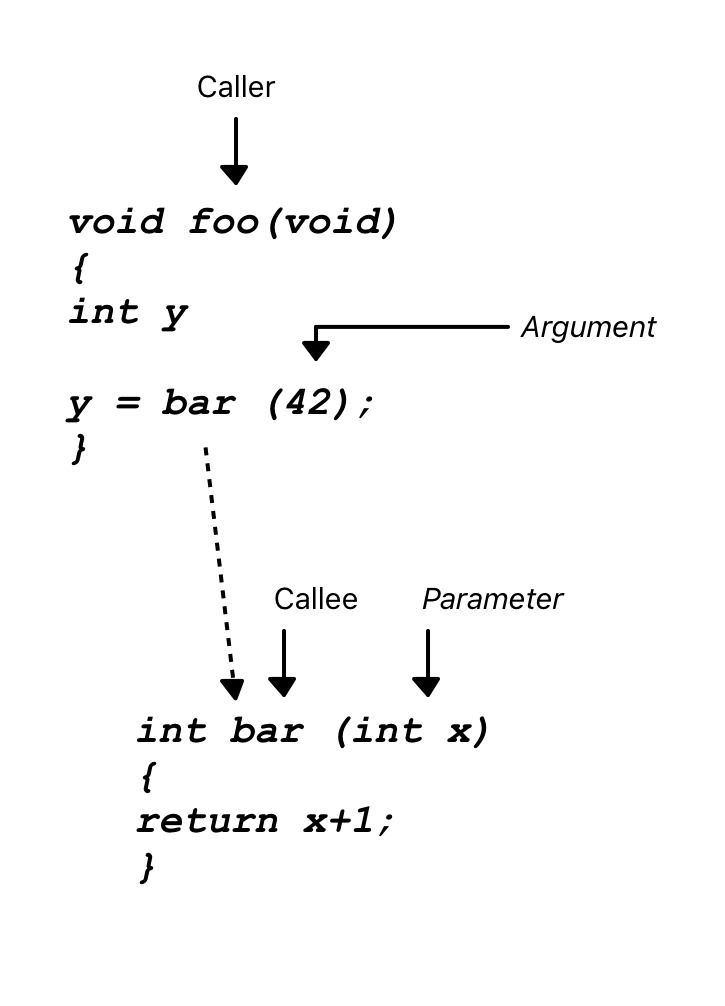
\includegraphics[width=0.4\textwidth]{callee.jpg}
\caption{Caller-callee argument-parameter}
\label{figure:callee}
\end{figure}

Figure \ref{figure:callee} shows the function \textit{foo(...)} invoking \textit{bar(...)}. \textit{foo(...)} is called the \textit{caller} \index{caller} and \textit{bar(...)} is called the \textit{callee} \index{callee}. The argument 42 is passed into the callee function as a parameter. \index{parameters} \index{arguments} Parameter \textit{x} is assigned the value 42. Within the callee function the resulting return number becomes 43 (=\textit{x+1}). We can see that \textit{bar(...)} is the last function called. It calls no other functions. This function is given a special name, it is called a \textit{leaf function}, as-in the end node of the tree. \index{leaf function}

This short section covers 80\% of the C Programming Language. The rest of the language is all about the details and corner cases.






\newpage
\section{Comments}

Before we go any further, we should get familiar with the different types of comments \index{comments} available in C. C has two types of comments, namely block and line.  \index{comment block}\index{comment line}Let's take the \textit{hellow2.c} example and insert both block and line comments. Comments are extremely important to explain why particular decisions are made. If we return 6 months later, the comments should help make the code more understandable. In other words, the code plus comments must provide enough basic information to explain the purpose of the code.\\

\begin{lstlisting}[language=C,showstringspaces=false,caption={File hellow2.c, with block and line comments},captionpos=b]
 1 #include <stdio.h>
 2
 3 /* Line 1
 4    Line 2
 5    Line 3 This is a block comment and it goes on to multiple lines
 6    Line 4 */
 7 
 8 int main(void) // this is a single comment line 
 9 {
10 printf("Hello World\n");
11
12 return 0;
13 }
\end{lstlisting}

Block comments start with /* and end with */. They allow for multiple line comments to be embedded into the source code and they are useful when describing more complex concepts. You can see a block comment shown on lines:3-6. The compiler ignores everything in-between the /* and */, so even obsolete or discarded code can placed within the comments. 

By contrast, a line comment simply starts with "//" to the End-Of-Line (EOL). A useful feature if you want to write short comments, as shown in the example on line:8. This type of comment was adopted from the C++ language.

As a good practice it is recommended that you create a standard comment block that explains what a function is designed to achieve before writing the code. This is useful when attempting to build larger projects. This standard comment block describes what the routine is supposed to do, providing more details on the parameters passed into the function as well as the return type with the result. 

An example is shown in listing \ref{stdcommblock} providing the function NAME, function DESCRIPTION, input PARAMETERS, RETURN type, EXAMPLE on how-to-use, and finally a NOTES section covering the side effects. C functions are not pure mathematical functions but functions or procedures that can achieve many objectives including side effects. 

In this book we have not included full comments to save space but in a professional or academic setting we would recommend adopting this approach.\\
  
\begin{lstlisting}[language=C,caption={Example function header comment},captionpos=b,label=stdcommblock]
/*
 * NAME
 *
 *  add
 *
 * DESCRIPTION
 *
 *  This routine adds two integers together and returns the result as an integer. 
 *
 * PARAMETERS
 *
 *  int a - first integer 
 *  int b - second integer
 *
 * RETURN
 *
 *  integer
 *
 * EXAMPLE
 *
 *  fortytwo = add(40,2);
 *
 *    if (fortytwo!=42)
 *    { 
 *    printf("fortytwo not equal to 42 \n");
 *    return -1;
 *    }
 *
 * NOTES
 *
 *  simple routine, no side effect
 *
 */
\end{lstlisting}


Finally a general rule when writing C code: make the functions as short as possible. Longer functions are more complex and harder to debug or optimize. Long functions add complexity making it easier to accidentally inject unanticipated mistakes. The general rule-of-thumb for function length is no longer than 100 lines (roughly a screen full). If a function is too long then it is probably better to deconstruct it into smaller pieces. Files longer than 500 lines, or perhaps 1000 lines, are ripe for some form of structural investment.\\


 
\newpage
\section{Source Files} \label{sourcefiles}

The C language has two important file types, namely .c and .h. The .h files are headers \index{.h header files} \index{.c source files} or definitions and the .c files are source code implementations. The .c and .h file types are more stylistic in that they can be used in all sorts of interesting ways. The standard and recommended method is to treat .h files as definitions and .c files as implementation. A good practice for header files is to include the preprocessor directives \#ifndef FILENAME\_H\_ \#define FILENAME\_H\_, to avoid multiple header inclusions. More on this later when we start to discuss large projects and header inclusion headaches.

A C project is made up of a number of .h and .c files. And in essence the header definition .h files express the software contract which is exported and used by the other parts of the project. Or alternatively use as a method to export functions for use by other parts of the program.

Lets walk through a simple example, take the function \textit{add(...)} which has two input parameters, called \textit{int a} and \textit{int b} respectively (see line:1 in listing \ref{addbody}). Both are of type \textit{int}. These parameters are used in the calculation. Return type is also \textit{int} (integer). In the body of the function (denoted by the curly brackets) we carry out the addition and return the result, as shown on line:3.\\

\begin{lstlisting}[language=C,showstringspaces=false,caption={File add.c, add two integers},captionpos=b,label=addbody]
 1 int add(int a, int b)
 2 {
 3 return a+b; // add two numbers together
 4 }
\end{lstlisting}

Nothing complicated, the code is fairly self-explanatory. Say we save this function to a file called add.c. Now if we want to make the \textit{main(...)} function slightly more complicated by allowing the \textit{add(...)} function to be invoked we simply insert it into the function body as shown on line:7 in listing \ref{helloworld2}. 

\begin{lstlisting}[language=C,showstringspaces=false,caption={File hellow2.c, invokes add(...) function},captionpos=b,label=helloworld2]
 1 #include <stdio.h>
 2
 3 int main(void)
 4 {
 5 int result;
 6
 7 result=add(1,1);
 8
 9 printf("Hello World, number returned is %d\n",result);
10
11 return 0;
12 }
\end{lstlisting}

Note in this example you can also see a variation of \textit{printf(...)} which takes the variable \textit{result} and outputs the contents to the console. The output location is designated by \%d which symbolizes where the number will appear in the output string. In this case the number will appear at the end of the line (i.e. just before the newline).\\

If we compile the code now, the C compiler will complain that it doesn't recognize the function \textit{add(...)} on line:7. This means somehow we need to provide a method to define the \textit{add(...)} function so that the compiler can recognize the function call name. This is achieved using a header .h file that describes the function definition. Lets create a header file called \textit{add.h}. And within this file we provide a definition of the function. This function definition is called a function prototype. The compiler processes source code sequentially so a function must be defined before use, either by prototype or with the function implementation itself. This would require the \textit{add(...)} function body to be in the same file, as the caller has to be physically located above the first use.

\begin{lstlisting}[language=C,caption={File add.h, header file},captionpos=b]  
int add (int a, int b);
\end{lstlisting}

In listing 6 we have created a function prototype that describes the input-output interface to the \textit{add(...)} function but does not contain the implementation, this code is in the \textit{add.c} file. Unfortunately \textit{hellow2.c} still refuses to compile, so we have to insert another include which loads the definition file. In this case the definition file \textit{add.h}, as shown on line:6 in listing \ref{helloworldcomplete}.\\

\begin{lstlisting}[language=C,showstringspaces=false,caption={File hellow3.c, complete},captionpos=b,label=helloworldcomplete]   
 1 /*
 2  * IMPORT
 3  */
 4
 5 #include <stdio.h>
 6 #include "add.h"
 7
 8 /*
 9  * BODY
10  */
11
12 int main(void)
13 {
14 int result;
15
16 result = add(1,1); // add 1+1
17
18 printf("Hello World, number returned is %d\n",result);
19
20 return 0;
21 }

OUTPUT

Hello World, number returned is 2
$

\end{lstlisting}
 
There is a slight difference in the two includes used on line:5 and line:6. The standard library inclusion is denoted by \textless{library name.h}\textgreater \, as seen on line:5, whereas the local library inclusion is denoted by "library name.h" on line:6. The different methods is used by the compiler to look along particular file paths. For local include files the compiler searches the current directory /. whereas the standard library search path will be \textit{/usr/local/lib}. 

We can also explicitly provide the complete file path to a header file e.g. "myheaders/example.h".

One extra trick is to stop the same header files from being included multiple times. This is achieved by adding some preprocessor directives, as shown in listing \ref{multiple}. This technique is simple and effective. The technique is to check for a specific macro define. If the macro define has previously been defined then the header is ignored. If the macro define is not defined then the header is loaded.\\

\begin{lstlisting}[language=C,caption={File add.h, full header file},captionpos=b,label=multiple]  
#ifndef ADD_H_
#define ADD_H_

// Function Prototypes

int add(int a,int b);

#endif
\end{lstlisting}

 This is useful when building larger projects. It is quite easy to accidentally include the same .h file multiple times and confuse the compiler. This technique removes the problem of loading the same header file multiple times.\\


\newpage
\section{Building} 

To execute a C program we first have to compile the source code into object files. If there are no issues with the compilation stage the object files can then be linked together to create an executable file. The executable file can then be called from a command line and run. The procedure is shown in figure \ref{compile}. 

\begin{figure}[H]
\centerline{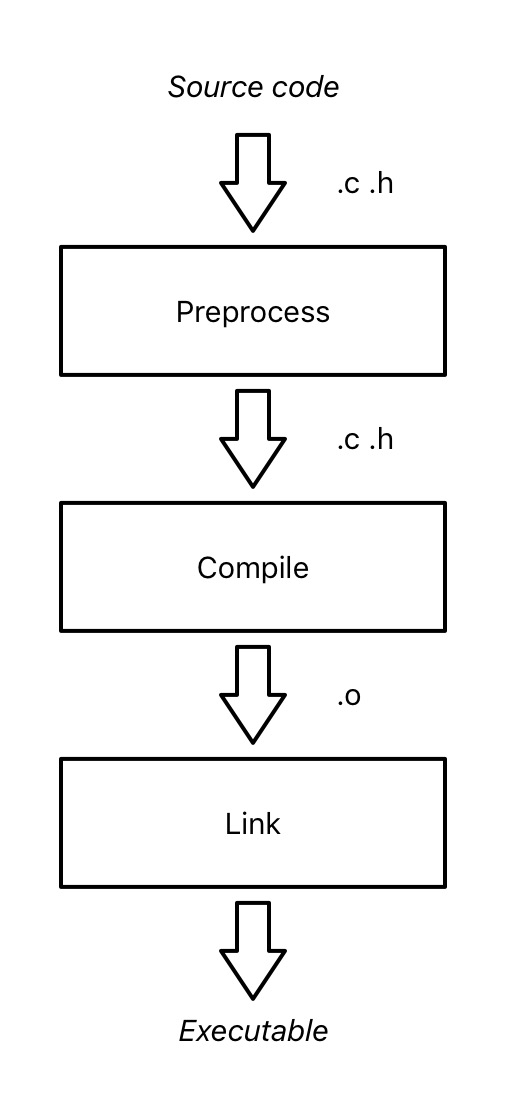
\includegraphics[width=0.3\textwidth]{cycle.jpg}}
\caption{Compile-link process}
\label{compile}
\end{figure}

As already discussed in section \ref{sourcefiles}, a C project is made up of .c and .h files (as well as .s assembler files). When these files are compiled an object or simply a .o file is created. .o files are in a format called ELF (Executable and Linkable Format). The ELF object format is a binary linkable format that cannot be simply read using a standard text editor but can be read by the linker. These types of files are collectively called binary files.

 If there are no errors the .o files can be linked together creating an executable file. The executable file is in what is called an ELF executable format. The ELF executable format contains a standard header at the beginning of the file. This information is used by the Operating System to discover the load address, image type, etc.. The image type defines the hardware architecture that is to be executed. For example, execute type can be AArch64 or x86-64. If an attempt is made to execute on the wrong hardware architecture the Operating System will complain declaring the executable architecture is incompatible.
 
The compiler converts .c and .h files into .o files. For Linux the standard compiler is the GNU C Compiler which is invoked by \textit{cc}, \textit{gcc} or by the more specific full name \textit{arch-elf-gcc}. Note \textit{arch-elf-gcc} is used for cross-compilation, as-in compiling on one architecture to produce binaries for another architecture. For example a typical setup involves developing on a desktop computer and transfer the images to an embedded devices. Cross-compilation is a very common technique with embedded developers. 

\subsection{Compile to executable}

To build the \textit{Hello World} example into an executable, we simply follow the path shown in figure \ref{compile}. This is achieved by compiling the example code \textit{hellow.c} with no options. The compiler will automatically invoke the preprocessor, compiler and finally linker. This will produce an executable image called \textit{a.out}. If the program doesn't include a \textit{main(...)} entry point the linker will throw out an error.\\

\begin{lstlisting}[language=bash,showstringspaces=false,caption={Example compile and execute},captionpos=b,label=simpleb]
 1 $ cc hellow.c
 2 $ ./a.out
 3 Hello World
 4 $ 	
\end{lstlisting}

Listing \ref{simpleb} shows the easiest method to build an executable. Next we want to compile same example but with a specific executable name rather than the generic \textit{a.out}. To achieve this we use the \textit{-o} option.\\ 

\begin{lstlisting}[language=bash,showstringspaces=false,caption={Example compiling and specifying the execution name},captionpos=b,label=hello]
 1 $ cc -o hellow hellow1.c
 2 $ ./hellow
 3 Hello World
 4 $ 	
\end{lstlisting}

Listing \ref{hello} uses the same procedure as the previous example but we build an executable named \textit{hellow} as shown on line:2.

\subsection{Compile to object file}

For larger projects it may be necessary to split the creation of object files and the linking of a final executable. This involves building the object files first before linking them together. This is achieved using the option \textit{-c}. This option instructs the compiler to produce .o files only and not carry out the final linking of an executable image.\\

\begin{lstlisting}[language=bash,showstringspaces=false,caption={Example compiling only, producing object files},captionpos=b,label=linkonly]
 1 $ cc -c hellow1.c
 2 $ ls *.o
 3 hellow.o
 4 $ 	
\end{lstlisting}

Listing \ref{linkonly} shows the link only procedure, with line:1 creating the object file \textit{hellow.o}.

\subsection{Compile with multiple files}

Until now we have exclusively built executables using a single source file but most projects involve multiple files. To build an executable from two or more files we have a slightly different procedure. Listing \ref{multibuild} takes \textit{hellow2.c} and \textit{add.c} respectively and compiles them together, as shown on line:1. Directly creating \textit{a.out} executable file.\\

\begin{lstlisting}[language=bash,showstringspaces=false,caption={Example compiling and linking multiple files},captionpos=b,label=multibuild]
 1 $ cc hellow2.c add.c
 2 $ ./a.out
 3 Hello World, number returned is 2
 4 $ 	
\end{lstlisting}

The next example in listing \ref{multibuild2} takes a mixture of .c and .o files to build an executable. Line:1 shows the \textit{add.o} being created. Line:2 shows \textit{hellow2.c} file being compiled with the previously formed \textit{add.o} file to create an executable called \textit{hello2}.\\

\begin{lstlisting}[language=bash,showstringspaces=false,caption={Example compiling and linking multiple files with a specified execution name},captionpos=b,label=multibuild2]
 1 $ cc -c add.c
 2 $ cc -o hello2 hellow2.c add.o
 3 $ ./hello2 
 4 Hello World, number returned is 2
 5 $ 	
\end{lstlisting}

Line:4 shows the result of adding 1 and 1 together and outputting the result to the console.

\subsection{Libraries}

\index{building libraries}
\index{library}

A library is a grouping of related function calls placed into a single file. There are two types of libraries, namely \textit{shared} and \textit{static}. We will leave the shared library for further exploration since this is more Operating System specific. The static library will be explained in more detail here. A static library is a file containing one or more object files. As already described, an object file contains a set of compiled function calls. A library can then be linked to a image to form an executable. They are useful when the same functionality is required by multiple programs.\\  

\begin{lstlisting}[language=bash,showstringspaces=false,caption={File hellow3.c, build library},captionpos=b,label=library]
 1  $ cc -c add.c sub.c
 2  $ ar cvq simple_lib.a add.o sub.o
 3  q - add.o
 4  q - sub.o
 5  $ cc hello3.c simple_lib.a
 6  $ ./a.out
 7  a+b=30
 8  a-b=10 	
\end{lstlisting}

Listing \ref{library} shows how to build a simple library. Line:2 uses the \textit{ar} util tool (also known as the archive tool) to create the library \textit{simple\_lib.a}. This library can then be used to create an executable, as shown on line:5. 

\subsection{Makefile}

\index{makefile}

Make is a powerful build tool. It is used to build larger projects. There are a number of \textit{make} like alternatives that are worth exploring but \textit{make} is useful since it checks for dependencies which allows for incremental builds.

An incremental build is one where only the source files that are newer than the executable are re-compiled. This means not all of the files are re-compiled each time we want to create an executable. This saves a lot of time when dealing with larger projects.\\

\begin{lstlisting}[language=bash,showstringspaces=false,caption={File Makefile, build a program called hello},captionpos=b,label=makefile]
 1 hello : hellow2.o add.o 
 2 		cc -o hello hellow2.o add.o
 3
 4 hellow2.o : hellow2.c add.h
 5  	cc -c hellow2.c
 6 
 7 add.o : add.c add.h 
 8 		cc -c add.c
 9
10 clean :
11 		rm hello hellow2.o add.o

INTERACTION

12 $ make clean
13 rm hello hellow2.o add.o
14 $ make
15 cc -c helloworld2.c
16 cc -c add.c
17 cc -o hello hellow2.o add.o
18 $ ./hello
19 Hello World, number returned is 2
20 $ nano add.c  
21 $ make
22 cc -c add.c
23 cc -o hello hellow2.o add.o
24 $ 
\end{lstlisting}
   
Listing \ref{makefile} shows a simple \textit{make} project. The project builds an executable called \textit{hello} line:1. The dependencies for \textit{hello} are \textit{hellow2.o} and \textit{add.o} respectively. Line:2 shows the final command to build \textit{hello}. The makefile itself is called \textit{Makefile} in the filing system. It can have other names but by default the \textit{make} util looks for that file name unless otherwise directed.

Lines:4:7 shows the dependencies for building specific object files. Lines:5:8 show the compiler command to build the object files. Line:2 is the finished project compiler command to build the executable. Finally line:1 are the dependencies for the executable.


Lines:10:11 specify the \textit{clean} option when \textit{make clean} is typed in on the console. Line:11 removes all the old object files and the current executable leaving just source code.

We have now covered the different aspects of compiling, from a simple compilation of one file to building of a Makefile for more complex projects. Other areas worth exploring, compiling for debug and compiling with assembly files.



      
\newpage
\section{Preprocessor} \label{preprocessor}

Preprocessor is exactly what it sounds like, it preprocesses the C source files before compilation. Warning, overuse of the preprocessor directives can make source code confusing and difficult to read. The preprocessor is an extension of the build and is not technically part of the C language. More modern programming languages do not include this feature.

\subsection{\#include}

\index{\#include}

\textit{\#include} imports a file. Essentially there are two header file types, standard and user. Standard header files require a \textless header file.h\textgreater\space and user header files require "header file.h". The standard header files are in specific shared library directories, whereas the user files are searched locally. A hardcoded file path can also be used.

\subsection{\#define}

\index{\#define}

This directive allows for a macro name to be defined. Macros are used extensively throughout C projects. The preprocessor takes the macro name and replaces it with whatever you have defined as the macro to be. It only replaces macro names forward of the definition location, it does not carry out a global find and replace.

\begin{lstlisting}[language=C,showstringspaces=false, caption={File macro1.c, LOG macro},captionpos=b,label=macro1]

 1 #include <stdio.h>
 2 
 3 #define ANGLE 34
 4 #define LOG(s)   printf("LOG:%s\n",s)
 5 
 6 
 7 int main(void)
 8 {
 9 LOG(" enter: main");
10 
11   printf("Hello World, angle %d\n",ANGLE);
12 
13 LOG(" exit: main\n");
14 return 0;
15 }

INTERACTION

$ cc macro1.c
$ ./a.out
LOG: enter: main
Hello World, angle 34
LOG: exit: main
$

\end{lstlisting}

Listing \ref{macro1} shows a simple and a more complex define. The first simple \textit{\#define} sets \textit{ANGLE} to 34. Every occurrence of ANGLE within the source code gets converted to 34.. The second \textit{\#define} \textit{LOG(s)} takes an argument and inserts that argument into a \textit{printf(...)} function call.

\subsection{\#undef}

\index{\#undef}

This directive is the opposite to \textit{\#define}, it simply undoes an already defined macro. If a macro name has been set it can be unset. This is useful when redefining a macro, undef removes the macro and allows it to be defined again.

\subsection{\#ifdef}

\index{\#ifdef}

The \textit{\#ifdef} directive is used to control flow within the source code. For example, placing a file in DEBUG mode. This is useful if there is a need to have more diagnostic information, otherwise the program compiles normally. In essence \textit{\#ifdef} provides different compile output options depending upon the requirement.

\begin{lstlisting}[language=C,showstringspaces=false, caption={File macro2.c, \#ifdef DEBUG macro},captionpos=b,label=macro2]

 1 #include <stdio.h>
 2 #include <time.h>
 3 #include <unistd.h>
 4 
 5 // #define DEBUG 
 6 
 7 int main(void)
 8 {
 9 #ifdef DEBUG
10 time_t currtime = time(NULL);
11 #endif
12 
13   printf("Hello World\n");
14   sleep(3); // wait 3 seconds
15 
16 #ifdef DEBUG
17 printf("debug: time take: %ld\n",time(NULL)-currtime);
18 #endif
19 
20 return 0;
21 }

INTERACTION

$ cc -DDEBUG macro2.c
$ ./a.out
Hello World
debug: time take: 3
$ cc macro2.c
$ ./a.out
Hello World
$

\end{lstlisting}


Listing \ref{macro2} shows a \textit{\#ifdef} example. When the macro DEBUG is defined the lines:10:17 becomes part of the source code otherwise both lines are ignored by the compiler. MACROS can be hardcoded or passed into the source via the compiler using the \textit{-D} compiler directive, as shown in the INTERACTION part. 

\subsection{\#ifndef}

\index{\#ifndef}

The \textit{\#ifndef} directive is used to control flow within the source code. For example, by placing a file in NODEBUG mode diagnostic information is limited otherwise the program by default runs in full DEBUG or diagnostic mode.

\begin{lstlisting}[language=C,showstringspaces=false, caption={File macro3.c, \#ifndef NODEBUG macro},captionpos=b,label=macro3]

 1 #include <stdio.h>
 2 #include <time.h>
 3 #include <unistd.h>
 4 
 5 int main(void)
 6 {
 7 #ifndef NODEBUG
 8 time_t currtime = time(NULL);
 9 #endif
10 
11   printf("Hello World\n");
12   sleep(3); // wait 3 seconds
13 
14 #ifndef NODEBUG
15 printf("debug: time take: %ld\n",time(NULL)-currtime);
16 #endif
17 
18 return 0;
19 }

INTERACTION 

$ cc macro3.c
$ ./a.out
Hello World
debug: time take: 3
$ 

\end{lstlisting}

Listing \ref{macro3} shows an opposite example to \textit{\#ifdef}. When the macro NODEBUG is defined lines:8:15 don't become part of the source code otherwise by default the lines become part of the source code.

\subsection{\#if, \#elif and \#else}

\index{\#if}
\index{\#elif}
\index{\#else}

These directives provide a more traditional decision making control flow for the preprocessor.

\begin{lstlisting}[language=C,showstringspaces=false, caption={File macro4.c, using \#define macro},captionpos=b,label=macro4]

 1 #include <stdio.h>
 2 #include <time.h>
 3 #include <unistd.h>
 4 
 5 #define BUFSIZE 42
 6 
 7 int main(void)
 8 {
 9 int margin;
10 
11 #if defined BUFSIZE && BUFSIZE > 1024
12 margin = 2;
13 #elif BUFSIZE > 624
14 margin = 1;
15 #else
16 margin = 0;
17 #endif
18 
19 printf("margin=%d\n",margin);
20 return 0;
21 }
22 
23 

INTERACTION

$ cc macro4.c
$ ./a.out
margin=0
$ 

\end{lstlisting}


The listing \ref{macro4} shows an example using the \textit{\#if}, \textit{\#elif} and \textit{\#else} preprocessor directives. The example sets the BUFSIZE macro to 42. If the BUFSIZE macro is larger than 1024 then the \textit{margin} variable is assigned the value 2 on line:12. If BUFSIZE is larger than 624 and less than 1025 then the \textit{margin} variable is assigned the value 1 on line:14, otherwise \textit{margin} is assigned the value 0. In the example the BUFSIZE macro is set to 42 which means the \textit{margin} becomes 0 on line:16.

\subsection{\#error}

\index{\#error}

The \textit{\#error} directive halts compilation with an error message.

\begin{lstlisting}[language=C,showstringspaces=false, caption={File macro5.c, using \#if, \#else, \#error and \#endif},captionpos=b,label=macro5]

 1 #include <stdio.h>
 2 #include <time.h>
 3 #include <unistd.h>
 4 
 5 #define BUFSIZE 700
 6 
 7 int main(void)
 8 {
 9 int margin;
10 
11 #if defined BUFSIZE && BUFSIZE > 1024
12 margin = 2;
13 #elif BUFSIZE > 624
14 #error "BUFSIZE is wrong size"
15 #else
16 margin = 0;
17 #endif
18 
19 printf("margin=%d\n",margin);
20 return 0;
21 }

INTERACTION 

$ cc macro5.c
macro5.c:14:3: error: "BUFSIZE is wrong size"
#error "BUFSIZE is wrong size"
  ^
1 error generated.
$  

\end{lstlisting}

Listing \ref{macro5} shows an example of \textit{\#error}. The \textit{\#error} on line:14 forces a halt of compilation. The BUFSIZE macro is set to 700 on line:5 and it subsequently causes an compilation error on line:14.

\subsection{\#pragma}

\index{\#pragma}


Sends additional advice back to the C compiler. It is dependent upon the the compiler being used. \textit{\#pragma} gives a hint to the compiler, for example \textit{ignore warnings} or \textit{don't optimize}. 

 

 
\newpage
\section{Standard C Libraries}

The C Programming Language doesn't just include the core language but also includes supporting libraries. These libraries allow C source code to be relatively portable between hardware architectures and Operating Systems. The use of libraries also removes the need to duplicate or re-invent particular features. 

The libraries reduce the amount of overall testing since the standard libraries have already been vigorously tested before being released. As previously mentioned, C was originally developed in 1972 and since that time it has gone through a number of major language and library revisions. The most notable recent revisions are shown in table \ref{table:revisions}.\\ 

\index{NA1}
\index{C11}
\index{C99}

\begin{table*}[ht]
\centering
  \begin{tabular}{ | c | c | l |}
    \hline
    SHORT NAME & YEAR & DESCRIPTION \\ \hline
    NA1 & 1995 & ISO/AMD1 9899:1995  \\ \hline
    C99 & 1999 & ISO/IEC 9899:1999  \\ \hline
    C11 & 2011 & ISO/IEC 9899:2011  \\ \hline  
  \end{tabular}
\caption{Revision history}
\label{table:revisions}
\end{table*}

Just taking one library example, the \textit{stdbool.h} library. This library was introduced in the C99 revision. This was 27 years after the language first appeared. \textit{stdbool.h} standardizes the boolean datatype. For more information see section \ref{stdbool} on page \pageref{stdbool}. 

\clearpage

Table \ref{Table:StandardLibraries} shows the standard libraries provided with the C Programming Language. It is worth having a rough understanding of the library landscape. To help the learning curve the USEFUL column marks a subset of libraries to review first. It should be noted that the libraries provided are just the standard C libraries. There are other common library standards used with C. As an example the POSIX standard. POSIX introduces a number of important features found in Unix based Operating Systems.\\

\index{POSIX}

\begin{table}
\centering
  \begin{tabular}{ | c | l | c | l |}
    \hline
    USEFUL & NAME & REVISION & DESCRIPTION \\ \hline
    x          & assert.h &  & assert macro \\ \hline
               & complex.h & C99 & handles complex numbers \\ \hline
    x		   & ctype.h & & character manipulation e.g. upper to lower \\ \hline
    x          & errno.h &  & error types \\ \hline
               & fenv.h & C99 & control floating point environment \\ \hline
               & float.h &  & macro floating point constants \\ \hline
               & inttypes.h & C99 & exact width types \\ \hline
               & iso646.h & NA1 & ISO 646 character set \\ \hline
               & limits.h &  & macros constants for integers \\ \hline
               & locale.h &  & localization functions \\ \hline
    x          & math.h &  & common maths functions \\ \hline
               & setjmp.h &  & non local jumps \\ \hline
               & signal.h &  & signal handling functions \\ \hline
               & stdalign.h &  C11 & align objects \\ \hline
               & stdarg &  & varying number of arguments \\ \hline
               & stdatomic.h & C11 & atomic operations \\ \hline
    x          & stdbool.h & C99 & boolean datatype \\ \hline
               & stddef.h &  & useful types and macros \\ \hline
    x          & stdint.h & C99 & width integer types \\ \hline
    x          & stdio.h &  & core input/output functions \\ \hline
    x          & stdlib.h &  & misc. useful functions \\ \hline
               & stdmoreturn.h & C11 & non-returning functions \\ \hline
    x          & string.h &  & string handling functions \\ \hline
               & tgmath.h & C99 & type-generic mathematical functions \\ \hline
               & threads.h & C11 & thread handling \\ \hline
    x		   & time.h &  & date and time functions \\ \hline
               & uchar.h & C11 & UNICODE characters \\ \hline
               & wchar.h & NA1 & wide string handling functions \\ \hline
               & wctype.h & NA1 & useful functions for wide characters \\ \hline   
  \end{tabular}
\caption{Standard C libraries}
\label{Table:StandardLibraries}
\end{table}

If we plan to use many libraries, it is worth creating a single header file that incorporates all the header files we plan to use. This way if we want to use those libraries in our project all we have to do is include a single file. This can save a lot of time and pain.

\begin{lstlisting}[language=C,caption={File all.h, universal header file},captionpos=b,label=headers]  

#ifndef ALL_H
#define ALL_H

// Standard C Libraries

#include <stdio.h>
#include <stdlib.h>
#include <string.h>
#include <stdbool.h>
#include <stdint.h>

// User Header Files

#include "add.h"
#include "sub.h"

#endif
\end{lstlisting}

Listing \ref{headers}, shows a header file called \textit{all.h}. This header file brings in the header file for a number of popular libraries i.e. \textit{stdio.h},\textit{stdlib.h},\textit{string.h},\textit{stdbool.h} and \textit{stdint.h}. As well as a number of user local headers i.e. \textit{add.h} and \textit{sub.h}. Each .c implementation file can simply include the \textit{all.h} header. This header will bring in all the necessary libraries required. This can save a lot of time in more complex projects.


\newpage
\section{Variables} \label{avari}

The C Programming Language has a number of basic builtin variable types as well as some more complex types brought in via standard libraries. This section covers both the builtin types and some of the more common library types used in Embedded Systems. 

\subsection{Builtin basic types}

These are the common variable types found extensively in C source code. The table is not exhaustive but provides a core set of types. It is always worth spending a little time understanding the variable type ranges as they can differ depending upon the compiler being used and the hardware architecture being targeted. In C, all variables used have to first be declared.

\begin{table}[H]
  \centering
  \begin{tabular}{ | l | l | l | l |}
    \hline
    TYPE & STORAGE & FORMAT & RANGE \\ \hline
    char & 1 byte & 1 signed bit + 7 bits & -128 to +127 \\ \hline
    unsigned char & 1 byte & 8 bits & 0 to 255 \\ \hline
    short & 2 bytes & 1 signed bit + 15 bits & -32,768 to 32,767 \\ \hline
    unsigned short & 2 bytes & 16 bits & 0 to 65,535 \\ \hline
    int & 4 bytes & 1 signed bit + 31 bits & -2,147,483,648 to +2,147,483,647 \\ \hline
    unsigned int & 4 bytes & 32 bit & 0 to 4,294,967,295 \\ \hline
    float & 4 bytes & 6 decimal places & 1.2E-38 to 3.4E+38 \\ \hline
    double & 8 bytes & 15 decimal places & 2.3E-308 to 1.7E+308 \\ 
    \hline
  \end{tabular}
\caption{Basic C types}
\label{ctypes}
\end{table}

\subsection{Loop variables}

A common convention in C is to use short and abbreviated names. This can be seen when scanning C code examples. For instance, it is common to use \textit{'i’}, as in \textit{for (i = 0; i < 10; i++) ...}, in loops as these were lifted at a time when Fortran was a common programming language and had reserved keywords for loop structures.

\subsection{void type} \label{voidtype}

\index{void}

This is a special type called \textit{void}. It is a builtin type with special properties. These properties are context dependent. The three context that \textit{void} operates under are:-

\begin{itemize}
  \item[$\bullet$]  \textbf{Function parameter}: \textit{void} found in the parameter-list means no parameters e.g. \textit{printhello(void);} so a caller function would have \textit{printhello();} i.e. no parameters.
  \item[$\bullet$] \textbf{Return type}: \textit{void} means no return. Extending the previous example \textit{void printhello(void);} this means that the function does not return a value. Note \textit{return;} with no value can be used exit a \textit{void} function. It can be placed anywhere within the function body.  
  \item[$\bullet$] \textbf{Generic pointer}: where the object being pointed to is generic or unknown. We talk about pointers in more detail in section \ref{Pointers}.
\end{itemize}

\subsection{Boolean type}\label{stdbool}

\index{bool} 
\index{stdbool.h}

The boolean type isn't a builtin type in the C language. Boolean is an implied type using either integers or characters. It is now a standard library. Boolean type was introduced in the C99 revision. To use the standard boolean type we have to include the library \textit{stdbool.h}.\\

\begin{lstlisting}[language=C,showstringspaces=false,caption={File bool.c, using the stdbool.h bool type},captionpos=b,label=bool]

 1 #include <stdio.h>
 2 #include <stdbool.h>
 3 
 4 int main(void)
 5 {
 6 bool logic_a = true;
 7 
 8   if (logic_a) 
 9   {
10   printf("logic_a==TRUE\n");
11   }
12   else
13   {
14   printf("logic_a==FALSE\n");
15   }
16   
17 return 0;
18 }

INTERACTION

19 $ cc bool.c
20 $ ./a.out
21 ... logic_a==TRUE
22 $

\end{lstlisting}

Listing \ref{bool} shows an example using \textit{bool} type. The code declares a variable called \textit{logic\_a} that is set to logic value \textit{true} on line:6. The variable is used as an expression on line:8. If expression result in \textit{true} then TRUE is displayed, otherwise FALSE. In the example, \textit{logic\_a} is set to true so TRUE is displayed, as shown on line:21. 

\subsection{Casting to a different type}

Casting allows one type to be transformed (cast) as another type. This is useful when requiring a change, where the original type isn't compatible with either a manipulation operation or output format. Quite often it is used to avoid an error or warning message being thrown out by the compiler.\\

\begin{lstlisting}[language=C,showstringspaces=false,caption={Example casting, char to int},captionpos=b,label=casting]
 1 char y;
 2 int x;
 3  
 4 x = (int) y;
\end{lstlisting}

Listing \ref{casting}, casts the variable \textit{y} of type \textit{char} to \textit{int} on line:4. The cast value is then assigned to variable \textit{x}. A \textit{char} casted to an \textit{int} gives the ASCII value of \textit{char}. This value can now be manipulated as an \textit{int}. It is not recommended to cast unless you are forced to change types. This feature should be used sparingly.  

\subsection{C99 types}

\index{stdint.h}

By including the header file \textless stdint.h\textgreater \, the new integer types will be available which are particularly useful in embedded programming. These new types incorporate the bit size of the type within the name. This is useful when accessing hardware when the type size is important to know. 

For example, the new integer types are defined as \textit{int\{bit size\}\_t} and correspondingly the new unsigned integer types are defined as \textit{uint\{bit size\}\_t}. Where is the \textit{bit size} can be 8, 16, 32 and 64. Table \ref{inttypes} shows a subset of the integer types available with \textit{stdint.h}.

\begin{table}[H]
  \centering
  \begin{tabular}{ | l | l |}
    \hline
    TYPE & FORMAT \\ \hline
    int8\_t & signed 8 bits \\ \hline
    uint8\_t & unsigned 8 bits \\ \hline
    int16\_t & signed 16 bits \\ \hline
    uint16\_t & unsigned 16 bits \\ \hline
    int32\_t & signed 32 bits \\ \hline
    uint32\_t & unsigned 32 bits \\ \hline
  \end{tabular}
  \caption{stdint.h: int types}
  \label{inttypes}
\end{table}

\subsection{Variable scope rules}

Variable scoping is part of every programming language and C is no exception. C variable scoping is relatively straightforward. A variable can be scoped as being global or local. 

\subsubsection{Global scope}

\index{global variable scoping}

A global scoped variable can be accessed from anywhere in the file that they are declared in, and with some additional declaration (see \textit{extern} later) from other files. These variables permanently take up storage; by contrast local variables do not occupy permanent storage unless directed (see section \ref{static}).\\

\begin{lstlisting}[language=C,caption={File global1.c, block scope},captionpos=b,label=global1]
#include <stdio.h>

int x=10, y=20;

int calculate(void)
{
return (x+y);
}

int main(void)
{
printf("answer=%d\n",calculate());
return 0;
}

INTERACTION

$ cc global1.c 
$ ./a.out
answer=30
\end{lstlisting}

Listing \ref{global1} shows two globally scoped variables being declared, namely \textit{x} and \textit{y}. These variables are available throughout the entire \textit{global1.c} file. The function \textit{calculate(...)} makes use of this fact to return the value of \textit{x+y} without having arguments.\\

\newpage

\begin{lstlisting}[language=C,caption={File global2.c, local scope},captionpos=b,label=global2]
#include <stdio.h>

int x=10,y=20;

int calculate(void)
{
int x=4, y=7;

return (x+y);
}

int main(void)
{
printf("answer=%d\n",calculate());
return 0;
}

INTERACTION

$ cc global2.c
$ ./a.out
answer=11
\end{lstlisting}

Listing \ref{global2} shows the \textit{calculate(...)}  function using local variables with exactly the same names as the globally scoped variables. The scoping rules have the local variables taking precedence over the global variables. This means the answer 11 is returned rather than 30. In other words, local variables have higher precedence over global variables.

\subsubsection{Extern scope}

\index{extern}

An \textit{extern} scoped variable is a variable where the storage is contained in another object file. The \textit{extern} keyword is used to inform the compiler that the variable is externally defined and the linker has the task of connecting name and storage location in the final image. The variable still has to be defined correctly so that the compiler can understand the name, type and size.

\begin{lstlisting}[language=C,caption={File variables.c, only contains two variables},captionpos=b,label=variables]

1 int x=10;
2 int y=20;
 
\end{lstlisting}

Listing \ref{variables} shows a file called \textit{variables.c} containing two variables \textit{x} and \textit{y}. The variables are both declared as global so they have permanent storage allocated and they are initialized to 10 and 20 respectively. 

\begin{lstlisting}[language=C,caption={File external.c, extern used to access variables in another file},captionpos=b,label=extern]
 
 1 #include <stdio.h>
 2
 3 extern int x,y; 
 4 
 5 int main(void)
 6 {
 7 printf("answer=%d\n",x+y);
 8 return 0;
10 }

INTERACTION
 
$ cc external.c
Undefined symbols for architecture x86_64:
  "_x", referenced from:
      _main in external-bb0f25.o
  "_y", referenced from:
      _main in external-bb0f25.o
ld: symbol(s) not found for architecture x86_64
$ cc -c variables
$ cc external.c variables.o
$ ./a.out
answer=30
$

\end{lstlisting}


Listing \ref{extern} declares two \textit{extern} variables on line:3, \textit{x} and \textit{y}. These variables are of type \textit{int} and they correspond to the global variables defined in \textit{variables.c}. These variables are then accessed in the body of the \textit{main(...)} function. 

If the \textit{external.c} is compiled separately, as shown in the INTERACTION section, the linker throws out an error message saying \textit{"Undefined Symbols"} but when \textit{variables.o} is added the linker completes the compilation.

\subsubsection{Block scope}

\index{local variable scoping}

A block is identified as being between the curly brackets \{ and \}. Outside of the brackets the variables are not accessible, however inside brackets the variables are accessible including any further nested brackets.\\

\begin{lstlisting}[language=C,caption={File: block1.c, block scope},captionpos=b,label=block1]
int calculate(void)
{
int x=10, y=20;

return (x+y);
}
\end{lstlisting}

Listing \ref{block1} shows a function called \textit{calculate(...)} that declares and assigns the value 10 to \textit{x} and the value 20 to the \textit{y}. Upon return the two variables are summed together to return the value 30. The variables are available throughout the function body but not outside the brackets. Now let's play with the scoping.\\

\begin{lstlisting}[language=C,caption={File block2.c, block scope with error},captionpos=b,label=block2]
 1 int calculate(void)
 2 { // block1
 3   { // block 2
 4   int x=10, y=20;
 5   }
 6   { // block 3
 7   return (x+y);
 8   }
 9 return (x+y);
10 }

INTERACTION

$ cc -c block2.c
block2.c:7:11: error: use of undeclared identifier 'x'
  return (x+y);
          ^
block2.c:7:13: error: use of undeclared identifier 'y'
  return (x+y);
            ^
block2.c:9:9: error: use of undeclared identifier 'x'
return (x+y);
        ^
block2.c:9:11: error: use of undeclared identifier 'y'
return (x+y);
          ^
4 errors generated.
\end{lstlisting}

Listing \ref{block2} shows a violation of the scoping rules. Both variables \textit{x} and \textit{y} are only declared inside block2. Block 3 contains a return statement with the variables with no declaration and block 1 does not declare the variables. The compiler finds 4 violations (2 x number of variables) of the scoping rules. 
 
\begin{lstlisting}[language=C,caption={File block3.c, block nested scoping with error},captionpos=b,label=block3]
 1 int calculate(void)
 2 { // block 1
 3   { // block 2
 4   int x=10, y=20; 
 5     { // block 3 
 6     return (x+y);
 7     }
 8   }
 9 return (x+y);
10 }

INTERACTION

$ cc -c block3.c
block3.c:9:9: error: use of undeclared identifier 'x'
return (x+y);
        ^
block3.c:9:11: error: use of undeclared identifier 'y'
return (x+y);

2 errors generated.
\end{lstlisting}

Listing \ref{block3} shows how the nested scoping rules operates. There are still errors but that only occurs with the variables in the highest block 1. The scope rules allows access to the variables in the nested block 3. 

\subsection{const qualifier}

\index{const variable}

The const qualifier means that a variable will remain constant and can not be modified. This means that a variable remains constant throughout the lifetime of the program.\\

\begin{lstlisting}[language=C,caption={File const.c, const qualifier},captionpos=b,label=const]
 1 #include <stdio.h>
 2 
 3 int main(void)
 4 {
 5 const int i=42;
 6 
 7 i=23;
 8 
 9 return i;
10 }

INTERACTION

$ cc const.c
const.c:7:2: error: cannot assign to variable 'i' with const-qualified type
      'const int'
i=23;
~^
const.c:5:11: note: variable 'i' declared const here
const int i=42;
~~~~~~~~~~^~~~
1 error generated.
$
\end{lstlisting}

Listing \ref{const} actually produces an error but it shows the principle of the \textit{const} qualifier. If you set a variable to \textit{const} it cannot be modified and if there is an attempt to modify the variable the compiler will throw out and error claiming there was an attempt to modify a \textit{const} variable. 

For embedded systems the \textit{const} qualifier indicates that the variable can be placed in read-only memory. This is useful when there are constraints on the size of volatile memory.

\subsection{static qualifier} \label{static}

\index{static variable}

A static qualifier means that a variable will keep its value between invocations. This is slightly different from global variables where the scoping means that the variable is available throughout the code. A static variable remains within its scope.\\

\begin{lstlisting}[language=C,showstringspaces=false,caption={File static.c, static qualifier},captionpos=b,label=unique]
 1 #include <stdio.h>
 2 
 3 int unique_id(void)
 4 {
 5 static int uid = 1762;
 6 
 7 return ++uid;
 8 }
 9 
10 int main(void)
11 {
12 printf("... uid 0 = %d\n",unique_id());
13 printf("... uid 1 = %d\n",unique_id());
14 
15 return 0;
16 }

INTERACTION

17 $ cc static.c
18 $ ./a.out
19 ... uid 0 = 1763
20 ... uid 1 = 1764
21 $
	
\end{lstlisting}

The listing \ref{unique} shows the function \textit{unique\_id(...)} incrementing a \textit{static} variable each time it is invoked. The scope remains the same. The returning value is unique because it is incremented by the value 1 each time. The initial value is 1762. If the \textit{static} qualifier was not present the returned \textit{uid} variable would always remain 1763.

The \textit{static} qualifier can also applied to a function call to restrict the scope of the function to the current file.

\subsection{volatile qualifier}

\index{volatile variable}

The volatile qualifier informs the compiler that a variable may be updated by another entity, either hardware or software. This in effect disables any optimizations or assumptions that a compiler could have considered. Examples, hardware registers, shared variables between interrupts and thread contexts, multiprocessor access to memory contents, DMA, etc..

As mentioned this entity can be either hardware or software. The qualifier is extremely important in embedded systems when accessing hardware registers. A program cannot determine what the value is at any one point in time and the compiler will therefore not carry out any optimizations such as removing further reads. The hardware register can be continuously updating.

C Compilers do not produce the same code and do not guarantee the same responses without the use of qualifiers. It is important to use wisely.

\begin{lstlisting}[language=C,showstringspaces=false,caption={File volatile.c, volatile qualifier},captionpos=b,label=signal]

 1 #include <stdio.h>
 2 #include <stdlib.h>
 3 #include <signal.h>
 4 #include <unistd.h>
 5  
 6 volatile int x=0;
 7  
 8 void signal_handler(int signal_number)
 9 {
10   if (signal_number==SIGINT)
11   {
12   printf("signal SIGINT caught\n");
13   x=x+1;   
14   } 
15 }
16
17 int main(void)
18 {
19   if (signal(SIGINT,signal_handler)==SIG_ERR)
20   {
21   printf("\nproblem catching SIGINT\n");
22   exit(EXIT_FAILURE);
23   }
24   
25  while (x<3) ; 
26 
27 return 0;
28 }

INTERACTION

29 $ ./a.out
30 waiting for 3 ctrl-c key presses
31 ^Csignal SIGINT caught
32 ^Csignal SIGINT caught
33 ^Csignal SIGINT caught
34 3 ctrl-c key presses occurred
35 $

\end{lstlisting}

The code in listing \ref{signal} guarantees the correct response by using the \textit{volatile} qualifier. It shows a program that uses software interrupts to update a variable called \textit{x}. The program starts by going into an endless loop. It only escapes once ctrl-C is pressed three times. If the variable was not given the qualifier \textit{volatile} the program is not guaranteed to exit since the variable may be held in a register which isn't updated.  

\index{callback}
\index{signal(...)}
\index{unistd.h}
\index{signal.h}
\index{SIGINT}

By placing the \textit{volatile} qualifier on the variable the Compiler has been informed that the variable is likely to change without its knowledge. The function \textit{signal(...)} on line:19 creates a callback which is only invoked when crtl-c is pressed. The callback is \textit{signal\_handler(...)} defined on line:8. \textit{SIGINT} identifies which event to attach to for ctrl-C events.

From the output, it can be seen that ctrl-C is pressed three times on line:31:32:33. Each time this happens the value of \textit{x} is incremented by one. When the value reaches three the program terminates, as shown on line:34.


\subsection{Enumeration type}
\index{enum} \index{enumeration}

The enumeration (\textit{enum}) type is used to enumerate data. It is a basic mapping of names to a number sequence e.g. Zero=0,One=1,...,Ten=10. This variable type is particularly useful when expressing a set of known fixed word-number mappings. For instance, the days-of-the-week or months-in-the-year, where it would be useful to have a limited mapping sequence.

\begin{lstlisting}[language=C,showstringspaces=false,caption={File enum.c, enumeration type},captionpos=b,label=enum]

 1 #include <stdio.h>
 2 
 3 enum direction {North,South,West,East};
 4 enum day {Mon=1,Tue,Wed,Thu,Fri,Sat=10,Sun};
 5 
 6 int main(void)
 7 {
 8 enum direction heading;
 9 enum day today;
10 
11 today=Wed;
12 heading=North;
13 
14 printf ("today is %d and moving in %d direction \n",today,heading);
15 
16 return 0;
17 }

INTERACTION

18 $ ./a.out
19 today is 2 and moving in 0 direction 
20 $

\end{lstlisting}

Listing \ref{enum} shows an enumeration example. Line:3 maps the standard compass directions of \textit{North},\textit{South},\textit{West} and \textit{East} to the values of 0,1,2 and 3 respectively. Line:4 maps the days-of-the-week to the values 1,2,3,4,5,10 and 11 respectively. \textit{Mon=1} sets the sequence start to 1, \textit{Tue} become 2 and so on a long the list. By default the sequence starts at 0.

Line:4 also shows two different sequences within the enumeration list. In this example the weekend is identified by the values 10 and 11. This is achieved by setting \textit{Sat=10}, \textit{Sun} then follows with 11. 

The output from the program is shown on line:19, \textit{\{Wed,North\}} are shown to enumerate to the values of 3 (\textit{today}) and 0 (\textit{heading}) respectively.

  
\newpage
\section{Comparators, Operators and Shifts}

These are the core operators used for mathematical manipulation, assignment and comparison. All expressions adhere to the order of operators. Remember maths class or \textit{Please Excuse My Dear Aunt Sally} (PEMDAS) on how mathematical functions are defined, the C language is no different.

\subsection{Comparators} \label{comparisons}

C language includes the following comparators. Comparators are fundamental in making control decision for program flow. The expressions result to either a 1 (true) or 0 (false) in the C language.

\index{==, equal} 
\index{"!=, not equal} 
\index{\textgreater, greater than} 
\index{\textgreater=, greater than or equal} 
\index{\textless=, less than or equal}

\index{comparators}
\index{comparators!==, equal} 
\index{comparators!"!=, not equal} 
\index{comparators!\textgreater, greater than} 
\index{comparators!\textgreater=, greater than or equal} 
\index{comparators!\textless=, less than or equal}

\begin{table*}[ht]
\centering
  \begin{tabular}{ | c | l | c |} 
    \hline
    OPERATOR & DESCRIPTION & EXAMPLE \\ \hline
    == & Equal & a == b  \\ \hline
    != & Not equal & a != b  \\ \hline
    \textgreater & Greater than & a \textgreater b \\ \hline
    \textless & Less than & a \textless b \\ \hline
    \textgreater= & Greater than and equal & a \textgreater= b \\ \hline
    \textless= & Less than and equal & a \textless= b \\ \hline
  \end{tabular}
\caption{Comparators}
\label{table:comparators}
\end{table*}

\subsection{Logic operators}

C language includes the following logical operators. Logical operators work on boolean values. C provides the standard set of logical operators.


\index{\&\&, logical AND} 
\index{\textbar\textbar, logical OR} 
\index{"!, logical NOT} 

\index{logic operators}
\index{logic operators!\&\&, logical AND} 
\index{logic operators!\textbar\textbar, logical OR} 
\index{logic operators!"!, logical NOT} 

\begin{table*}[ht]
\centering
  \begin{tabular}{ | c | l | c |}
    \hline
    OPERATOR & DESCRIPTION & EXAMPLE \\ \hline
    \&\& & Logical AND & a \&\& b  \\ \hline
    \textbar\textbar & Logical OR & a \textbar\textbar \, b \\ \hline
    ! & Logical NOT & !a \\ \hline
  \end{tabular}
\caption{Logic operators}
\label{table:logicops}
\end{table*}

\subsection{Bitwise operators}

C language also includes the following bitwise operators. The bitwise operators are extremely useful when manipulating hardware registers. Hardware registers require bits to be individually controlled. These operators are important for setting and reading individual bits in hardware registers.

\index{\&, bitwise AND} 
\index{\textbar, bitwise OR} 
\index{\char`\~, bitwise NOT} 
\index{\char`\^,bitwise XOR} 
\index{\textgreater\textgreater, bitwise shift left}
\index{\textless\textless, bitwise shift right}

\index{bitwise operators}
\index{bitwise operators!\&, bitwise AND} 
\index{bitwise operators!\textbar, bitwise OR} 
\index{bitwise operators!\char`\~, bitwise NOT} 
\index{bitwise operators!\char`\^,bitwise XOR} 
\index{bitwise operators!\textgreater\textgreater, bitwise shift left}
\index{bitwise operators!\textless\textless, bitwise shift right}

\begin{table*}[ht]
\centering
  \begin{tabular}{ | c | l | c |}
    \hline
    OPERATOR & DESCRIPTION & EXAMPLE \\ \hline
    \& & Bitwise AND & a \& b  \\ \hline
    \textbar & Bitwise OR & a \textbar \, b \\ \hline
    \char`\~ & Bitwise NOT & \char`\~a \\ \hline
    \char`\^ & Bitwise XOR & a \char`\^ \, b \\ \hline
     \textgreater\textgreater & Bitwise Shift Left & a \textgreater\textgreater \,  3 \\ \hline
     \textless\textless & Bitwise Shift Right & a \textless\textless \, 3 \\ \hline     
  \end{tabular}
\caption{Bitwise operators}
\label{table:bitwiseops}
\end{table*}

\subsection{Arithmetic operators}

C language includes the following arithmetic operators. Arithmetic operators provide the necessary methods to build mathematical equations.

\index{*, multiply}
\index{+, addition}
\index{-, subtraction}
\index{/, division}
\index{\%, modulo}
\index{++, increment pre/post}
\index{-\,-, decrement pre/post}

\index{arithmetic operators}
\index{arithmetic operators!*, multiply}
\index{arithmetic operators!+, addition}
\index{arithmetic operators!-, subtraction}
\index{arithmetic operators!/, division}
\index{arithmetic operators!\%, modulo}
\index{arithmetic operators!++, increment pre/post}
\index{arithmetic operators!-\,-, decrement pre/post}

\begin{table*}[ht]
\centering
  \begin{tabular}{ | c | l | c |}
    \hline
    OPERATOR & DESCRIPTION & EXAMPLE \\ \hline
    * & Arithmetic multiply & a * b  \\ \hline
    + & Arithmetic addition & a + b \\ \hline
    - & Arithmetic subtraction & a - b \\ \hline
    / & Arithmetic divide & a / b  \\ \hline
    \% & Modulo & a \% b \\ \hline
    ++ & Increment pre or post & ++a; or a++; \\ \hline
    -\,- & Decrement pre or post & -\,-a; or a-\,-; \\ \hline
  \end{tabular}
\caption{Arithmetic operators}
\label{table:arithmeticops}
\end{table*}

\subsection{Compound assignment operators}

Compound assignment operators are the operators which are used to update variable contents.

\index{=, assignment}
\index{+=, addition assignment}
\index{-=, subtraction assignment}
\index{*=, division assignment}
\index{\&=, bitwise AND assignment}
\index{\textbar=, bitwise OR assignment}
\index{\char`\^=, bitwise XOR assignment}
\index{\%=, modulo assignment}
\index{\textgreater\textgreater=, bitwise right shift assignment}
\index{\textless\textless=, bitwise left shift assignment}

\index{compound operators}
\index{compound operators!=, assignment}
\index{compound operators!+=, addition assignment}
\index{compound operators!-=, subtraction assignment}
\index{compound operators!*=, division assignment}
\index{compound operators!\&=, bitwise AND assignment}
\index{compound operators!\textbar=, bitwise OR assignment}
\index{compound operators!\char`\^=, bitwise XOR assignment}
\index{compound operators!\%=, modulo assignment}
\index{compound operators!\textgreater\textgreater=, bitwise right shift assignment}
\index{compound operators!\textless\textless=, bitwise left shift assignment}

\begin{table*}[ht]
\centering
  \begin{tabular}{ | c | l | c |}
    \hline
    OPERATOR & DESCRIPTION & EXAMPLE \\ \hline
    =  & Assignment & a = b; \\ \hline
    += & Addition assignment & a += b;  \\ \hline
    -= & Subtraction assignment & a -= b; \\ \hline
    *= & Multiply assignment & a *= b; \\ \hline
    /= & Division assignment & a /= b; \\ \hline
    \%= & Modulo assignment & a \%= b; \\ \hline
    \&= & Bitwise AND assignment & a \&= b; \\ \hline
    \textbar= & Bitwise OR assignment & a \textbar= b; \\ \hline
  \char`\^= & Bitwise XOR assignment & a \char`\^= b; \\ \hline
  \textgreater\textgreater= & Bitwise Right Shift assignment & a \textgreater\textgreater= b; \\ \hline
  \textless\textless= & Bitwise Left Shift assignment & a \textless\textless= b; \\ \hline
  \end{tabular}
\caption{Compound assignment operators}
\label{table:compoundops}
\end{table*}






 

\newpage
\section{Control Flow}

Control flow is about decision making. A decision determines the flow of a program. C has a number of useful flow control constructs.

\subsection{if construct} \label{if construct}

\index{if}

The \textit{if} construct is the core decision making construct. It is used to test an assumption. If the assumption is correct then a true execute path is taken otherwise the statements are ignored. The listing \ref{if} shows one simple example where the assumption is a comparison of two variables \textit{a} and \textit{b}. If \textit{a} equals \textit{b} then execute the true path within the curly brackets \{ and \}. It is important to note all control constructs check whether what’s inside the parentheses is true (not 0 or not NULL).\\

\begin{lstlisting}[language=C,showstringspaces=false,caption={Syntax if statement},captionpos=b,label=if]
  if (a==b)
  { 
  printf ("true path taken\n"); 
  }

OR

  if (a==b) printf ("expression = true\n");
    
\end{lstlisting}

For the full comparison options see section \ref{comparisons}. Also note that the equivalence comparison uses two \textit{"="} as-in \textit{"=="}. Warning if a single \textit{"="} is used, the expression becomes an assignment which is perfectly legal in C. The compiler will not flag the assignment as an error. It is an expression that evaluates to \textit{true}. If we undertake any \textit{if statements} that are more than just a simple comparison, is it better to include the some extra brackets to avoid mistakes (e.g. \textit{if ((a==1)} \&\& \textit{(b==2)}).
 
\subsubsection{if else construct}

\index{if else}

The \textit{if else} construct handles both true and false paths. The curly brackets \{ and \} allow for multiple statements. Without the curly brackets only one statement can be part of the \textit{if} construct.

\begin{lstlisting}[language=C,showstringspaces=false,caption={Syntax if (a==b) else construct},captionpos=b,label=iff]

  if (a==b)
  {
  printf ("true path taken\n");
  }
  else
  {
  printf ("false path taken\n");
  }

OR

  if (a==b)
    printf ("true path taken\n");
  else
    printf ("false path taken\n");
      
OR

  if (a==b)
    printf ("true path taken\n");
  else
  {
  printf ("false path taken\n");
  }  
  
OR

  if (a==b)
  {
  printf ("true path taken\n");
  }
  else
    printf ("false path taken\n");

\end{lstlisting}

Listing \ref{iff} shows some examples of the \textit{if else} construct to give some ideas on how this construct can be used. 

\subsubsection{Nested if construct}

A nested \textit{if} construct is useful for more complex decision making. Listing \ref{nested} shows multiple levels. Level 1 compares whether \textit{a} is greater than \textit{b}. If that fails, level 2 checks whether \textit{a} is less than 100. If that fails then level 3 checks whether \textit{a} is less than 200.\\ 
 
\begin{lstlisting}[language=C,showstringspaces=false,caption={Example nested if's},captionpos=b,label=nested]
  if (a>b)
  {
  printf ("level 1: true path taken \n");
  }
  else if (a<100)
    {
    printf ("level 2: true path taken\n");
    }
    else if (a<200)
      {
      printf ("level 3: true path taken\n");
      }
      else
      {
      printf ("level 3: false path taken\n");
      } 

\end{lstlisting}

Indentation is especially important. It isn't required as in the \textit{Python} scripting language, but having shape to the code allows visual correctness hints. It is a technique to avoid errors. It is also worth considering, every increase in depth increases the complexity. Every increase in complexity increases the probability of errors or instability.    

\subsection{Conditional ? operator}

\index{?, conditional operator}

The conditional ? operator is a useful shorthand method to create simple decision making choices. It allows an expression to determine a value.

\begin{lstlisting}[language=C,caption={Example conditional ? operator},captionpos=b,label=conditional]
x = (a==b ? 12 : 13);
\end{lstlisting}

Listing \ref{conditional} shows a conditional ? operator example. If \textit{a} equals \textit{b} then \textit{x} is assigned the value 12 otherwise \textit{x} is assigned value 13. It is a useful trick in C to minimize certain evaluations and make certain decisions.

\subsection{Loop constructs} \label{loops} 

There are three types of loops (or constructs which repeat) in the C language, namely the \textit{while loop}, \textit{do-while loop} and the \textit{for loop}. The \textit{while loop} carries out a test at the beginning of the loop. By contrast the \textit{do-while loop} does a test at the end of the loop and finally the \textit{for loop} loops within a range by using either increments or decrements. Technically with the \textit{for loop} more complex behavior could be created. 

\begin{lstlisting}[language=C,caption={Syntax for the 3 loop constructs},captionpos=b,label=3loops]

1.  while (expr) // test expression at the beginning
    {
    statements ;
    }
  
2.  do						 
    {							  
    statements ;				
    }
    while (expr); // test expression at the end
	
3.  for (expr1;expr2;expr3) // start, end and change expressions
    {
    statements ;
    }	
	
\end{lstlisting}

Listing \ref{3loops} shows the syntax of the three loop constructs. These constructs are present in mostly all languages. Note in some other languages the \textit{do-while} loop is sometimes known as the \textit{repeat-until} loop. Also similar to the \textit{if} construct, the curly brackets \{ and \} allow for multiple statements. Without the curly brackets only one statement can be part of the construct.


\subsubsection{while (...) \{\} loop} \label{whileloop} 

\index{while (...) \{\}}

The \textit{while} loop is one of three loops available in C. The loop remains active (looping) as long as the expression controlling the loop remains true. The loop starts by having the test expression be true. No part of the while loop is executed unless the expression is satisfied.

\begin{lstlisting}[language=C,showstringspaces=false,caption={File while1.c, while...loop base examples},captionpos=b,label=while1]

 1 #include <stdio.h>
 2 #include <stdbool.h>
 3 
 4 #include <stdio.h>
 5 #include <stdbool.h>
 6 
 7 int main (void)
 8 {
 9 int x =0;
10 
11 /* 1 */
12 printf ("test 1: multiple statements\n");
13 x=0;
14   while (x!=2) // multiple statements;
15   { 
16   x++;
17   printf ("... line %d of 2\n",x);
18   }  
19  
20 /* 2 */
21 printf ("test 2: single statements, not executed \n");
22   while (false) printf ("... never executed\n");
23  
24 /* 3 */
25 printf ("test 3: loop countdown, 2,1 end \n");
26 x = 3;
27  while (--x) // countdown loop
28  {
29  printf ("... count down %d\n",x);
30  }
31   
32 return 0;
33 }

INTERACTION

$ cc while1.c
$ ./a.out
test 1: multiple statements 
... line 1 of 2
... line 2 of 2
test 2: single statements, not executed 
test 3: loop countdown, 2,1 end 
... count down 2
... count down 1
$
    
\end{lstlisting}

Listing \ref{while1} shows some examples of using the \textit{while} loop. The first example, shown on lines:14-18, is a loop which continues until x equals 2. Inside the body of the loop, \textit{x} is incremented. A line is printed out each time the loop cycles around. The variable \textit{x} is initially set to 0 so the loop will cycle twice before exiting. 

The second example on line:22 illustrates two concepts. The first concept is that a loop can be set to never execute and the second concept is that a loop can contain a single statement which does not require curly brackets.

The third example on lines:27-30 is a countdown. The \textit{while} loop test is actually an expression which can both equate to a value as well as assign a value. In this case the variable \textit{x} is pre-decremented. Once the value becomes 0 the loop exits. This loop will go round twice and then exit.

\begin{lstlisting}[language=C,showstringspaces=false,caption={File while2.c, more while...loop examples},captionpos=b,label=while2]

 1 #include <stdio.h>
 2 #include <stdbool.h>
 3 
 4 int main (void)
 5 {
 6 int x;
 7 bool a;
 8 
 9 /* 4 */
10 printf ("test 4: simple toggle loop \n");
11 a=true;
12 
13   while (a)
14   {
15   a = false;
16   printf ("... line printed only once\n");
17   }
18 
19 /* 5 */
20 printf ("test 5: using break\n");
21 x=1;
22 
23   while (x>0)
24   {
25     if (x==3) break;
26   x++;
27   printf ("... line is %d\n",x);
28   }
29 
30 /* 6  */
31 printf ("test 6: infinite loop press ctrl-c to escape \n"); 
32   while (true) ;  // infinite loop that never exits
33 
34 return 0;
35 }

INTERACTION

$ cc while2.c
$ ./a.out
test 4: simple toggle loop 
... line printed only once
test 5: using break
... line is 2
... line is 3
test 6: infinite loop press ctrl-c to escape 
^C
$ 
        
\end{lstlisting}

Listing \ref{while2} shows three more \textit{while loop} examples. The first example on line:13-17 toggles the execution off after one loop. The second example on lines:23-28 uses the \textit{break} keyword to exit in the middle of the loop, and finally the last example on line:32 shows an infinite loop which requires pressing ctrl-c to halt the program. 

\subsubsection{do \{\} while (...) loop}

\index{do \{\} while (...) \{\}}

The \textit{do-while} is similar to the \textit{while} loop in section \ref{whileloop} but it carries out the test at the end of loop which means that the loop is always executes at least once even if the test fails. Let's take the previous example and change it to compare the differences.

\begin{lstlisting}[language=C,showstringspaces=false,caption={File do\_while1.c, do...while base examples},captionpos=b,label=dowhile1]

 1 #include <stdio.h>
 2 #include <stdbool.h>
 3 
 4 int main (void)
 5 {
 6 int x =0;
 7 
 8 /* 1 */
 9 printf ("test 1: multiple statements, not executed \n");
10 x=0;
11   do // multiple statements;
12   { 
13   x++;
14   printf ("... line %d of 2\n",x);
15   }
16   while (x!=2);  
17  
18 /* 2 */
19 printf ("test 2: single statements, executes once \n");
20   do printf ("...  executed once\n"); while (false);
21   
22 /* 3 */
23 printf ("test 3: loop countdown, 2,1 end \n");
24 x = 3;
25  do // countdown loop
26  {
27  printf ("... count down %d\n",x);
28  } 
29  while (--x);
30   
31 return 0;
32 }

INTERACTION

$ cc do_while1.c
$ ./a.out
test 1: multiple statements, not executed 
... line 1 of 2
... line 2 of 2
test 2: single statements, executes once 
...  executed once
test 3: loop countdown, 3,2,1 end 
... count down 3
... count down 2
... count down 1
$
\end{lstlisting}

Listing \ref{dowhile1} shows the code for the \textit{do-while loops}. There are some differences in the output compared with the \textit{while loop} output in section \ref{whileloop}. For instance, on line:20 the \textit{printf(...)} is executed once in the \textit{do-while loop}, whereas it is never executed in the \textit{while loop} on line:22. This is because the test is at the end of the loop and as such the loop always executes at least once even if the test fails.

For example on lines:25-29, the count begins at three and not two as with the \textit{while loop}. Again this is because the test expression happens at the end of the loop and since the test expression is also an assignment which decrements there is an extra cycle.

\begin{lstlisting}[language=C,showstringspaces=false,caption={File do\_while2.c, more do...while examples},captionpos=b,label=dowhile2]

 1 #include <stdio.h>
 2 #include <stdbool.h>
 3 
 4 int main (void)
 5 {
 6 int x;
 7 bool a;
 8 
 9 /* 4 */
10 printf ("test 4: simple toggle loop \n");
11 a=true;
12   do
13   {
14   a = false;
15   printf ("... line printed only once\n");
16   }
17   while (a);
18 
19 /* 5 */
20 printf ("test 5: using break\n");
21 x=1;
22   do
23   {
24     if (x==3) break;
25   x++;
26   printf ("... line is %d\n",x);
27   } while (x>0);
28 
29 /* 6  */
30 printf ("test 6: infinite loop press ctrl-c to escape \n"); 
31   do {} while (true);  // infinite loop that never exits
32 
33 return 0;
34 }

INTERACTION

$ cc do_while2.c
$ ./a.out
test 4: simple toggle loop 
... line printed only once
test 5: using break
... line is 2
... line is 3
test 6: infinite loop press ctrl-c to escape 
^C
$
        
\end{lstlisting}

For the second set of examples, there is virtually no difference between the \textit{while loop} and the \textit{do-while loop}, apart from a syntax difference. The \textit{do-while loops} always requires curly brackets between the \textit{do} and \textit{while} statements but operationally produces exactly the same outcome.

\subsubsection{for (...) \{\} loop}

\index{for (...) \{\}}

The \textit{for loop} is a useful mechanism to go through ranges i.e. from low to high or from high to low. The \textit{for loop} as defined by the C language is quite versatile, especially compared with other languages. There are three important parts to the \textit{for loop} as shown in listing \ref{3loops}. 

\begin{description}
  \item[$\bullet$] \textbf{expr1}: start state, the assignment 
  \item[$\bullet$] \textbf{expr2}: end state,  the comparator   
  \item[$\bullet$] \textbf{expr3}: inc/dec, change value
\end{description}

These are expressions that can be used to create all sorts of interesting combinations which we will leave up to you to discover. 

\begin{lstlisting}[language=C,showstringspaces=false, caption={File for.c, for...loop base examples},captionpos=b,label=for]

 1 #include <stdio.h>
 2 
 3 #define MAX 10
 4 
 5 int main (void)
 6 {
 7 int x;
 8 int y;
 9 
10 /* 1 */ 
11 printf ("test 1: for loop from 0 to 10 \n");
12 y=0;
13   for (x=0; x<=10; x++)
14   {
15   y++;
16   }
17 printf ("... looped round %d times\n",y);
18 
19 /* 2 */
20 printf ("test 2: for-loop from 10 to 1 \n");
21 y=0;
22   for ( ; x>1; x--)
23     y++;
24 
25 printf ("... looped round %d times\n",y);
26 
27 /* test 3 */
28 printf ("test 3: matrix operation \n");
29   {
30   int matrix[10][10];
31 
32      for (x=0; x<MAX; x++)
33        for (y=0; y<MAX; y++)
34          matrix[x][y] = y+x;
35    
36      for (y=(MAX-1); y>=0; y--)
37      {
38        for (x=0; x<MAX; x++)
39        {
40        printf ("%4d",matrix[x][y]);
41           if (x!=0) printf (",");
42        }
43      printf ("\n");
44      }
45   }
46 
47 return 0;
48 }

INTERACTION

$ cc for.c
$ ./a.out
test 1: for loop from 0 to 10 
... looped round 11 times
test 2: for-loop from 10 to 1 
... looped round 10 times
test 3: matrix operation 
   9  10,  11,  12,  13,  14,  15,  16,  17,  18,
   8   9,  10,  11,  12,  13,  14,  15,  16,  17,
   7   8,   9,  10,  11,  12,  13,  14,  15,  16,
   6   7,   8,   9,  10,  11,  12,  13,  14,  15,
   5   6,   7,   8,   9,  10,  11,  12,  13,  14,
   4   5,   6,   7,   8,   9,  10,  11,  12,  13,
   3   4,   5,   6,   7,   8,   9,  10,  11,  12,
   2   3,   4,   5,   6,   7,   8,   9,  10,  11,
   1   2,   3,   4,   5,   6,   7,   8,   9,  10,
   0   1,   2,   3,   4,   5,   6,   7,   8,   9,
$
\end{lstlisting}

Listing \ref{for} shows 3 examples using the \textit{for loop} construct. The first example on line:13-16 goes through a 0 to 10 range. First the variable \textit{x} is initialized to the value 0 and then the end state is defined when \textit{x} is greater than 10 (i.e. 11). Every time the loop cycles, \textit{x} is incremented by 1.

The second example on line:22:23 shows a more inventive way to start the loop. The variable \textit{x} is already set to 10 so it does not need to be re-initialized. The end state is when \textit{x} becomes the value 1. This is achieved by decrementing \textit{x} each time the loop cycles.

The third example on line:32-44 shows a 2-dimensional matrix operation using a pair of nested \textit{for loops}. The matrix is defined as a 10 by 10 array. Line:32-34 initializes each element of the matrix with a value. Line:36-44 then prints out the matrix. Defining the 1st dimension as the rows of the matrix and the 2nd dimension being the columns.

\subsection{switch (...) \{\}}

\index{switch (...) \{\}}

The \textit{switch construct} is a powerful decision making method. It is used to match fixed patterns. It can be used to build anything from simple decision paths to complex structures such as parsers. \textit{switch} is worth exploring further. It is important to note that the patterns are not expressions but fixed constants.

\begin{lstlisting}[language=C,showstringspaces=false, caption={File switch1.c, switch...case example},captionpos=b,label=switch1]

 1 #include <stdio.h>
 2 #include <stdint.h>
 3 
 4 void paths (char *test, uint32_t pattern)
 5 {
 6 printf ("%s: %d\n",test,pattern);
 7 
 8   switch (pattern)
 9   {
10   case 203:
11   printf ("... path 203 taken\n");
12   break;
13 
14   case 204:
15   case 205:
16   printf ("... path 204 and 205 taken\n");
17   break;
18 
19   case 207:
20   printf ("... path 207 taken\n");
21   case 208:
22   printf ("... path 208 taken\n");
23   break;
24   
25   default:
26   printf ("... pattern not recognized default taken\n");
27   } 
28 }
29   
30 int main (void)
31 {
32 paths ("test 1: 203", 203);
33 paths ("test 2: 204", 204);
34 paths ("test 3: 205", 205);
35 paths ("test 4: 207", 207);
36 paths ("test 5: 208", 208);
37 paths ("test 6: 206", 206);
38 
39 return 0;
40 }

INTERACTION

$ cc switch1.c
$ ./a.out
test 1: 203: 203
... path 203 taken
test 2: 204: 204
... path 204 and 205 taken
test 3: 205: 205
... path 204 and 205 taken
test 4: 207: 207
... path 207 taken
... path 208 taken
test 5: 208: 208
... path 208 taken
test 6: 206: 206
... pattern not recognized default taken
$

\end{lstlisting}

Listing \ref{switch1} shows a \textit{switch construct} which matches the following constant patterns 203, 204, 205, 207 and 208. For pattern 203 a single string output occurs, on line:11. For patterns 204 and 205 the same string output occurs, on line:16. For patterns 207 and 208 there is a sightly different output, both have the same final string output (on line:22) but 207 also has an extra output string on line:20. If a pattern occurs which doesn't match then a default single string output occurs, on line:26. 

\textit{default} pattern on line:25 is a catchall when a pattern isn't recognized. This is important when capturing unknown errors.

\begin{lstlisting}[language=C,,showstringspaces=false,caption={File switch2.c, switch...case state machine},captionpos=b,label=switch2]

 1 #include <stdio.h>
 2 
 3 int state_machine(char *title,char *text)
 4 {
 5 int indx=0;
 6 int at;
 7 int state=0;
 8 int num=0;
 9 
10 printf("%s: \"%s\"\n",title,text);
11 
12   while (text[indx])
13   {
14     switch (text[indx])
15     {
16     case 'h':
17       if (state==0 || state==1) // two hh's
18       { 
19       state = 1;
20       at = indx;
21       }
22       else
23         state = 0;
24     break;
25     case 'e':
26       if (state==1)
27         state = 2;
28       else
29         state = 0;
30     break;
31     case 'l':
32       switch (state)
33       {
34       case 2: state=3; break;
35       case 3: state=4; break;
36       default: state=0;
37       }
38     break;
39     case 'o':
40       if (state==4)
41       {
42       printf("... search string \'hello\' found at %d\n",at);
43       num++;
44       }    
45     default :
46     state = 0;
47     }
48   indx++;
49   }    
50 
51 printf("... strings: %d\n",num);
52 return num;
53 }
54 
55 int main (void)
56 {
57 state_machine("test 1","kjdhskjfhjkfhhellokjdsfkdj");
58 state_machine("test 2","");
59 state_machine("test 3","dljhjklsdjkfdehjkhed");
60 state_machine("test 4","jhdjshjdsjkhellodkskljfdlhfdhello");
61 state_machine("test 5","jkhdjshjkhelljhjkkjhkjdhkhello");
62 state_machine("test 6","jksahdhhellohellohellokkdjklj");
63 return 0;
64 } 

INTERACTION

$ cc switch2.c
$ ./a.out
test 1: "kjdhskjfhjkfhhellokjdsfkdj"
... search string 'hello' found at 13
... strings: 1
test 2: ""
... strings: 0
test 3: "dljhjklsdjkfdehjkhed"
... strings: 0
test 4: "jhdjshjdsjkhellodkskljfdlhfdhello"
... search string 'hello' found at 11
... search string 'hello' found at 28
... strings: 2
test 5: "jkhdjshjkhelljhjkkjhkjdhkhello"
... search string 'hello' found at 25
... strings: 1
test 6: "jksahdhhellohellohellokkdjklj"
... search string 'hello' found at 7
... search string 'hello' found at 12
... search string 'hello' found at 17
... strings: 3
$
  
\end{lstlisting}

Listing \ref{switch2} shows a parser that finds a specific substring. In this case it is looking for the substring \textit{"hello"}. Once a substring is found the location is printed out. If no matches occur the value 0 is printed out. 

 
\newpage
\section{Errors} \label{errors}

Errors are good, and capturing errors is even better. They identify when a program is not running as expected. It is important to capture all errors. Error capturing involves reporting and in some cases handling the error. For embedded systems, errors are especially important to track down since they cause instability, and instability is dangerous and costly. There are two basic types of errors \textit{known} and \textit{unknown}.

\textit{Known errors} are errors which can be expected. For example a function call returning a \textit{NULL} value. These are relatively easy to handle. By contrast an \textit{unknown error} is unexpected or spurious. Runtime problems are either caused by a programming deficiency or bad data. 

The C language offers a number of mechanisms to handle errors safely.

\subsection{exit(...)}

\index{exit(...)}

The function \textit{exit(...)} halts a program and returns to the parent process. \textit{exit(...)} takes one argument, an integer which has three major states 0, EXIT\_SUCCESS and EXIT\_FAILURE. Apart from  multithreaded programs, \textit{exit(...)} is the most frequently called function when an error occurs. 

For embedded systems, this function may not be the best course of action since exiting is more problematic than tackle the cause. More thought and safety planning is required for embedded systems.

\begin{lstlisting}[language=C,showstringspaces=false,caption={File exit.c, using exit(...) to terminate program},captionpos=b,label=exit]

 1 #include <stdio.h> 
 2 #include <stdlib.h>
 3
 4 int main(void)
 5 {
 6 FILE *handle;
 7  
 8 handle = fopen("does_not_exist.dat","r");
 9
10   if (handle==NULL)
11   {
12   printf("error: couldn't open file \n");
13   exit(EXIT_FAILURE);
14   }
15
16 printf("*** terminated program without errors\n");
17 return 0;
18 }

INTERACTION

$./a.out
error: couldn't open file
$

\end{lstlisting}

Listing \ref{exit} shows an example where the \textit{printf(...)} statement on line:17 is never reached since the program terminates on line:14. The \textit{exit(...)} function, when called, terminates the program.

\subsection{stderr}

\index{stderr}

There are multiple streams in C and one of the streams is \textit{stderr}, see section \ref{IO} for more information on streams. \textit{stderr} is an output stream that is normally mapped to the terminal but optionally can be redirected to a file.

\begin{lstlisting}[language=C,showstringspaces=false,caption={File stderr.c, using stderr stream},captionpos=b,label=stderr]

 1 #include <stdio.h>
 2 #include <stdlib.h>
 3
 4 int main(void)
 5 {
 6 FILE *handle;
 7  
 8 handle = fopen("does_not_exist.dat","r");
 9
10   if (handle==NULL)
11   {
12   fprintf (stderr,"error: file not found \"does_not_exist.dat\" in %s at %d\n",__FILE__,__LINE__);
13   exit(EXIT_FAILURE);
14   }
15
16 return 0;
17 }

INTERACTION

$ ./a.out
error: file not found "does_not_exist.dat" in stderr.c at 13
$
\end{lstlisting}

Listing \ref{stderr} shows an example of using \textit{stderr} stream. Line:12 directs an error message to the error stream. The message includes the file name (denoted by \_\_FILE\_\_) and the line number (denoted by \_\_LINE\_\_). Line:12 uses the \escape{} character preceding  the “ as a method to identify the character as being part of the string rather than code.

\subsection{perror(...)}

\index{perror(...)}

The function \textit{perror(...)} takes an input string and combines it with a standard error message. The standard error message is defined from the global \textit{errnum} variable. The input string argument is supplied by the program itself.\\

\begin{lstlisting}[language=C,showstringspaces=false,caption={File perror.c, using perror(...)},captionpos=b,label=perror]
 1 #include <stdio.h>
 2 #include <stdlib.h>
 3  
 4 int main(void)
 5 {
 6 FILE *handle;
 7 
 8 handle = fopen("does_not_exist.dat","r");
 9
10   if (handle==NULL)
11   {
12   perror("error: file \"does_not_exist.dat\"");
13   exit(EXIT_FAILURE);
14   }
15
16 return 0;
17 }

INTERACTION

$./a.out
error: file "does_not_exist.dat": No such file or directory
$
\end{lstlisting}

Listing \ref{perror} shows the \textit{perror(...)} function being called on line:12. The input string identifies this as an error plus the name of the file which caused the error. In this case the name is \textit{does\_not\_exist.dat}.

\subsection{assert(...)} \label{assert}

\index{assert(...)}

\textit{assert(...)} is used to capture runtime errors. \textit{assert(...)} is a macro supplied by the header file \textit{assert.h}. It is used mostly in development, if a condition is false then the program halts with a rules validation error. It is a simple concept that can speed up development enormously if used aggressively.

Specifically for embedded a special implementation of \textit{assert(...)} may be required because just halting a program midway through execution may be dangerous or problematic without first considering how to put the embedded device into a safe state. Also consider using \textit{atexit(...)} in development.\\

\begin{lstlisting}[language=C,showstringspaces=false,caption={File assert.c, using  assert(...) macro},captionpos=b,label=assertex]
 1 #include <stdio.h>
 2 #include <assert.h>
 3  
 4 int add_positive_numbers (int a, int b)
 5 {
 6 assert ((a>=0) && (b>=0)); // check to see variables are positive
 7 return (a+b);
 8 }
 9
10 int main (void)
11 {
12 int answer;
13 
14 answer = add_positive_numbers (10,10);
15 printf ("answer1=%d\n",answer);
16
17 answer = add_positive_numbers (10,-10); // assertion error
18 printf ("answer2=%d\n",answer);
19
20 return 0;
21 }

INTERACTION

$ cc assert.c
$ ./a.out
answer1=20
Assertion failed: ((a>=0) && (b>=0)), 
   function add_positive_numbers, file assert.c, line 6.
Abort trap: 6
$
\end{lstlisting}

In listing \ref{assertex}, \textit{assert} is used to check whether the two parameters are positive. If variable \textit{a} or \textit{b} isn't positive then the program halts showing the location where the fault occurred. This can be really useful in identifying problems that are not normally caught by the debugger or general testing. 

It is highly recommended to use \textit{assert} throughout any code. It acts as a sanity checker. The code may be absolutely correct but the data can be wrong. Invalid data causes code to fail, so it is important during development to capture bad data.


\newpage
\section{Pointers and References} \label{Pointers}

\index{pointers}
\index{pointers!references}

There are two important concepts in the C Language which make the language both powerful and dangerous. These concepts are \textit{pointers} and \textit{references}. Both are useful for creating data structures and accessing hardware registers. Many languages attempt to hide or limit the details because full flexibility constitutes a risk. Attempting to access memory which doesn't exist or with the wrong permissions can result in an exception being raised. Newer languages have attempted to restrict this behavior, by placing restrictions in the hope of reduce instability and fatal errors. 

Both references and pointers are straight forward concepts to understand, \textit{pointers} point to a memory addresses and \textit{references} represent specific memory address. One of the useful effects of pointers and reference is that they can save both in memory and performance by allowing calls to be made \textit{by reference} as compared to actually moving or copying data. This concept alone is useful because only the argument addresses are passed to functions.

Accessing memory using pointers is important when handling hardware. In particular this occurs frequently within an operating system kernel and within device drivers. Pointers directly interface with the hardware registers, as registers appear in the address map as memory locations. Pointers are used to read and write to memory-mapped registers. Register characteristics and control behavior vary greatly and some hardware registers can only be written to, so restrictions apply even to how to read or write a register. These restrictions should be carefully followed as they can produce instability or in some cases harm the hardware. 

\index{pointers!by reference}
\index{device drivers}
\index{kernel}

\subsection{Pointers}

\index{pointers!pointers}

A \textit{pointer} is symbolized by the character * i.e. *\textless{variable name}\textgreater. 
The * serves two purposes, firstly it is used to declare a pointer e.g. uint32\_t *p, and secondly it is the value of what the pointer is pointing at in memory e.g. *p is the value of what p is pointing at. This second purpose is called \textit{dereferencing} the pointer. Note since pointers are dynamic they can be used in arithmetic calculations since a pointer can change value. Also worth noting a pointer can point to another pointer.

\begin{figure}[H]
\centerline{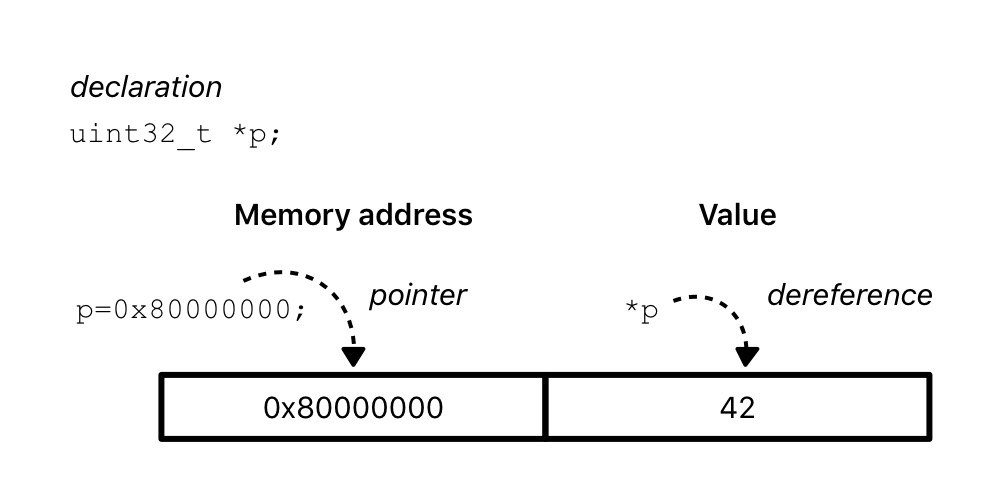
\includegraphics[width=0.6\textwidth]{pointer.jpg}}
\caption{Pointer declaration}
\label{PointerImg}
\end{figure}

Figure \ref{PointerImg} shows a declaration of a variable \textit{p} as a pointer. \textit{p} points to a value of type \textit{uint32\_t}. The pointer is shown to be assigned the memory address 0x80000000. To access the value 42 the variable \textit{p} is dereferenced using \textit{*p}. 

\begin{lstlisting}[language=C,showstringspaces=false,caption={File: swap.c, part 1 swap function},captionpos=b,label=swap]

 1 #include <stdio.h>
 2 #include <assert.h>
 3 #include <stdint.h>
 4 
 5 void swap (uint32_t *a,uint32_t *b)
 6 {
 7 uint32_t tmp;
 8 
 9 assert ((a!=NULL)&&(b!=NULL));
10   if (a==b) return;
11 
12 tmp = *a;
13 *a = *b;
14 *b = tmp;
15 }
 
\end{lstlisting}

Listing \ref{swap} shows the function \textit{swap(...)} function. It takes two pointers of type \textit{uint32\_t} called \textit{*a} and \textit{*b} respectively. The variables are checked to see whether they are non-NULL, see line:9. If either variable is NULL then the program will terminate. Line:10 checks to see if the pointers point to the same memory address. If so then there is no requirement to do the swap. Lines:12-14 carries out the swap mechanism, swapping the values in the locations of \textit{a} and \textit{b} in memory.

\subsection{Reference pointers}
 
\index{pointers!references}
 
A \textit{reference} is symbolized by the character \& i.e.  \&\textless{variable name}\textgreater. A reference variable is fixed to a specific address, it cannot be used in an arithmetic calculation and can only be assigned at initialization time.

\begin{figure}[H]
\centerline{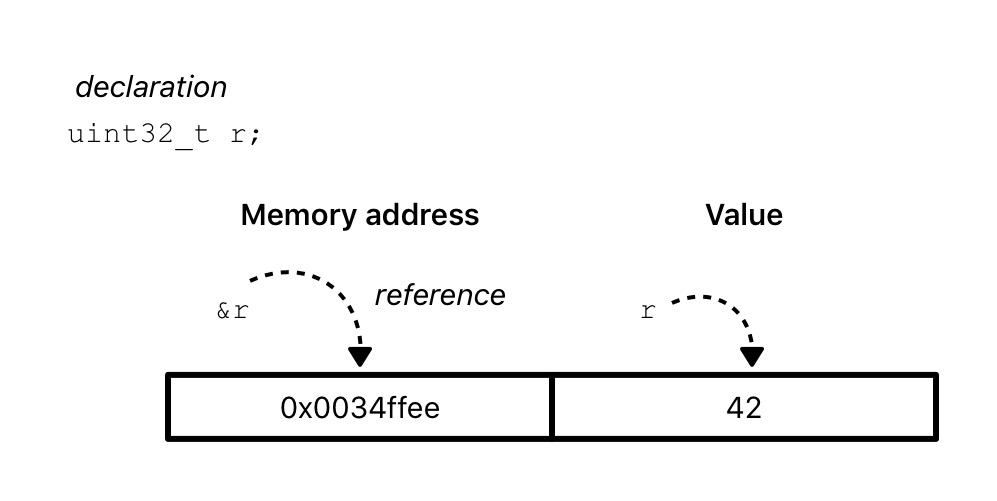
\includegraphics[width=0.6\textwidth]{reference.jpg}}
\caption{Reference declaration}
\label{ReferenceImg}
\end{figure}

Figure \ref{ReferenceImg} shows a declaration of a variable \textit{r} of type \textit{uint32\_t}. To obtain the memory address or reference pointer for \textit{r}, \&\textit{r} is used. In the figure, the reference pointer is memory address 0x0034ffee. To access the value 42 the variable \textit{r} is simply used. This reference pointer is fixed by the compiler at build time. 
   
\begin{lstlisting}[language=C,showstringspaces=false,caption={File: swap.c, part 2},captionpos=b,label=reference]

18 int main(void)
19 {
20 uint32_t x=10,y=20;
21 
22 printf("...start swap\n");
23 printf(" x memory address : 0x%08x\n",(uint32_t)&x);
24 printf(" y memory address : 0x%08x\n",(uint32_t)&y);
25 
26 printf("... init: x=%d,y=%d\n",x,y);
27 
28 swap(&x,&y);
29 printf("... swap: x=%d,y=%d\n",x,y);
30 
31 swap(&x,&y);
32 printf("... swap: x=%d,y=%d\n",x,y);
33 
34 return 0;
35 }

INTERACTION

$ cc swap.c
$ ./a.out
...start swap
 x memory address : 0x5666fba8
 y memory address : 0x5666fba4
... init: x=10,y=20
... swap: x=20,y=10
... swap: x=10,y=20
$
\end{lstlisting}

The listing \ref{reference} shows how references and pointers interact. The example shows a double swap of the variables \textit{x} and \textit{y}. Lines:23:24 prints out the memory address assigned to the variables. The memory addresses never change throughout but the data will change. The variables will have the same value at the start and end of the program. The variables are passed as references into the \textit{swap(...)} function. 

\subsection{void *}

\index{pointers!void pointers}

As discussed in section \ref{voidtype}, \textit{void *} is a generic pointer to any object. It is used to build structures of different types. \textit{void *} does not point to a specific type with a particular size. It is useful for building generic functions that cover multiple different datatypes. 

\subsection{Function pointer}

\index{pointers!function pointer}

The function pointer concept is a powerful feature in the C Programming Language. It allows a function to be a variable. This means that a function can be passed in as a parameter, as well as being placed in a table or structure. We will discuss the table and structure concept in more detail in section \ref{datastructure}.
 
\begin{lstlisting}[language=C,caption={Function Pointer Syntax},captionpos=b,label=functpointer]

<return-type> (*<function pointer name>)({<parameter-list>})

\end{lstlisting}

Listing \ref{functpointer} shows the syntax of a function pointer. The function pointer has a \textit{return-type} similar to a normal function. The brackets ( ... ) along with the *\textless{function pointer name}\textgreater \, identify a function pointer. The \textit{parameter-list} is the same as a standard function definition. 

\begin{lstlisting}[language=C,showstringspaces=false,caption={File: funpointer.c},captionpos=b,label=funpointer]

 1 #include <stdio.h>
 2 #include <math.h>
 3 
 4 double calculate45degrees(double (*funct)(double))
 5 {
 6 return funct(45.0);
 7 }
 8 
 9 int main(void)
10 {
11 printf ("sin(45.0) = %lf\n",calculate45degrees(sin));
12 printf ("cos(45.0) = %lf\n",calculate45degrees(cos));
13 
14 return 0;
15 }

INTERACTION

$ cc funpointer.c
$ ./a.out
sin(45.0) = 0.850904
cos(45.0) = 0.525322
$

\end{lstlisting}


Listing \ref{funpointer} shows an example of a generic function call \textit{calculate45degrees(...)} on lines:4-7. The function has a function pointer parameter called \textit{funct}. In the body of the function the function pointer is called with the value of 45.0. The result of invoking this function is returned to the caller, in this case \textit{main(...)}. 

The caller calls \textit{calculate45degrees(...)} twice with different functions, first the \textit{sin(...)} function and then \textit{cos(...)} function as shown on lines:11:12.


 
 \newpage
\section{Arrays}

Arrays are a fundamental part of the C Language. A one dimensional array is denoted by [...] and subsequently a two dimensional array is denoted by [...][...] and finally a three dimensional array by [...][...][...]. Arrays in C are effectively contiguously allocated memory blocks. 

\subsection{One dimensional arrays}

\begin{figure}[H]
\centerline{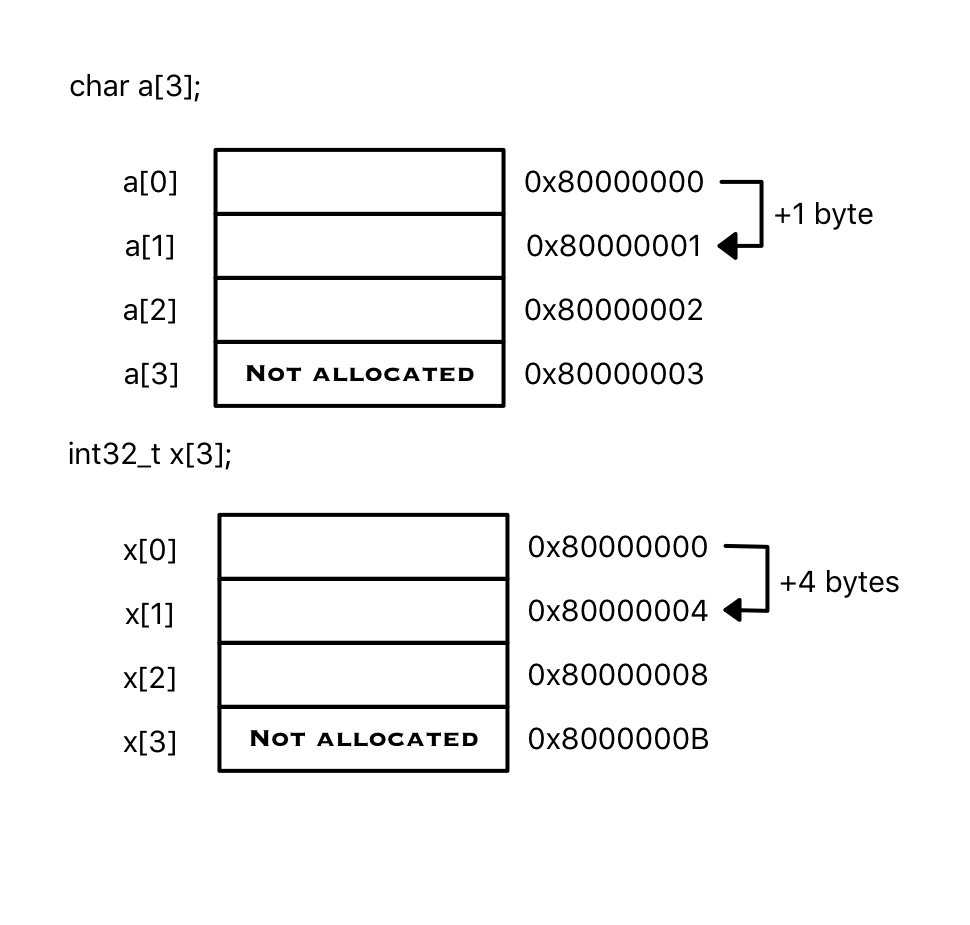
\includegraphics[width=0.6\textwidth]{array.jpg}}
\caption{One dimensional array}
\label{array}
\end{figure}

Figure \ref{array} shows two arrays with the same number of elements but different element sizes. The top array is an array of char's called \textit{a}. Each element of the array is offset by 1 byte taking up a total of four bytes. By comparison, the bottom array is an array of int's. Each element in the array is offset by 4 bytes and is taking up 16 (4x4) bytes. The elements in an \textit{int} array are separated by 4 bytes because i.e. \textit{sizeof(int32\_t)=4}		and for \textit{char}'s by 1 byte i.e. \textit{sizeof(char)=1}.

The sizing of the array looks to be off by one because an array starts at zero, meaning an array declared as \textit{x[4]} does not allocate space for \textit{x[4]} but for \textit{x[0]} to \textit{x[3]}. 

It is also important to realize that C does not check for out-of-bounds issues. This means it is relatively easy to make a mistake and access memory which has not been allocated, potentially causing instability or corruption in the system. The programmer has the responsibility to ensure this doesn't happen.

\begin{lstlisting}[language=C,showstringspaces=false,caption={File: array1d.c, one dimensional array},captionpos=b,label=array1d]

 1 #include <stdio.h>
 2 #include <stdlib.h>
 3 #include <time.h>
 4 
 5 int main (void)
 6 {
 7 char one[10];
 8 unsigned int x;
 9 
10 srand((unsigned int)time(NULL));
11 
12 printf ("\n* one dimensional array \n\n");
13 
14 // set up the one dimensional array
15 
16   for (x=0; x<=9; x++)
17     one[x] = rand() % 10;
18 
19 // printout the one dimensional array
20 
21 printf ("  ");
22   for (x=0; x<=9; x++)  
23     printf (" %d ",x);
24   printf ("\n\n");
25 printf ("0:");  
26   for (x=0; x<=9; x++)  
27     printf (" %d ",one[x]);    
28   printf ("\n\n");
29    
30 return 0;
31 }

INTERACTION

cc array1d.c
$ ./a.out

* 1 * one dimensional array 

   0  1  2  3  4  5  6  7  8  9 

0: 9  0  9  8  4  4  6  3  0  8 

$
\end{lstlisting}

Listing \ref{array1d} shows a one dimensional array of 10 elements i.e. 0 to 9 inclusive. The array \textit{one} is define on line:7. Each element of the array is assigned a random value from 0 to 9, see lines:16:17. Finally the array is printed out on lines:21-28.

\subsection{Two dimensional arrays}

\begin{lstlisting}[language=C,showstringspaces=false,caption={File: array2d.c, two dimensional array},captionpos=b,label=array2d]

 1 #include <stdio.h>
 2 #include <stdlib.h>
 3 #include <time.h>
 4 
 5 int main (void)
 6 {
 7 char two[10][10]; // two dimensional array
 8 unsigned int x,y;
 9 
10 srand((unsigned int)time(NULL));
11 
12 printf ("\n* two dimensional array\n\n");
13 
14 // set up the two dimensional array 
15 
16   for (x=0; x<=9; x++)
17     for (y=0; y<=9; y++)
18       two[x][y] = rand() % 10;
19    
20 // printout the two dimensional array
21 
22 printf ("  ");
23   for (x=0; x<=9; x++)  
24     printf (" %d ",x);
25   printf("\n\n");
26 
27   for (y=0; y<=9; y++)
28   {
29   printf ("%d:",y);
30     for (x=0; x<=9; x++)
31       printf (" %d ",two[x][y]);
32   printf ("\n");
33   }
34 printf ("\n");
35 
36 return 0;
37 }

INTERACTION

$ cc array2d.c
$ ./a.out

* 2 * two dimensional array

   0  1  2  3  4  5  6  7  8  9 

0: 2  8  7  0  1  5  1  8  8  8 
1: 3  3  6  8  3  6  1  1  0  6 
2: 3  7  6  9  8  0  0  0  6  9 
3: 1  4  4  8  5  3  7  3  6  1 
4: 8  8  1  8  2  0  5  0  4  5 
5: 2  4  9  2  8  9  8  5  1  9 
6: 9  6  2  1  1  8  0  5  5  0 
7: 9  3  7  6  1  9  9  9  2  8 
8: 1  4  4  1  2  1  6  3  5  8 
9: 8  7  0  4  5  8  2  9  8  3 

$
\end{lstlisting}


listing \ref{array2d} shows a two dimensional array of 10x10 elements. Line:7 declares the array. Lines:16-18 initializes the 2D array, again with a random number between 0 and 9. Once initialized the array is printed out, as carried out by the code on lines:22-34.

\subsection{Three dimensional arrays}


\begin{lstlisting}[language=C,showstringspaces=false,caption={File: array3d.c, three dimensional array},captionpos=b,label=array3d]

 1 #include <stdio.h>
 2 #include <stdlib.h>
 3 #include <time.h>
 4 
 5 int main (void)
 6 {
 7 char three[10][10][10]; // 3 dimensional array
 8 unsigned int x,y,z;
 9 
10 srand((unsigned int)time(NULL));
11 
12 printf ("\n* three dimensional array \n\n");
13 
14 // set up the three dimensional array
15 
16   for (x=0; x<=9; x++)
17     for (y=0; y<=9; y++)
18       for (z=0; z<=9; z++)
19         three[x][y][z] = rand() % 10;
20 
21 // printout the three dimensional array
22 
23   for (z=0; z<=9; z++)
24   {
25   printf ("\nz:%d\n",z);
26 
27   printf ("  ");
28     for (x=0; x<=9; x++)  
29       printf (" %d ",x);
30     printf("\n\n");
31 
32     for (y=0; y<=9; y++)
33     {
34     printf ("%d:",y);
35       for (x=0; x<=9; x++)
36         printf (" %d ",three[x][y][z]);
37     printf ("\n");
38     }
39   }
40 
41 return 0;
42 }

INTERACTION

$ cc array3d.c
$ ./a.out

* 3 * three dimensional array 

z:0
   0  1  2  3  4  5  6  7  8  9 

0: 6  8  9  8  7  3  1  7  5  8 
1: 2  3  9  7  5  2  8  2  8  7 
2: 9  4  4  6  2  7  8  3  0  3 
3: 9  5  9  8  8  4  8  5  5  6 
4: 1  2  5  4  7  2  4  9  3  1 
5: 2  0  3  9  2  7  7  4  1  2 
6: 4  8  8  2  6  3  1  7  7  9 
7: 2  2  6  6  2  8  9  6  0  7 
8: 1  0  9  0  8  3  5  3  3  3 
9: 2  5  5  8  3  6  7  0  1  8 

...

z:9
   0  1  2  3  4  5  6  7  8  9 

0: 1  5  2  8  5  3  8  7  4  8 
1: 2  6  3  8  3  0  3  2  2  9 
2: 7  3  8  8  0  1  8  0  9  4 
3: 9  7  9  8  0  9  2  5  6  6 
4: 9  4  2  6  5  5  6  7  3  5 
5: 9  3  2  5  8  3  0  5  8  9 
6: 1  1  6  5  0  5  4  1  3  4 
7: 8  5  4  6  7  9  4  7  7  9 
8: 2  7  5  0  6  6  1  4  4  8 
9: 4  9  5  5  0  7  5  9  7  1 

$

\end{lstlisting}

Listing \ref{array3d} shows a three dimensional array with 10x10x10 elements. Similar to listing \ref{array1d} and \ref{array2d} the array is created, initialized and displayed. The real difference being that a three dimensional array is more complicated to printout. 

For optimal performance, it is recommended that the code follow the layout of the target hardware cache. Hardware caches are designed with specific data lengths. The nearer any data format is to these lengths the more efficient and faster the throughput. This can have significant improvements on array manipulation performance since it can take advantage of the temporal and spacial characteristics of the target hardware. 

Particular performance cases may require some extra padded records. Enforcing data alignment with a specific cache architecture i.e. line length, can produce significant performance improvements although at the cost of increasing memory usage. This comes at the cost of increasing memory size. The inverse is to pack structures to maximize memory utilization. This may slow a program down due to the high frequency of cache misses. A general rule for optimal performance is to align data as much as possible with the cache architecture being used.

Arrays are used to create queues, circular buffers, stacks and strings in C.

\subsection{Passing arrays into functions}

Passing arrays into functions can be carried out using a number of different methods, as shown in listing \ref{arraypass}.

\begin{lstlisting}[language=C,showstringspaces=false,caption={File: arraypass.c},captionpos=b,label=arraypass]

 1 #include <stdio.h>
 2 #include <stdint.h>
 3 
 4 
 5 void print_out_1darray(char *a1,uint8_t size)
 6 {
 7   do
 8   {
 9   a1[size] = size;
10   printf("array[%d] = %d\n",size,a1[size]);
11   }
12   while (size--);
13 }
14 
15 void print_out_2darray(char a2[2][2])
16 {
17 uint8_t y=1,x;
18   do
19   {
20   x = 1;
21     do
22     {
23     a2[x][y] = x+y;
24     printf("array[%d,%d] = %d\n",x,y,a2[x][y]);
25     }
26     while (x--);
27   }
28   while (y--); 
29 }
30 
31 void print_out_3darray(char (*a3)[2][2])
32 {
33 uint8_t z=1,y,x;
34   do
35   {
36   y = 1;
37     do
38     {
39     x = 1;
40       do
41       {
42       a3[x][y][z] = x+y+z;
43       printf("array[%d,%d,%d] = %d\n",x,y,z,a3[x][y][z]);
44       }
45       while (x--);
46     }
47     while (y--);
48   }
49   while (z--);
50 }
51    
52 int main(void)
53 {
54 char _a1[2],_a2[2][2],_a3[2][2][2];
55 
56 print_out_1darray(_a1,1);
57 print_out_2darray(_a2);
58 print_out_3darray(_a3);
59 
60 return 0;
61 }

INTERACTION

$ cc arraypass.c
$ ./a.out
array[1] = 1
array[0] = 0
array[1,1] = 2
array[0,1] = 1
array[1,0] = 1
array[0,0] = 0
array[1,1,1] = 3
array[0,1,1] = 2
array[1,0,1] = 2
array[0,0,1] = 1
array[1,1,0] = 2
array[0,1,0] = 1
array[1,0,0] = 1
array[0,0,0] = 0
$
\end{lstlisting}

Listing \ref{arraypass} shows a method to pass a single dimensional array, a two dimensional array and a three dimensional array. The first example, \textit{print\_out\_1darray(...)} shows a one dimensional array being passed in, as shown on lines:5-13. The array is passed as a pointer plus an argument defining the size of the array. 

The second example on lines:15-29 \textit{print\_out\_2darray(...)}, shows a two dimensional array with a fixed size [2][2]. 

Finally the third example on lines:31-50 \textit{print\_out\_3darray(...)}, shows a three dimensional array being passed as a pointer to a fixed two dimensional array [2][2]. Essentially passing an array into a function is basically passing the address of the beginning of the array. 


\newpage
\section{Strings}

\index{string.h}

The C Programming Language doesn't have a specific type dedicated for strings. Instead it makes use of \textit{char arrays} to represent a string. A string is defined as an array of characters (char's) terminated by a char value 0. In other words, a string is simply an one-dimensional array of char's which has an extra element at the end set to 0. 

In this section we will cover three common string functions which are available, but note there are many more string functions available.

\begin{figure}[H]
\centerline{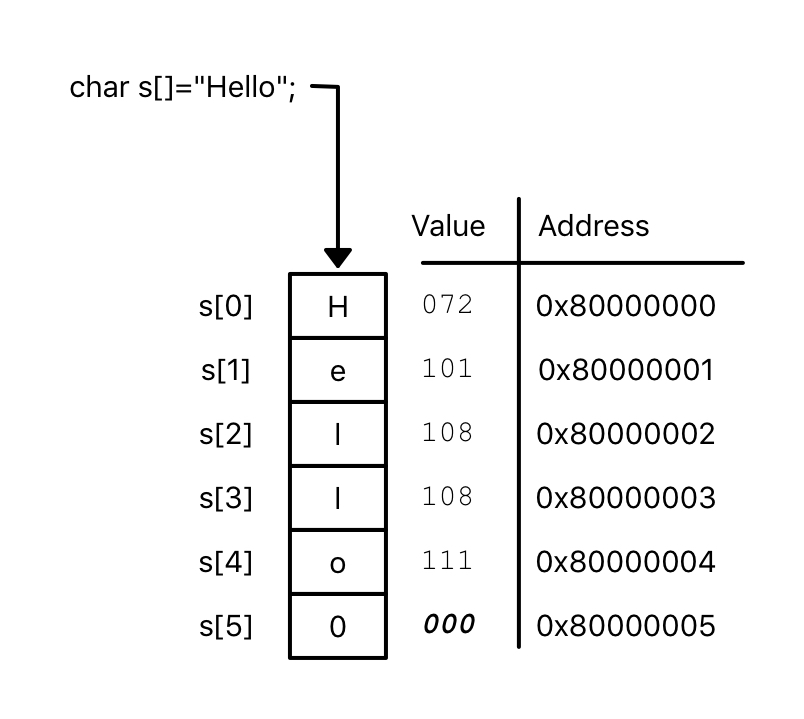
\includegraphics[width=0.6\textwidth]{string.jpg}}
\caption{"Hello" string as a char array}
\label{HelloString}
\end{figure}

The figure \ref{HelloString} shows the "Hello" string represented in memory. The last location in the array s[5] contains 0 which terminates the string. If we calculate the entire length of the string it is 5 ("Hello") + 1 (0, Terminator) which is 6 and not 5.  

\subsection{strlen(...)}

\index{strlen(...)}

The function \textit{strlen(...)} returns the length of a string but unfortunately it returns the length without the 0 terminator. It is important when defining a string to include the 0 terminator within the calculation. The compiler will allocate the right amount of space when compiling but the code itself has to take into account the additional string terminator.

\begin{lstlisting}[language=C,showstringspaces=false,caption={File: strlen.c},label={strcmp},captionpos=b,label=strlen]

 1 #include <stdio.h>
 2 #include <string.h>
 3    
 4 int main(void)
 5 {
 6 char str1[] = "Hello";
 7 
 8 printf("... string length \"Hello\"   = %lu\n",strlen(str1));
 9 printf("... string length \"Hello\"+0 = %lu\n",strlen(str1)+1);
10  
11 return 0;
12 }

INTERACTION

$ cc strlen.c
$ ./a.out
... string length "Hello"   = 5
... string length "Hello"+0 = 6
$

\end{lstlisting}

Listing \ref{strlen} shows the forming of a string and then obtaining the string length. Line:6 shows a string being formed. The array doesn't have a fixed size [], this number is provided by the compiler. Line:8 outputs the \textit{strlen(...)} function which shows that it only provides the length of the string without the terminator. Line:9 adds the 0 terminator to the string length.

\subsection{strcmp(...)}

\index{strcmp(...)}

Similar to many programming languages, string comparisons are treated slightly differently from the general mathematical comparisons i.e. ==. In C a function such as \textit{strcmp(...)} is used to carry out a string comparison. This function can be found in the \textit{string.h} standard library. 

\begin{lstlisting}[language=C,showstringspaces=false,caption={File: strcmp.c},label={strcmp},captionpos=b]

 1 #include <stdio.h>
 2 #include <string.h>
 3 
 4 int main(void)
 5 {
 6 char str1[] = "abcdefg";
 7 char str2[] = "12345";
 8 
 9   if (!strcmp(str1,"abcdefg"))
10     printf("... 1 str1 equal to \"abcdefg\" \n");
11   else
12     printf("... 1 str1 not equal to \"abcdefg\" \n");
13 
14   if (!strcmp(str1,str2))
15     printf("... 2 str1 equal to str2 \n");
16   else
17     printf("... 2 str1 not equal to str2 \n");
18 
19 return 0;
20 }

INTERACTION

$ cc strcmp.c
$ ./a.out
... 1 str1 equal to "abcdefg" 
... 2 str1 not equal to str2 
$

\end{lstlisting}

Listing \ref{strcmp} shows an example of using \textit{strcmp}. The code carries out two comparisons. The first tests to see if \textit{str1} is equal to the fixed string "abcdefg", as shown on line:9. The second test checks whether two string arrays are the same, as shown on line:14. The first should be true and the second should be false.

\subsection{strcpy(...)}

\index{strcpy(...)}

The \textit{strcpy(...)} function copies a source string to a destination string and returns a pointer to the destination string. The important part is that the destination string points to enough memory to contain a copy of the source string. In other words care has to be taken to make sure there is sufficient memory for the copy. If insufficient memory is allocated for the destination string then a program can become corrupt, as data overwrites either variables or code.  

Corruption leads to instability. These errors are difficult to track down, as they tend to emerge in different forms. The C compiler does not provide any assistance in identifying these types of errors. It is the responsibility of the programmer.  

\begin{lstlisting}[language=C,showstringspaces=false,caption={File: strcpy.c},captionpos=b,label=strcpy]

 1 #include <stdio.h>
 2 #include <string.h>
 3   
 4 int main (void)
 5 {
 6 char src[] = "Hello";
 7 char dest[10];
 8   
 9 printf ("dest \"%s\" == src \"%s\"\n",strcpy(dest,src),src);
10 
11 return 0;
12 }

INTERACTION

$ cc strcpy.c
$ ./a.out
dest "Hello" == src "Hello"
$

\end{lstlisting}

Listing \ref{strcpy} shows a string copy. The destination string \textit{dest[10]} has a fixed length of 10 characters and the source string \textit{src[6]} has a fixed length of 6 characters allocated. The \textit{strcpy(...)} function on line:9 returns a pointer to the destination string. This string is then used  by the \textit{printf(...)} to output the result of the function.
  
 

\newpage
\section{Program memory layout} \label{Memory Layout}

This section explores how a C Program is laid out in memory. We will use the GNU C Compiler memory layout as the template. Each operating system and C compiler combination may have slightly different naming conventions but the underlying principles remain the same.
 \begin{figure}[H]
\centerline{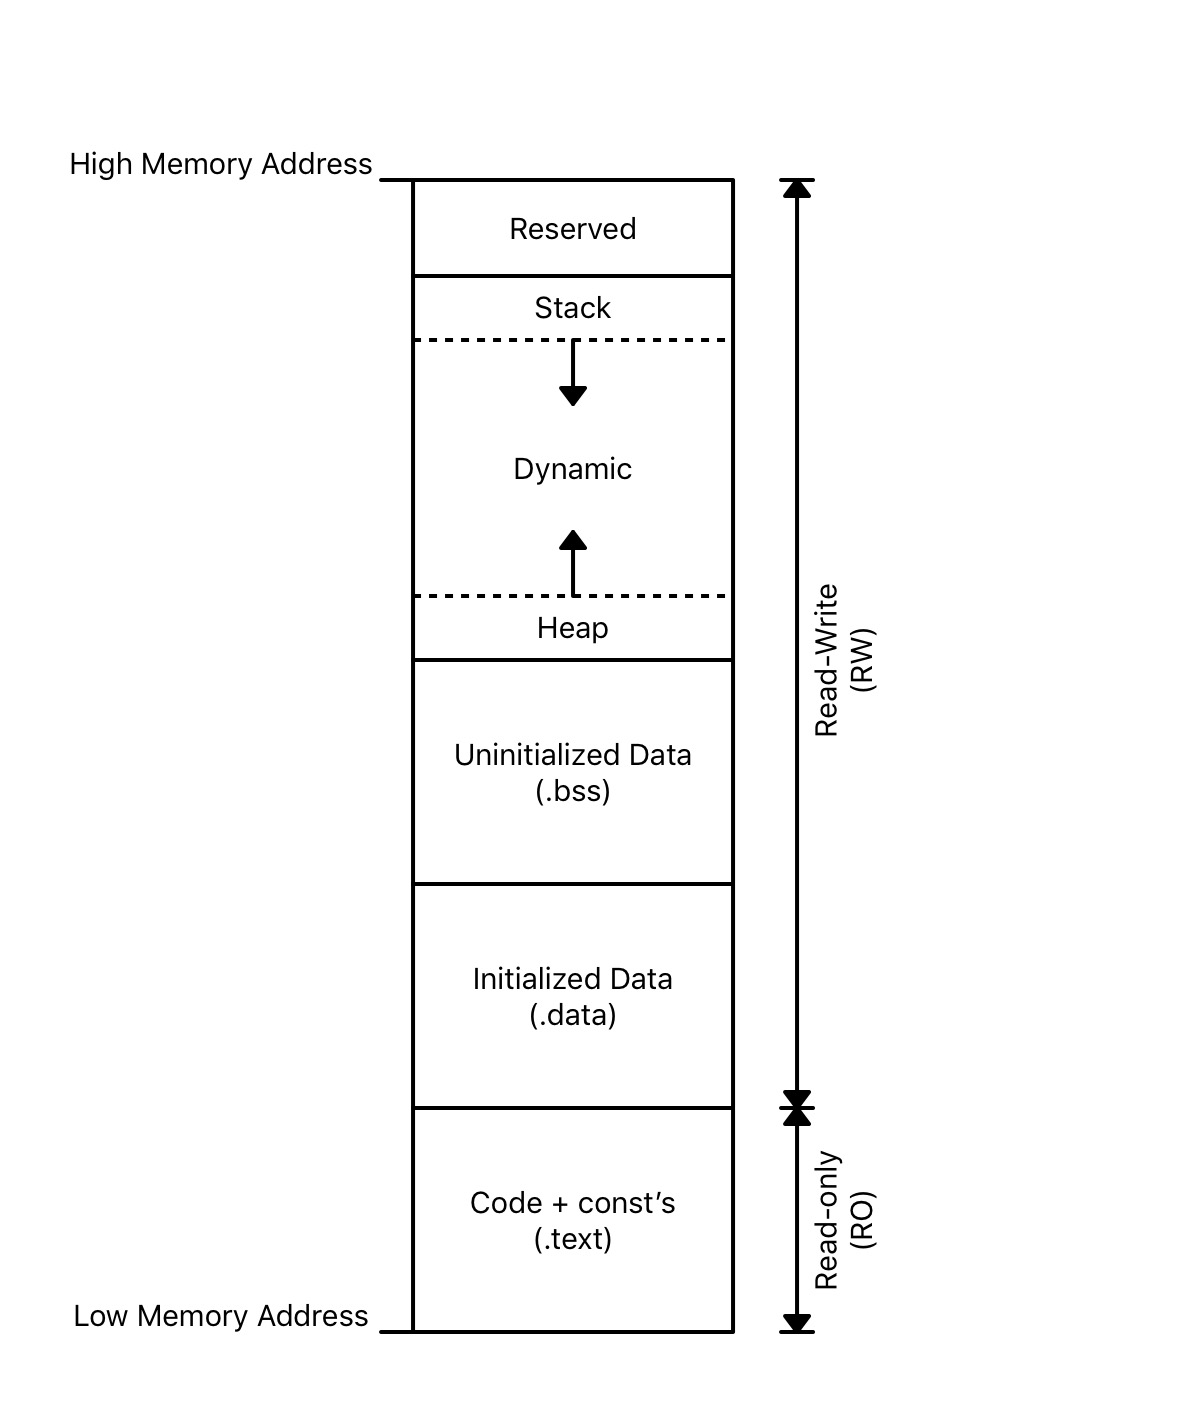
\includegraphics[width=0.6\textwidth]{layout.jpg}}
\caption{C Program Memory Layout}
\label{CProgMem}
\end{figure}

For simplicity we will just explore a single threaded C program, as shown in figure \ref{CProgMem}. A program is divided into a number of memory segments i.e. \textit{.text}, \textit{.data}, \textit{.bss} and finally the \textit{dynamic} and \textit{reserved} areas. For a multi-threaded program there will be a stack dedicated to each thread within the dynamic area. 

When compiling and linking for an embedded system it is important control where individual segments are physically located. For some systems the segments may not be contiguous and in fact may be purposely placed in specific memory types. These types may have different read-write attributes, size capacity, longevity or even power characteristics.    

Note, figure \ref{CProgMem} has low memory addresses at the bottom ascending to higher memory addresses at the top. For a reminder about variable types recommend going back to section \ref{avari}.

\newpage

\begin{lstlisting}[language=C,showstringspaces=false,caption={Image segment breakdown},captionpos=b,label=filesize]
 1 $ size calling.o
 2  text	   data	    bss	    dec	    hex	filename
 3   196	      0	      0	    196	     c4	calling.o
 4 $ 
\end{lstlisting}

Listing \ref{filesize} shows the breakdown of a object file \textit{calling.o}. The listing shows that the object only contains instruction code (text) and no initialized (data) nor uninitialized (bss) data. This information is extracted using the GNU compiler utility tool \textit{size}. 

\subsection{.text segment} \index{.text}

\textit{.text} memory segment is a fixed size non-modified memory area that contains the executable instructions (and the \textit{const} variables) of a C program. The size is determined by the compiled source code. It is a read-only segment since neither the instructions nor the \textit{const} variables should be modified during the lifetime of the program. 

The read-only attribute means that this segment can be placed (and executed) in nonvolatile memory. This can be important when dealing with embedded systems. Especially if the volatile memory is limited in size.

\subsection{.data segment} \label{.data} \index{.data}

\textit{.data} memory segment is a fixed size and contains the initialized data (e.g. \textit{x=42;}). The data represents global or static variables which have been set a value and can be modified. The number of variables determines the size of the segment. For deeply embedded systems it is common for the \textit{.data} segment to first reside in non-volatile memory. During the program startup initiation the \textit{.data} segment is copied from non-volatile memory to some form of volatile memory. The volatile memory allows the data to be modified during program execution.

\subsection{.bss segment} \index{.bss}

\textit{.bss} memory segment is a fixed size and contains uninitialized data. The data is a combination of global and static variables which are not initialized to a specific value by the program (e.g. \textit{static int x;}). The number of variables determines the size of the segment. For this reason variables are initially set to the value zero. This is normally achieved programmatically using a loop to set the variables to zero.

Similar to \textit{.data} segment, in section \ref{.data}, the \textit{.bss} segment is held in volatile memory because these variables may change in value as the program executes.

\subsection{Dynamic area}

Dynamic segment is the part of the memory layout that grows and shrinks depending upon usage. The size limit remains constant. Contrary to \textit{.text}, \textit{.data} and \textit{.bss} segments which remain fixed size throughout the lifetime of the program. The dynamic segment contains both the \textit{C User Stack} and the \textit{Heap} which are continuously growing and shrinking during program execution.

\subsubsection{Program stack}

The program stack is used during calculations, preserving data, restoring data and calling functions. Each hardware architecture has a unique way to call functions and return values. This is normally standardized in a document called the \textit{Procedure Call Standard} (PCS), explained in more detail in section \ref{callingass}. The PCS defines how parameters are passed into a function and how the return values are stored. For many architectures the first n-parameters are passed in as registers and all subsequent parameters are held on the stack. These parameters are held on program stack. Also the function return address can also be held on the stack.  

\subsubsection{Heap}

The \textit{heap} is the area where dynamic memory is stored and removed. It competes with the same for memory as the stack. For more details on \textit{Dynamic Memory Allocation} see section \ref{DynamicMem}.

For embedded systems the heap may be used during the initialization phase but after that point the heap will remain fixed in size i.e. it neither grows nor shrinks. This is because dynamic memory is difficult in control in systems where high reliability is required.

\subsection{Reserved area}

This area of memory is reserved for command line inputs and environment details when the C program is called.
  
\newpage
\section{Dynamic Memory Allocation} \label{DynamicMem}

Dynamic memory is the allocation and deallocation of memory while a program is executing. It is used primarily for building data structures where the amount of memory required is unknown. There are two main mechanisms, the first is to allocate memory and the second is to deallocate memory. The C programming language offers two main functions, namely \textit{malloc(...)} and \textit{free(...)}. There are many variations but we will concentrate on these two specific functions.  

Once memory has been allocated there are number of useful functions that are available to initialize and copy memory. These functions are \textit{memset(...)} and \textit{memcpy(...)}.  

A \textit{memory leak} is when memory that is no-longer required remains allocated and forgotten. If this problem remains unchecked and continues to grow in severity, then the program will finally halt due to a lack of available memory. Memory leaks can be a major cause of program failure.
 
For deeply embedded or safety-critical systems, dynamic memory is not recommended for general use. During the initialization phase it is acceptable to use dynamic memory to create the right environment but once executing the memory is recommended to be treated as static or non-dynamic. Even in this case, it is quite common to implement an allocator which will look somewhat like a memory pool (fixed-block size allocation).

\subsection{malloc(...)}

\index{malloc(...)}

The \textit{malloc(...)} function dynamically allocates memory in the system. This memory is allocated in a place called the \textit{heap}. The \textit{heap} is an area of memory dedicated to dynamic memory. Once memory has been successfully allocated a starting address is returned. If the memory allocation is unsuccessful NULL is returned.

\begin{lstlisting}[language=C,showstringspaces=false,caption={File: malloc.c},captionpos=b,label=malloc]

 1 #include <stdio.h>
 2 #include <stdlib.h>
 3 #include <string.h>
 4 
 5 int main(void)
 6 {
 7 char src[]="Hello";
 8 char *dest;
 9 
10 dest = (char *)malloc(strlen(src)+1);
11 
12   if (dest==NULL)
13   {
14   fprintf(stderr,"error: malloc failed to allocate in %s at %d\n",__FILE__,__LINE__);
15   exit(EXIT_FAILURE);
16   }
17 
18 printf ("dest \"%s\" == src \"%s\"\n",strcpy(dest,src),src);
19  
20 return 0;
21 } 

INTERACTION

$ cc malloc.c
$ ./a.out
dest "Hello" == src "Hello"
$

\end{lstlisting}

Listing \ref{malloc} shows code that allocates 100 integers, each integer takes up 4 bytes which effective means 400 bytes are allocated or reserved. The allocation occurs on line:18. The sizeof macro calculates the size of a specific type, in this case it returns the value 4. \textit{malloc(...)} allocates bytes.

There are a number of variations of this function and it may be worth exploring further what those variations provide. 

For embedded programmers, there is often a requirement to allocate a large amount of memory. This is achieved using arrays. The arrays are statically defined at the beginning of the program or system. When smaller memory chunks are required they are taken from the free spaces in the arrays. All the allocation management is controlled by the programmer directly.

\subsection{free(...)}

\index{free(...)}

The C Programming Language, unlike some other languages which automatically free unused memory i.e. garbage collection, does not deallocate memory automatically. This job is left to the programmer. It is always good policy to deallocate dynamic memory which is no longer required or before a program terminates. 

Memory deallocation is achieved using the \textit{free(...)} function. It releases an important resource which can be used by another program or even the same executing program. This method of deallocating memory is relatively simple and is achieved by passing the pointer, provided by \textit{malloc(...)}, into the \textit{free(...)} function. The memory is then no longer protected.

When a User program (process) terminates either unexpectedly or planned, the process is destroyed. This means all the associated allocated memory for that specific process is deallocated and free-ed. For an operating system kernel or device driver there may be more complicated scenarios to handle. It is good practice to deallocate all allocated memory when exiting a kernel function or device driver when that memory is no-longer required. In other words, don't assume the system will take care of allocated memory no-longer in-use.    

\begin{lstlisting}[language=C,showstringspaces=false,caption={File: free.c},captionpos=b,label=free]

 1 #include <stdio.h>
 2 #include <stdint.h>
 3 #include <stdlib.h>
 4 
 5 int main(void)
 6 {
 7 uint8_t *ptr;
 8 
 9 ptr = (uint8_t *) malloc(100*4); // allocate 400 bytes
10   
11   if (ptr==NULL)
12   {
13   fprintf(stderr,"malloc failed %s at %d\n",__FILE__,__LINE__);
14   exit(EXIT_FAILURE);
15   }
16   
17 printf("... successfully allocated 400 bytes, now available \n");
18 
19 /* ... do something useful */
20 
21 free(ptr); // deallocate 400 bytes
22 
23 printf("... successfully deallocated 400 bytes, now not available \n");
24 
25 return 0;
26 }

INTERACTION

$ cc free.c
$ ./a.out
... successfully allocated 400 bytes, now available 
... successfully deallocated 400 bytes, now not available 
$ 

\end{lstlisting}

Listing \ref{free} shows the use of \textit{malloc(...)} and \textit{free(...)}. The example shows the allocation of 400 bytes on line:9 and then the deallocation on line:21. Also notice the casting to a specific type on line:9. If the allocation isn't successful the program terminates. If successful then \textit{free(...)} is called to deallocate the memory.
 
\subsection{memset(...)}
\index{memset(...)}

The \textit{memset(...)} function is used to initialize memory regions. This function can be highly optimized "tuned" for a particular architecture. Tuning involves optimizing to the the target cache architecture of the platform. Performance can vary depending upon whether the data being manipulated is a multiple of the cache line length. This is true for all of the inbuilt memory functions. 

However, please note application portability is sometimes required and more generic memory function implementations are used. This is because the highly optimized versions will not be optimal for all architectures and in some cases will cause fatal errors.

\begin{lstlisting}[language=C,showstringspaces=false,caption={File: memset.c},captionpos=b,label=memset]

 1 #include <stdio.h>
 2 #include <stdlib.h>
 3 #include <stdint.h>
 4 #include <string.h>
 5 #include <time.h>
 6 
 7 int main(void)
 8 {
 9 uint8_t *ptr;
10 int x;
11 clock_t start;
12 
13 ptr = malloc(1024*1024);
14 
15   if (ptr==NULL)
16   {
17   fprintf(stderr,"could not allocate memory");
18   exit(EXIT_FAILURE);
19   }
20 
21 start = clock();
22 memset(ptr,0,(1024*1024)); //zero initialize memory
23 printf ("... time taken to zero 1MB: %lf\n",(double)(clock()-start)/CLOCKS_PER_SEC);
24 
25 free(ptr);
26 
27 return 0;
28 }

INTERACTION

$ cc memset.c
$ ./a.out
... time taken to zero 1MB: 0.000754
$ 
	
\end{lstlisting}

Listing \ref{memset} shows an example of setting memory. The function \textit{memset(...)}, on line:22, sets 1MB of memory to zero. This is a common technique for initializing new memory. Memory can have arbitrary values so by setting it to a known value the memory becomes consistent and if the memory is then used as a pointer without initialization, asserts checking for void will be triggered.

\subsection{memcpy(...)}
\index{memcpy(...)}

\textit{memcpy(...)} does as the name implies, it copies memory from one location to another. Again similar to \textit{memset(...)} there can be highly optimized versions available which are specific to a particular hardware implementation. The optimization levels can vary depending on the size of data being copied. Note for memory regions which overlap it is recommended that \textit{memmove(...)} is used as an alternative. 
\index{memmove(...)}

\begin{lstlisting}[language=C,showstringspaces=false,caption={File: memcpy.c},captionpos=b,label=memcpy]

 1 #include <stdio.h>
 2 #include <stdlib.h>
 3 #include <stdint.h>
 4 #include <string.h>
 5 #include <time.h>
 6 
 7 #define CMAX (1024*1024)
 8 
 9 int main(void)
10 {
11 uint8_t *dest,*src;
12 int x;
13 clock_t start;
14 
15 dest = malloc(CMAX);
16 src = malloc(CMAX);
17 
18   if (dest==NULL || src==NULL)
19   {
20   fprintf(stderr,"could not allocate memory");
21   exit(EXIT_FAILURE);
22   }
23 
24 memset(src,'a',CMAX);
25 
26 start = clock();
27 memcpy(dest,src,CMAX); 
28 printf("- time taken to zero %dB: %lf\n",CMAX,(double)(clock()-start)/CLOCKS_PER_SEC);
29 
30 x=0;
31 
32   while (*(src+x)==*(dest+x) && ++x<CMAX);
33   
34   if (x!=CMAX)
35     printf ("... memcpy failed at %x\n",x);
36 
37 free(src);
38 free(dest);
39 
40 return 0;
41 }

INTERACTION

$ cc memcpy.c
$ ./a.out
- time taken to zero 1KB: 0.000007
$ 

\end{lstlisting}

Listing \ref{memcpy} shows an example using memory copy.  The example simply copies memory from one to location to another. It takes source and destination pointers and the size of the data being copied. The function on line:27 copies CMAX bytes from the \textit{src} location to a \textit{dest} location. Finally the memory locations are compared on lines:32-35. If the memory is inconsistent a message is sent to the console.







 
\newpage
\section{Accessing assembly code from C} \label{assembler} \index{assembler}

For embedded systems it is important to access the lowest possible levels of the hardware. These low-level features are hardware specific and not always supported by the programming languages available. To achieve this capability the native assembly language is used. C has two methods of accessing assembly code. The first method involves integrating assembly instructions directly into C source code using an inline assembler (see section \ref{inlineass}) and the second method is by calling assembly routines directly (see section \ref{callingass}). 

These interfaces also allow access to more advanced features of a processor. For example, access to \textit{Single Instruction Multiple Data} (SIMD) instructions for multimedia or fast matrices operations.

Accessing assembly code is architecture and compiler specific. We will provide examples which show accessing the ARMv7-A Instructions Set Architecture (ISA) using the GNU C Compiler. The calling convention for each architecture is unique and is often described in a specification called the \textit{Procedure Call Standard}. Even-though architectures differs in convention the underlying principles remain the same. 


\subsection{Example: ARM Procedure Call Standard} \label{apcs}

This is the calling convention for ARMv7-A ISA. This is used by the GNU C Compiler to call functions on compatible hardware. If you are writing assembly code which is called by C then you have to adhere to the calling convention, non-adherence can potentially result in unpredictable behavior. The information in this section was taken from \textit{Procedure Call Standard for the ARM Architecture, ARM IHI 0042F, current through ABI release 2.10}. Note, ABI stands for Application Binary Interface. 

\begin{table*}[ht]
\centering
  \begin{tabular}{ | c | c | l |}
    \hline
    REG & NAME & DESCRIPTION \\ \hline
    r0  & a1   & parameter, result or scratch  \\ \hline
    r1  & a2   & parameter, result, or scratch  \\ \hline
    r2  & a3   & parameter or scratch \\ \hline
    r3  & a4   & parameter or scratch \\ \hline  
    r4  & v1   & variable  \\ \hline
    r5  & v2   & variable  \\ \hline
    r6  & v3   & variable  \\ \hline  
    r7  & v4   & variable  \\ \hline
    r8  & v5   & variable  \\ \hline
    r9  & v6, SB or TR & platform variable   \\ \hline  
    r10 & v7   & variable   \\ \hline
    r11 & v8  & variable  \\ \hline  
    r12 & IP  & Intra-Procedure-call scratch register  \\ \hline
    r13 & SP  & Stack Pointer \\ \hline
    r14 & LR  & Link Register \\ \hline 
    r15 & PC  & Program Counter\\ \hline  
  \end{tabular}
\caption{Register allocation}
\label{table:pcs}
\end{table*}

Table \ref{table:pcs} show the declaration that the first four registers \textit{r0-3} are parameter passing registers. These register are used to place data into a function. They are also scratch registers meaning they can be used to hold intermediate values without any worry of corrupting the caller function. Register \textit{r0} and \textit{r1} carry the return result. It is common that only register \textit{r0} hold the return value. 
 
Registers \textit{r4-8} and \textit{r10-11} are used as standard variable registers (note: r9 is special). If a function uses these registers then the registers need to be preserved and restored upon return. The caller function will assume these values are retained before and after invoking the callee function. 

Register \textit{r12} (IP) and in some cases r9, are special cases which are compiler dependent. Check your compiler documentation for details. 

The remaining registers \textit{r13-15} have designated architectural functions. Register \textit{r13} is the stack pointer (for calculations, preserving+restoring context and passing arguments). Register \textit{r14} is the link register which is used to hold the return address within the caller function. And finally \textit{r15} is the program counter, it points to the instruction next to be loaded into the processor. Note registers \textit{r13} and \textit{r14} can be used for general purposes (if and only if restored correctly upon exit).

\subsection{Inline assembly} \label{inlineass} \index{inline assembler}

Inline assembly allows assembler instructions to be inserted directly into C source code. It makes the C code hardware specific. This is useful when short assembly sequences are required to access a specific hardware features or provide some unique optimized instruction flow. It is important that the rules of the compiler are obeyed since the instructions are being embedded in the C routines.

\begin{lstlisting}[language=bash,showstringspaces=false,caption={File: inline.c},captionpos=b,label=inlineassembler]

 1 #include <stdio.h>
 2 #include <stdint.h>
 3 
 4 int main(void)
 5 {
 6 int32_t d = 12345;
 7 int32_t s1 = 10;
 8 int32_t s2 = 20;
 9 
10 __asm("add %[des],%[src1],%[src2]":[des]"=r"(d):[src1]"r"(s1),[src2]"r"(s2));
11   
12 printf("add  %d = %d + %d\n",d,s1,s2);
13 
14 return 0;
15 }

INTERACTION

16 $ cc inline.c
17 $ ./a.out
18 add  30 = 10 + 20
19 $

\end{lstlisting}

Listing \ref{inlineassembler} line:10 shows an \textit{add} instruction inserted into the source code using the keyword \textit{\_\_asm(...)}. The instruction adds two variables \textit{s1} and \textit{s1} together and places the destination result into a variable called \textit{d}.
	
\subsection{Calling assembly routines} \label{callingass}

Calling assembly code is similar to calling any C function. Each architecture has a set of rules to call a function. These rules are layout by the Procedure Calling Standard, defined in section \ref{apcs}. By adhering to the rules an assembly routine can be called from C without causing issues with program. The example set out below shows a small subset of the calling convention. 

\begin{lstlisting}[language=bash,showstringspaces=false,caption={File: calling.c},captionpos=b,label=calling]
 1 #include <stdio.h>
 2 #include <stdint.h>
 3 
 4 extern uint32_t _sumof4numbers
 5 (
 6  uint32_t a,
 7  uint32_t b,
 8  uint32_t c,
 9  uint32_t d
10 );
11 
12 extern uint32_t _sumof5numbers 
13 (
14   uint32_t a,
15   uint32_t b,
16   uint32_t c,
17   uint32_t d,
18   uint32_t e
19 );
20 
21 extern uint32_t _example_42(void);
22 
23 int main (void)
24 {
25 uint32_t s4,s5,d42;
26 
27 s4 = _sumof4numbers (1,2,3,4);
28 s5 = _sumof5numbers (1,2,3,4,5);
29 d42 = _example_42();
30 
31 printf ("Procedure Call Standard \n");
32 printf ("-- sum(1,2,3,4)   =  %d\n",s4);
33 printf ("-- sum(1,2,3,4,5) =  %d\n",s5);
34 printf ("-- 42 == %d : %d\n",d42,42==d42);
35 
36 return 0;
37 }
\end{lstlisting}

Listing \ref{calling} shows code which calls three assembly routines, namely \textit{\_sumof4numbers(...)}, \textit{\_sumof5numbers(...)} and \textit{\_example\_42(...)}. These routines represent different ways assembly functions can be called in C. These routines are defined as being \textit{extern's} on lines:4-21. The results of all three routines is then printed out.

The first example \textit{\_sumof4numbers(...)} shows four arguments being passed into a function. The four arguments all fit into the parameter passing registers r0-3. These are defined as the parameter passing registers and scratch registers. Scratch means that they do not require preserving during the call.

The second example \textit{\_sumof5numbers(...)} shows five parameters being passed, the first four fit into the standard registers, the fifth parameter is placed on the stack automatically by the compiler. 

Finally the third example \textit{\_example\_42(...)} defines a function with no parameters being passed into a function.

\begin{lstlisting}[language=bash,showstringspaces=false,caption={File: arm.s},captionpos=b,label=arms]
 1      .text
 2      .global _sumof4numbers
 3      .global _sumof5numbers
 4      .global _example_42
 5 
 6 _sumof4numbers:
 7      add     r0,r0,r1
 8      add     r0,r0,r2
 9      add     r0,r0,r3
10      add     r0,r0,r4
11      bx      lr
12 
13 _sumof5numbers:
14      add     r0,r0,r1
15      add     r0,r0,r2
16      add     r0,r0,r3
17      add     r0,r0,r4
18      ldmia   sp!,{r2}
19      add     r0,r0,r2 
20      bx      lr
21 
22 _example_42:
23     push    {r4-r6,r14}  // prologue - preserve
24     mov     r4,#40
25     mov     r5,#2
26     add     r0,r4,r5
27     pop     {r4-r6,r15}  // epilogue - restore
28 
29     .end

INTERACTION

30 $ cc calling.c arm.s
31 $ ./a.out
32 Procedure Call Standard 
33 -- sum(1,2,3,4)   =  10
34 -- sum(1,2,3,4,5) =  15
35 -- 42 == 42 : 1
36 $
 
\end{lstlisting}

Listing \ref{arms} are the assembly implementations of the functions defined in listing \ref{calling}. The .text on line 1 indicates to the compiler that the information below are instructions. The .global identifies the function names to be exported and used by the linker. In this case \textit{\_sumof4numbers}, \textit{\_sumof5numbers} and \textit{\_example\_42} are all globally exported.

Function \textit{\_sumof4numbers} sums four numbers passed into the routine by registers \textit{r0-3}. The result is left in register \textit{r0} and the routine returns using the instruction on line 20. The link register \textit{lr} (\textit{r14}) holds the return address of where the routine was called by the caller routine. No preserving or restoring of registers is required since all the registered effected were \textit{r0} to \textit{r3}.

Function \textit{\_sumof5numbers} sums five numbers and returns the result. The first four arguments are passed into the routine the same way as \textit{\_sumof4numbers} but the fifth is passed on the stack by the compiler. This value is retrieved by the instruction on line:18. Where it pop's the stack with one register and placed the content into register \textit{r2}. Then adds that value to the sum, creating a sum of five numbers. The rest is same as the previous routine.

Finally function \textit{\_example\_42}, this function takes no parameters but uses two of the variable registers \textit{r4} and \textit{r5}. To make the function compliant with the PCS, these values need to be preserved. This is achieved using the \textit{push} instruction on line:23 which pushes registers \textit{r4-6} onto the stack (\textit{r13}). It also pushes the return address (link register \textit{r14}). A calculation then occurs on lines:24-26, and the result placed into register \textit{r0}. The restore occurs on line:27, where the previously preserved registers \textit{r4-6} are restored along with the link register. The link register contents is placed directly in the program counter which returns execution to the right location in the caller function.  


 
\newpage
\section{Accessing Hardware} \label{Hardware}

C plays an important role when it comes to directly accessing hardware. C code is used to write and read hardware via what is called \textit{memory-mapped registers} \index{memory-mapped registers}. Registers are used to provide multiple functions including status, control and data i/o. A hardware register effectively acts as a contract between the hardware and software. Contracts can be complex and unforgiving, where mistakes or misunderstandings can lead to undesirable consequences. In extreme circumstances these consequences can lead to severe damage or instability of the system. 

 Outside of the processor, memory-mapped registers are similar to memory locations. They are used for everything from initializing external pins to interacting with hardware peripherals (e.g. serial port). Within the processor there are different methods to access registers, each processor architecture is unique in how this is accomplished. We will not discuss how processor registers are accessed since this is architecture specific. 
 
 Externally, memory-mapped registers are assigned memory addresses and depending upon the register-type they allow reading from a register and/or writing to a register. These memory addresses are placed in what is called the \textit{memory-map}. Hardware registers are configured in many different ways, for example a register can be set up to be read-only, write-only or allow both read-write. \index{memory-map}
 
 There can be timing and ordering aspects to registers, an update may not occur instantaneously or one register may not be accessed before another. A register may have bits which remain fixed and cannot or should not be changed. Registers can be private and not available for normal use. 
 
There are many variations and subtleties to consider when accessing hardware registers. Detailed reading of the hardware specification is unavoidable and mandatory at this level. Interfacing with hardware is the ultimate level of control, everything else relies on this low-level engagement being successful.

\subsection{Masks} \index{mask}

Masks are used to guarantee that only specific bits are updated. This is particularly useful when handling memory-mapped registers where each bit can be assigned a special function. The mask is used in conjunction with a \textit{read-modify-write} procedure to read and update a memory-mapped register. \index{read-modify-write}

\begin{enumerate}
\item Read: involves reading a memory-mapped register and placing the value into a variable.
\item Modify: involves two stages. The first involves preparing the data to be updated by forcing the bits for modification to be zero (0). Then the second stage involves updating the bits with new values.
\item Write: finally the new updated variable is written back to the memory-mapped register. 

\end{enumerate}

Modify stage involves first using a \textit{bitwise AND} operation to set the bits for modification to zero. The \textit{mask} bit pattern determines the bits that remain unchanged (i.e. bits set to 1) and the bits to be modified (i.e. bits set 0). The second part involves updating the specific bits by applying a \textit{bitwise OR} operation on the variable with new update bit values. Once the new register value is complete it is then written back to the memory-mapped register.

Note: a \textit{mask} bit pattern means bits set to 1 represent no change and bits set to 0 represent future change. By contrast, \textit{bitwise NOT} \textit{\char`\~mask} bit patterns means the opposite, bits set to 1 represents future change and bits set to 0 are unchanged.

\begin{lstlisting}[language=bash,showstringspaces=false,caption={File: mask.c},captionpos=b,label=mask]

 1 #include <stdio.h>
 2 #include <stdint.h>
 3 
 4 int main(void)
 5 {
 6 uint32_t reg;
 7 uint32_t mask;
 8 
 9 // init values ...
10 reg =  0x12345678; // 0b0001.0010.0011.0100.0101.0110.0111.1000
11 mask = 0xFFF00FFF; // 0b1111.1111.1111.0000.0000.1111.1111.1111
12 
13 printf ("set reg          : 0x%8x \n",reg);
14 printf ("set mask         : 0x%8x \n",mask);
15 
16 // action ...
17 reg &= mask;       // 0b0001.0010.0011.0000.0000.0110.0111.1000
18 
19 printf ("set reg &=  mask : 0x%8x \n",reg);
20 
21 reg |= (0x00054000 & ~mask); // 0b0001.0010.0011.0101.0100.0110.0111.1000
22 
23 printf ("set reg |= new   : 0x%8x \n",reg);
24 
25 return 0;
26 }

INTERACTION

$ cc mask.c
$ ./a.out
set reg          : 0x12345678 
set mask         : 0xfff00fff 
set reg &=  mask : 0x12300678 
set reg |= new   : 0x12354678 
$

\end{lstlisting}

Listing \ref{mask} shows a simple example of using a mask with a binary pattern. On line:11 a mask is set to 0xFFF00FFF. This bit mask sets bits 0-11 and 20-31 to one (1), and bits 12-19 to zero (0). Line:17 shows the \textit{mask} being applied to \textit{reg}, using a \textit{bitwise AND} operation. All the values from bits 0-11 and 20-31 remain unchanged (i.e. where ever a bit is 1 in the \textit{mask}) after the operation, whereas the middle bits 12-19 are forced to be zero (0) i.e. = 0b000100100011\textbf{00000000}011001111000. 

Line:21 shows only bits 12-19 being updated in the \textit{reg} variable, the rest of the bits remain unchanged. This example doesn't use a real hardware register but shows the procedure of setting specific bits within a 32-bit unsigned integer variable. The final result is the 45 is replaced with 54 in the middle of the final value i.e. 0x123\textbf{54}678.  .

\subsection{Define's and data structures}

There are effectively two standard methods to access hardware registers within C. The first uses the \textit{\#define} macro. This method is portable and straightforward, as-in it doesn't require much in the way of compiler support. The second is more elegant and uses bitfield structures to map hardware registers. The structures can be less portable and slightly more complicated to get right. Both methods have advantages and disadvantages.

\subsubsection{Using define's}

This method simply accesses the hardware registers using absolute memory addresses. It is quite obvious that the code is dealing with hardware memory addresses since the addresses are handled by \textit{\#define}'s. The main disadvantage it that is is quite detailed and requires a lot of bitwise manipulations.

\begin{lstlisting}[language=bash,showstringspaces=false,caption={File: volhwreg.c},captionpos=b,label=rawaccess]
	
 1 #include <stdio.h>
 2 #include <stdint.h>
 3 
 4 #define REG_COMMS      0x80000000
 5 #define VOLATILE8(s)   *(volatile uint8_t *)(s)
 6 
 7 int main(void)
 8 {    
 9 uint8_t comms;
10 
11 // READ ...
12 comms = VOLATILE8(REG_COMMS); 
13 
14 // MODIFY ...
15 comms &= 0x80; /* bitwise AND 0b_000.0000 = 00  */
16 comms |= 0x22; /* bitwise OR  0b_010.0010 = 34  */ 
17 comms |= 0x80; /* bitwise OR  0b1010.0010 = 180 */
18 
19 // WRITE ...
20 VOLATILE8(REG_COMMS) = comms;
21 
22 // OUTPUT
23 printf ("parity: %d\n",(VOLATILE8(REG_COMMS) & 0x80) >> 7);
24 printf ("data: %d\n",(VOLATILE8(REG_COMMS) & 0x7F));
25 
26 return 0;
27 }

\end{lstlisting}

Listing \ref{rawaccess} shows a fictitious peripheral called COMMS. The COMMS peripheral register  is located at address 0x80000000, shown on lines:4:5. Line:4 shows a simple \textit{\#define} defining a macro called \textit{REG\_COMMS} to be set at an address 0x80000000. By contrast, line:5 casts a value to a volatile 8-bit unsigned int pointer. This useful when either reading or writing to a hardware register.

Line:12 reads an unsigned 8-bit value from the \textit{REG\_COMMS} peripheral. Lines:15-17 modify the value. In this example line:15 clears the \textit{comms} value from bit 0 to 6 with a \textit{bitwise AND} operation. Bit 7 is left alone as the the parity bit until line:17 where it is set to 1 with a \textit{bitwise OR} operation. Finally line:20 writes the result back to the hardware register.

\subsubsection{Using bitfields} \index{bitfields}

Bitfields are a method of using a data structure to define the fields within a hardware register. It is a more elegant way to access hardware registers since access via a data structure rather than macros containing memory addresses. Each bitfield is labelled and accessed independently.  

\begin{lstlisting}[language=bash,showstringspaces=false,caption={File: bitfield.c},captionpos=b,label=bitfield]

 1 #include <stdio.h>
 2 #include <stdint.h>
 3 
 4 typedef struct
 5 {
 6 uint8_t /* RW */ data:7;
 7 uint8_t /* RW */ parity:1;
 8 } volatile comms;
 9 
10 comms *device = (comms *)0x80000000;
11 
12 int main(void)
13 {
14 
15 device->parity = 1;
16 device->data = 34;
17 
18 printf ("parity: %d \n",device->parity);
19 printf ("data: %d \n",device->data);
20 
21 return 0;
22 }
	
\end{lstlisting}

Listing \ref{bitfield} shows a bitfield example of the fictitious peripheral called \textit{comms}. Lines:6:7 defines the fields \textit{data} and \textit{parity}. Line:10 assigns the memory address of the peripheral. Lines:15:16 shows the bitfields being set.

\subsection{Memory ordering} \index{out-of-order} \index{in-order} \index{memory ordering}

There are two main processor types, namely \textit{in-order} (IO) and \textit{out-of-order} (OoO). OoO processors are designed to maximize performance. These processors normally target more complex and less real-time applications. Memory operations order is not guaranteed. For a low-level programmer this means that the memory accesses may not occur in the order they are written or expected to execute. This is due to the sophistication of the memory hierarchy required to achieve optimal performance.

For low-level embedded software this is obviously problematic since accessing hardware frequently involves precise sequential ordering and can be time dependent. To get around this characteristic, architectures provide a set of specialized instructions. These instructions are called \textit{barrier} or \textit{fence} instructions. Note for user or application code the kernel handles the sequencing details. 

The \textit{barrier} instruction forces an ordering. Normally making sure that all the existing outstanding reads and writes have been carried out. To help with the ordering, Linux and the other operating systems, provides a set of useful veneer C functions. These functions effectively call the barrier instructions directly. For example, the Linux kernel has a number of low level function calls. One call \textit{mb(...)} guaranteers all outstanding system-wide memory operations have been committed. 

This subject can get complex quickly, so to understand this topic further read the documentation on memory ordering for the specific processor being used. Also there are some modern low-level instructions which combine both the cache operations and memory barriers together into a single instruction. Other terms which may be worth exploring are \textit{weak memory ordering}, \textit{strong memory ordering} and \textit{memory consistency models}.

\newpage
\section{Data Structures} \label{datastructure}

This section discusses some of the data structures which can be created using C. We will cover single linked lists, double linked lists and tree structures. These dynamic structures are used to create database structures, lists, stacks, queues, state machines and buffers.

\subsection{typedef}

\textit{typedef} allows new datatypes to be constructed. It is a useful construct as related data can be grouped together. This is best illustrated with examples.

\begin{lstlisting}[language=C,showstringspaces=false,caption={File: typedef1.c, new datatype example},captionpos=b,label=typedef]

 1 #include <stdio.h>
 2 #include <stdint.h>
 3 
 4 typedef struct
 5 {
 6 uint8_t x;
 7 uint8_t y;
 8 uint16_t color;
 9 } pixel_str;
10 
11 void display(pixel_str *ptr)
12 {
13 printf ("x coordinate : %d\n",ptr->x);
14 printf ("y coordinate : %d\n",ptr->y);
15 printf ("color        : 0x%6.6x\n",ptr->color);
16 } 
17 
18 int main (void)
19 {
20 pixel_str point;
21 
22 point.x = 23;
23 point.y = 12;
24 point.color = 0x00ff00; // RGB GREEN
25 
26 display(&point); // display pixel
27 return 0;
28 }

INTERACTIONS

$ cc typedef1.c
$ ./a.out
x coordinate : 23
y coordinate : 12
color        : 0x00ff00
$
\end{lstlisting}

Listing \ref{typedef} shows a new datatype called \textit{pixel\_str} defined on lines:4-9. It comprises three fields, namely \textit{uint8\_t x}, \textit{uint8\_t y} and \textit{uint16\_t color}. A variable called \textit{point} is declared on line:20. This variable is then initialized on lines:22-24 and then passed by reference to the function \textit{display(...)}. 

For declared variables the fields are accessed using \textit{variable.field} on lines:22-24, whereas for variable pointers the fields are accessed by \textit{variable-\textgreater field} on lines:13-15.

\begin{lstlisting}[language=C,showstringspaces=false,caption={File: typedef2.c, initializer},captionpos=b,label=typedef2]

 1 #include <stdio.h>
 2 #include <stdint.h>
 3 
 4 typedef struct 
 5 {
 6 char     *machine;
 7 uint32_t memsize_GB;
 8 uint32_t start_addr;
 9 } machine_str;
10 
11 machine_str current =
12 {
13 .machine = "zeus",
14 .memsize_GB = 4,
15 .start_addr = 0x8000
16 };
17 
18 int main(void)
19 {
20 printf ("... machine\t: \'%s\'\n",current.machine);
21 printf ("... memsize_GB\t: %dGB\n",current.memsize_GB);
22 printf ("... address\t: 0x%8.8x\n",current.start_addr);
23 
24 return 0;
25 }

INTERACTIONS

$ cc typedef2.c
$ ./a.out
... machine	: 'zeus'
... memsize_GB	: 4GB
... address	: 0x00008000
$

\end{lstlisting}

Listing \ref{typedef2} shows a quick method to initialize a new data structure. This can be useful when providing an initial value to a large number of fields. The listing shows a datatype called \textit{machine\_str}. The datatype contains three fields, as shown on lines:4-9. A variable \textit{current} is of this type and is initialized on lines:11-16 with the values \textit{"zeus"}, \textit{4} and \textit{0x8000} respectively. 

\subsection{Tables}

Tables are useful structures. We define a table as being an array of a new datatype. This is useful as the new datatype consists of different fields, so a table is effectively an array of multiple different types. This is best illustrated with an example.

\begin{lstlisting}[language=C,showstringspaces=false,caption={File: table.c, state machine},captionpos=b,label=table]

 1 #include <stdio.h>
 2 #include <stdint.h>
 3 
 4 /* macros */
 5 #define NO_TRANSITION -1
 6 
 7 /* new datatypes */
 8 typedef struct
 9 {
10 char c;
11 uint8_t state;
12 uint8_t new_state;
13 int (*function)(int);
14 } states_str;
15 
16 /* function prototypes */
17 int ident(int loc);
18 int record(int loc);
19 
20 /* globals */
21 
22 int at=-1;
23 
24 states_str states[] =
25 {
26 'h',    0,      1,      record,
27 'h',    1,      1,      record,
28 'e',    1,      2,      NULL,
29 'l',    2,      3,      NULL,
30 'l',    3,      4,      NULL,
31 'o',    4,      0,      ident,
32  0 ,    0,      0,      NULL
33 };
34 
35 /* functions */
36 int record(int loc)
37 {
38 at=loc;
39 return 0;
40 }
41 
42 int ident(int loc)
43 {
44 printf("... search string 'hello' found at  %d\n",at);
45 return 1;
46 }
47 
48 int state_machine(char *title,char *text)
49 {
50 int indx=0; // start index 
51 int scan;
52 int current=0; // start state
53 int transition;
54 int num;
55 
56 printf("%s: \"%s\"\n",title,text);
57 num = 0;
58 
59   while (text[indx])
60   {
61   scan=0; // reset scan
62   transition = NO_TRANSITION; 
63 
64     while (states[scan].c!=0)
65     {
66       if (text[indx]==states[scan].c && current==states[scan].state)
67         transition = scan;
68     scan++;
69     }
70 
71     if (transition==NO_TRANSITION)
72       current = 0; // reset state
73     else
74     {
75     current = states[transition].new_state;
76       if (states[transition].function!=NULL)
77         num +=states[transition].function(indx);  
78     }
79   indx++;
80   }
81 
82 printf("... strings: %d\n",num);
83 return num;
84 } 
85 
86 int main (void)
87 {
88 state_machine("test 1","kjdhskjfhjkfhhellokjdsfkdj");
89 state_machine("test 2","");
90 state_machine("test 3","dljhjklsdjkfdehjkhed");
91 state_machine("test 4","jhdjshjdsjkhellodkskljfdlhfdhello");
92 state_machine("test 5","jkhdjshjkhelljhjkkjhkjdhkhello");
93 state_machine("test 6","jksahdhhellohellohellokkdjklj");
94 return 0;
95 }

INTERACTIONS

$ cc table.c
$ ./a.out
test 1: "kjdhskjfhjkfhhellokjdsfkdj"
... search string 'hello' found at 13
... strings: 1
test 2: ""
... strings: 0
test 3: "dljhjklsdjkfdehjkhed"
... strings: 0
test 4: "jhdjshjdsjkhellodkskljfdlhfdhello"
... search string 'hello' found at 11
... search string 'hello' found at 28
... strings: 2
test 5: "jkhdjshjkhelljhjkkjhkjdhkhello"
... search string 'hello' found at 25
... strings: 1
test 6: "jksahdhhellohellohellokkdjklj"
... search string 'hello' found at 7
... search string 'hello' found at 12
... search string 'hello' found at 17
... strings: 3
$
\end{lstlisting} \label{tablee}

Listing \ref{table} is a table implementation of the code in listing \ref{switch2}. The first solution was based on the \textit{switch construct}, but this implementation is based on a table state machine. This code is slightly more complex than the previous solution but has the capability of being easily expanded. Any expansion is achieved by adding or removing entries in the table.

The table is of type \textit{states\_str}. The \textit{state\_str} datatype defined on lines:8-14 is made up of four fields, namely \textit{char c}, \textit{uint8\_t state}, \textit{uint8\_t new\_state} and the function pointer \textit{int (*function)(int)}. 

\begin{description}
 \item[$\bullet$] Field \textit{c}, is the character being searched.
 \item[$\bullet$] Field \textit{state}, is the current state of the state machine.
 \item[$\bullet$] Field \textit{new\_state}, is the state of the transition.
 \item[$\bullet$] Field \textit{function}, is the function which is invoked during a state transition.
\end{description}

If both the character \textit{c} and the current \textit{state} are satisfied then a transition can occur to a \textit{new\_state}. There is one last piece of complexity, the \textit{function} field is a function pointer. If the function field is not NULL then it is invoked, as shown on line:76:77.

The table itself is on lines:24-33. There are two special cases to point out with the table. The first is that there are two 'h' entries. This is important as there is a scenario when there are leading 'h's before the final 'h' for \textit{hello}, this is shown on line:26:27. The second point is that the 'l' entries are used to count exactly 2 'l' for the "ll" part of \textit{hello}, as shown in line:29:30.

\subsection{Linked lists}

Linked lists are based on pointers and dynamic memory. Both pointers and dynamic memory are used to construct more complex structures. For deeply embedded systems, dynamic memory is discouraged when the device is fully running but it is not discouraged during the initialization phase. Linked lists can also be implemented without dynamic memory.

\begin{figure}[H]
\centerline{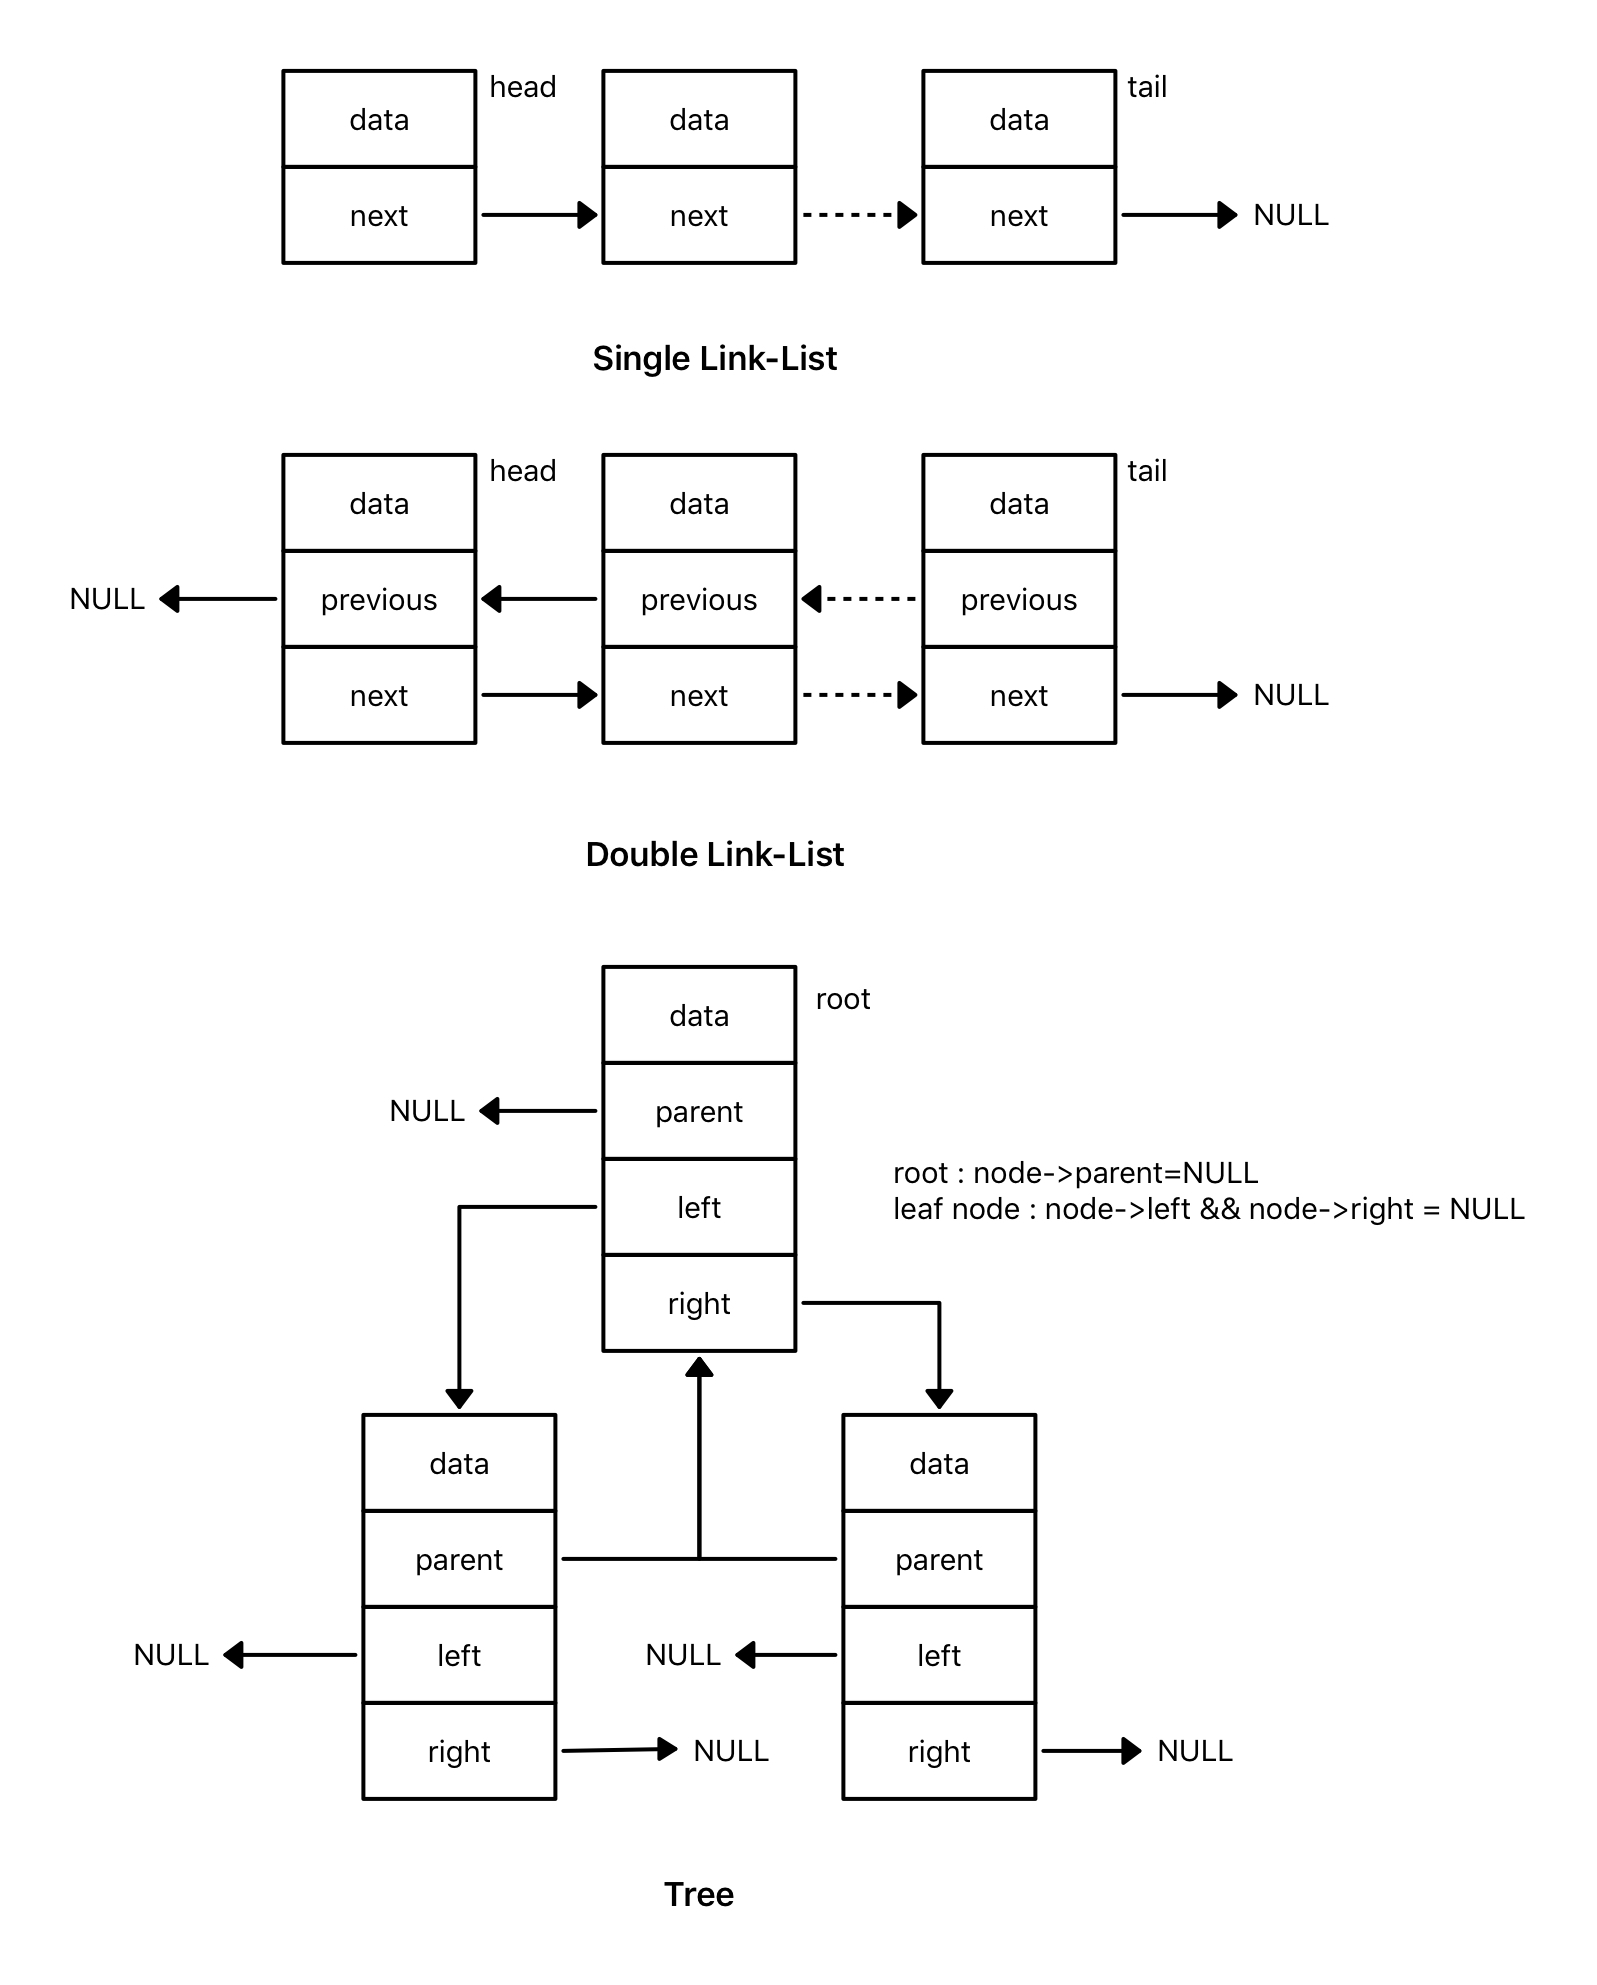
\includegraphics[width=0.8\textwidth]{newlists.jpg}}
\caption{Linked lists: (Top) Single LL (Middle) Double LL (Bottom) Tree}
\label{list}
\end{figure}

Figure \ref{list} show three types of data structure. The first is a single linked list that is unidirectional, next a double linked list that is bidirectional and finally a complete tree which is slightly more complex.

\subsubsection{Single linked lists}

A single linked list is a list structure where there is a single pointer pointing to the address of the next node in the list. The last node is identified as the node which points to NULL. Nodes can be inserted but all scans have to start from the beginning of the list.\\

\begin{lstlisting}[language=C,,showstringspaces=false,caption={File: llist1.c, single linked list},captionpos=b,label=linklist1]
 1 #include <stdio.h>
 2 #include <stdlib.h>
 3 #include <assert.h>
 4 
 5 typedef struct node
 6 {
 7 int data;
 8 struct node *next;
 9 } node_str;
10 
11 #define NEXT(s) s->next
12 #define DATA(s) s->data
13 
14 node_str *create_node(int value)
15 {
16 node_str *ptr;
17 
18 ptr = (node_str*)malloc(sizeof(node_str));
19 
20   if (ptr==NULL)
21   {
22   perror("failed to allocate memory");
23   exit(EXIT_FAILURE);
24   }
25 
26 DATA(ptr) = value;
27 NEXT(ptr) = NULL;
28 return ptr;
29 }
30 
31 void display(node_str *n)
32 {
33 assert(n!=NULL);
34 
35 printf("Single Linked list \n");
36   do
37   {
38   printf("... addr : 0x%8.8x\n",(unsigned int)n);
39   printf("... data : %d\n",DATA(n));
40   printf("... next : 0x%8.8x\n\n",(unsigned int)NEXT(n));
41   n = NEXT(n);
42   }
43   while (n!=NULL);
44 }
45 
46 int main(void)
47 {
48 node_str *root;
49 
50 root=create_node(1);
51 NEXT(root) = create_node(2);
52 NEXT(NEXT(root)) = create_node(3);
53 
54 display(root);
55 
56 free(NEXT(NEXT(root)));
57 free(NEXT(root));
58 free(root);
59 return 0;
60 }

INTERACTIONS

$ cc llist1.c
$ ./a.out
Single Linked list 
... addr : 0xc9c02610
... data : 1
... next : 0xc9c02620

... addr : 0xc9c02620
... data : 2
... next : 0xc9c02630

... addr : 0xc9c02630
... data : 3
... next : 0x00000000
$
\end{lstlisting}

Listing \ref{linklist1} shows the code that creates a single linked list of three nodes. Each node points to the next node in succession. As mentioned previously the last node points to NULL indicating that it is the last node in the list. 

Line:11:12 are useful macros that help with the linked list as it can get confusing when dealing with more complicated structures.

The first root node(1) is created and the data value set to 1. Then the pointer to next node(1) is assigned to the newly created node(2). This is repeated one more time until there is a linked list of three nodes created with each node pointing to the next.  

Finally we can see the output from the program and how the addresses relate to a single linked list. The root node is denoted by the data value 1 and the last node is denoted with data value 3.

\subsubsection{Double linked lists}

A double linked list is exactly as it sounds. In addition to a single link to the next node there is another link to the previous node. This gets around the problem of scanning from the beginning of the list each time a specific node needs to be found or modified. This is useful when there are many nodes and lots of editing occurs on those nodes. 

With single linked lists there is only one unique node which is the last node that points to NULL. By contrast a double linked list has two unique nodes. The first node which has its previous pointer pointing to NULL and the last node.

\begin{lstlisting}[language=C,caption={File: llist2.c, double linked list},showstringspaces=false,captionpos=b,label=linklist2]

 1 #include <stdio.h>
 2 #include <stdlib.h>
 3 #include <assert.h>
 4 
 5 typedef struct node
 6 {
 7 int data;
 8 struct node *previous;
 9 struct node *next;
10 } node_str;
11 
12 #define NEXT(s) s->next
13 #define LAST(s) s->previous
14 #define DATA(s) s->data
15 
16 node_str *create_node(int value)
17 {
18 node_str *ptr;
19 
20 ptr = (node_str*)malloc(sizeof(node_str));
21 
22   if (ptr==NULL)
23   {
24   perror("failed to allocate memory");
25   exit(EXIT_FAILURE);
26   }
27 
28 DATA(ptr) = value;
29 NEXT(ptr) = NULL;
30 LAST(ptr) = NULL;
31 return ptr;
32 }
33 
34 void display(node_str *n)
35 {
36 assert(n!=NULL);
37 
38 printf("Double Linked List \n");
39   do
40   {
41   printf("... addr : 0x%8.8x\n",(unsigned int)n);
42   printf("... data : %d\n",DATA(n));
43   printf("... prev : 0x%8.8x\n",(unsigned int)LAST(n));
44   printf("... next : 0x%8.8x\n\n",(unsigned int)NEXT(n));
45   n = NEXT(n);
46   }
47   while (n!=NULL);
48 }
49 
50 int main(void)
51 {
52 node_str *root;
53 
54 root=create_node(1);
55 NEXT(root) = create_node(2);
56 LAST(NEXT(root)) = root;
57 NEXT(NEXT(root)) = create_node(3);
58 LAST(NEXT(NEXT(root))) = NEXT(root);
59 display(root);
60 
61 free(NEXT(NEXT(root)));
62 free(NEXT(root));
63 free(root);
64 
65 return 0;
66 }

INTERACTIONS

$ cc llist2.c
$ ./a.out
Double Linked List 
... addr : 0x41c02610
... data : 1
... prev : 0x00000000
... next : 0x41c02630

... addr : 0x41c02630
... data : 2
... prev : 0x41c02610
... next : 0x41c02650

... addr : 0x41c02650
... data : 3
... prev : 0x41c02630
... next : 0x00000000
$

\end{lstlisting}

Listing \ref{linklist2} shows the code for a double linked list. It is similar to a single linked list but it includes an extra pointer to the previous node, as defined on line:8. Every time a node is added to the list both the previous link and the previous node's next link are updated. 

Double linked lists allow for a cursor-like concept, we can scan forwards as well as backwards within the list. To insert a new list into an existing list requires only 4 links to be updated. The links connected to the nodes around the insertion point in the original list. As well as the links in the head and tail of the new list require updating. This technique allows large insertions without major modifications to the original structure.  

\subsubsection{Tree}

A tree is a hierarchical structure where each node can have multiple child nodes, normally referred to as the left and right children in the case of a binary tree. A tree can be searched in multiple ways, for example depth-first or breadth-first. There are three traversal order available when search trees i.e. infix, postfix and prefix. This is best illustrated with an example. 

If we use a simple tree with 3 nodes, a parent node and two child nodes i.e. left and right. The parent is the + operator and the left child is x and the right child is y. A infix traversal order would be x + y, postfix traversal order is x y + and finally the prefix traversal is + x y. The traversal order is the order the nodes are visited. This is particularly useful when evaluating and dealing with expressions.

\begin{lstlisting}[language=C,showstringspaces=false,caption={File: llist3.c, binary tree structure},captionpos=b,label=linklist3]

 1 #include <stdio.h>
 2 #include <stdlib.h>
 3 #include <assert.h>
 4 
 5 typedef struct node
 6 {
 7 int data;
 8 struct node *parent;
 9 struct node *left;
10 struct node *right;
11 } node_str;
12 
13 #define LEFT(s)   s->left
14 #define RIGHT(s)  s->right
15 #define PARENT(s) s->parent
16 #define DATA(s)   s->data
17 #define LEFTSIDE  1
18 #define RIGHTSIDE 2
19 
20 node_str *create_node(int value)
21 {
22 node_str *ptr;
23 
24 ptr = (node_str*) malloc(sizeof(node_str));
25 
26   if (ptr==NULL)
27   {
28   perror ("failed to allocate memory");
29   exit (EXIT_FAILURE);
30   }
31 
32 DATA(ptr)   = value;
33 LEFT(ptr)   = NULL;
34 RIGHT(ptr)   = NULL;
35 PARENT(ptr) = NULL;
36 return ptr;
37 }
38 
39 void display (node_str *n)
40 {
41   if (n==NULL) return;
42 
43   printf ("... addr   : 0x%8.8x\n",(unsigned int)n);
44   printf ("... data   : %d\n",DATA(n));
45   printf ("... parent : 0x%8.8x\n",(unsigned int)PARENT(n));
46   printf ("... left   : 0x%8.8x\n",(unsigned int)LEFT(n));
47   printf ("... right  : 0x%8.8x\n\n",(unsigned int)RIGHT(n));
48   
49   display (LEFT(n));
50   display (RIGHT(n));
51 }
52 
53 void free_tree(node_str *n)
54 {
55   if (n==NULL) return;
56 
57 free_tree(LEFT(n));
58 free_tree(RIGHT(n));
59 
60 printf ("... free(ing) 0x%8.8x\n",(unsigned int)n);
61 free(n);
62 }
63 
64 node_str *attach(node_str *r,node_str *a, int mode)
65 {
66 assert ((mode==LEFTSIDE) ||  (mode==RIGHTSIDE));
67 assert (r!=NULL);
68 assert (a!=NULL);
69 
70   switch(mode)
71   {
72   case LEFTSIDE:
73   LEFT(r) = a;
74   break;
75 
76   case RIGHTSIDE:
77   RIGHT(r) = a;
78   break;
79   }
80 
81 PARENT(a) = r;
82 return a;
83 }
84 
85 int main (void)
86 {
87 node_str *root;
88 node_str *tmp;
89 
90 root=create_node (1);
91 tmp = attach (root,create_node(2),LEFTSIDE);
92 tmp = attach (root,create_node(3),RIGHTSIDE);
93 attach (tmp,create_node(4),LEFTSIDE);
94 
95 printf ("Binary Tree Linked list \n");
96 display (root);
97 free_tree(root);
98 
99 return 0;
100 }

INTERACTIONS

$ cc llist3.c
$ ./a.out
Binary Tree Linked list 
... addr   : 0xb5402610
... data   : 1
... parent : 0x00000000
... left   : 0xb5402630
... right  : 0xb5402650

... addr   : 0xb5402630
... data   : 2
... parent : 0xb5402610
... left   : 0x00000000
... right  : 0x00000000

... addr   : 0xb5402650
... data   : 3
... parent : 0xb5402610
... left   : 0xb5402670
... right  : 0x00000000

... addr   : 0xb5402670
... data   : 4
... parent : 0xb5402650
... left   : 0x00000000
... right  : 0x00000000

... free(ing) 0xb5402630
... free(ing) 0xb5402670
... free(ing) 0xb5402650
... free(ing) 0xb5402610
$
\end{lstlisting}

Listing \ref{linklist3} implements a tree with two children. Each node contains three pointers. A left and right link to each child and a parent link pointing to the parent node. 

A leaf node is identified as having no children, i.e. both left and right pointers are NULL (see nodes(2) and (4)). The root node(1) is the node where the parent link points to NULL. 

This program uses recursion for both \textit{display(...)} and \textit{free\_tree(...)} functions. Recursion is a Computer Science technique where a function calls itself. The \textit{display(...)} function uses a prefix top-down recursive algorithm whereas \textit{free\_tree(...)} function uses a postfix bottom-up recursive algorithm.

For deeply embedded or safety-critical systems, recursion is discouraged because recursion can require an unknown amount of stack space, also there is the possibility that the result becomes divergent (doesn't come to an end).

\newpage
\section{Input/Output} \label{IO}

Input/Output, or simply I/O, is a fundamental feature of all programming languages. The C language is no exception. I/O allows a program to communicate with the outside world. This communication is through the use of files and streams. File access is used to do everything from produce text files to accessing hardware peripherals. Also C provides three standard streams for input, output and errors.  

The underlying details of I/O tend to be dependent on the actual Operating System. By contrast the C language provides a generic set of functions to open streams and access files. Many of these mechanisms have already been introduced. For instance, \textit{fprintf(...)} to print out errors to the console.

\subsection{Standard streams}

The C Programming Language provides three standard streams to control input, output and errors. These streams are called \textit{stdin}, \textit{stdout} and \textit{stderr} respectively. 

\index{stdin}
\index{stdout}
\index{stderr}

\begin{description}
  \item[$\bullet$] \textbf{stdin}, standard input from a device e.g. keyboard 
  \item[$\bullet$] \textbf{stdout}, standard output sends to a device e.g. console  
  \item[$\bullet$] \textbf{stderr}, standard error send to a device e.g. error file or console
\end{description}

They can be redirected to point to different devices. These streams are always available and can buffered differently depending upon the requirement. Buffering can be set to one of three types, namely \textit{fully buffered}, \textit{line buffered} or \textit{unbuffered}. \textit{Fully buffered} only returns once the buffer is full. \textit{Line buffered} returns when a end-of-line occurs (i.e. return key is pressed) and \textit{unbuffered} is simply no buffer. These streams are used to interface with the outside world. 

For embedded systems, these streams are the first functionality you should get working when bringing up a new hardware platform. 

\subsubsection{stdin}

Normally defined as the hardware keyboard for a command line console. When a key is pressed on the keyboard the key value is placed into the stdin stream to be used by a program. The stdin can be thought to be a buffer so more than one key may be in the stdin stream ready to be read.

\begin{lstlisting}[language=C,showstringspaces=false,caption={File: getchar.c},captionpos=b,label=getchar]
	
 1 #include <stdio.h>
 2 
 3 int main(void)
 4 {
 5 char c;
 6 
 7 printf ("press any key and then return-key \n");
 8 
 9   do
10   {
11   c = getchar();
12   printf ("%d pressed \n",c);
13   }
14   while (c!='e');
15 
16 printf("... complete\n");
17 return 0;
18 }

INTERACTION

$ ./a.out
press any key and then return-key 
a
97 pressed 
10 pressed 
b
98 pressed 
10 pressed 
e
101 pressed 
... complete
$
 
\end{lstlisting}

Listing \ref{getchar} shows a program which loops around requesting a key to be pressed. Each time the key is pressed a return-key also has to be pressed for the buffer to be sent. This can be seen in the INTERACTION section, where a key pressed is followed by 10 pressed (10 represents the return key value). Also note that the character is echoed to the console not by the program but by the command line. 

Line:11 shows a function called \textit{getchar(...)}. This function is equivalent to \textit{getc(stdin)}, where \textit{stdin} is the standard input stream.

\subsubsection{stdout}

As mentioned at the beginning of this section, we have been using this stream extensively throughout this book. A good example of \textit{stdout} is the function \textit{printf(...)} used in the first program presented. \textit{printf(...)} sends characters to the \textit{stdout} stream. Normally this is set to the console but can also be redirected to a file or other hardware device. There are multiple functions can take advantage of \textit{stdout}, we will just focus on the \textit{printf(...)} function.

\index{printf(...)}

The \textit{printf(...)} function takes in a variable number of arguments. It uses a a concept called \textit{varargs} which allows multiple arguments without specifying a fixed number. This is useful as it allows different combinations of output formats. A subset of the formats available are outlined below.\newpage

\begin{table*}[ht]
\centering
  \begin{tabular}{ | l | l |}
    \hline
    FORMAT & TYPE \\ \hline
    \%x & Unsigned hexadecimal integer \\ \hline
    \%c & Character \\ \hline
    \%d & Signed decimal integer \\ \hline
    \%s & String of characters \\ \hline
    \%f & Decimal floating point \\ \hline
  \end{tabular}
\caption{Field formats}
\label{table:fformats}
\end{table*}

Table \ref{table:fformats} shows a common subset of the various formats. There are many other formats available. 

\begin{lstlisting}[language=C,showstringspaces=false,caption={File: fprintf.c},captionpos=b,label=myfprintf]

 1 #include <stdio.h>
 2 
 3 int main(void)
 4 {
 5 float f = 3.14159265;
 6 int i = 1223456;
 7 char s[] = "Hello";
 8 char c = 'a';
 9 
10 printf("%f,%d,0x%x,\"%s\",%c\n",f,i,i,s,c);
11 fprintf(stdout,"%f,%d,0x%x,%s,%c\n",f,i,i,s,c);
12 
13 return 0;
14 }  

INTERACTION

$ cc fprintf.c
$ ./a.out
3.141593,1223456,0x12ab20,"Hello",a
3.141593,1223456,0x12ab20,Hello,a
$ 

\end{lstlisting}

Listing \ref{myfprintf} shows that \textit{printf(...)} on line:10 and \textit{fprintf(...)} on line:11 are equivalent. \textit{printf(...)} streams everything to \textit{stdout}. Note that the format for hexadecimal using \textit{\%8.8x} directs the \textit{printf(...)} to present a 8 character hexadecimal number with leading 0's. This is useful when representing hardware registers.   

\subsubsection{stderr}

\index{stderr}

Again we have covered \textit{stderr} in more detail in section \ref{errors}, so rather than repeating an example we recommend going back and taking a look at that section. The buffer for this stream is set to \textit{unbuffered} as the output information will be required immediately.

\subsection{File I/O}

File I/O refer to the operations on files that reside on a filing system. These files can be a database, text, binary, etc.. They can be opened for writing, reading and updating. The files can be locked or unlocked for  sequential or random access. Again it should be noted that the underlying Operating System may have many more functions to control file I/O.
  
\subsubsection{Access control}

Access control is the mechanism to stop multiple programs accessing the same file at the same time. This is important since in a Unix like operating system many programs may want to access the same files and corruption could easily occur unless there are some safeguards.

\index{fopen(...)}
\index{fclose(...)}

For C, access control is achieved using two function calls, namely \textit{fopen(...)} and \textit{fclose(...)}. These functions lock and unlock files. The \textit{fopen(...)} function locks a file resource so no other program can gain access and \textit{fclose(...)} does the reverse, it releases a locked file resource so other programs can gain access.
 
\textit{fopen(...)} defines which file is locked and the type of file which will be locked i.e. read only, write only, read-write, create, append, etc.. If the function is successful a non-NULL FILE pointer is returned, otherwise NULL is returned. The FILE pointer points to a hidden file descriptor which is used by the other file functions. \textit{fopen(...)} opens a stream to a specific file and \textit{fclose(...)} closes the stream.
 
\begin{table}
\centering
  \begin{tabular}{ | l | l |}
    \hline
    MODE & ACTION \\ \hline
    r & open text file for reading \\ \hline
    rb & open binary file for reading \\ \hline
    r+ & open for reading and writing \\ \hline
    w & create text file for writing \\ \hline
    wb & create binary file for writing \\ \hline
    w+ & open a text file or create if nonexistent \\ \hline
    a & append, write at end of file \\ \hline
    a+ & reading and writing at end of file \\ \hline
  \end{tabular}
\caption{File attributes}
\label{fopenformat}
\end{table}

The table \ref{fopenformat} includes both binary and text file open options. A binary file contains non-readable characters. An example of a binary file is an object file produced by the compiler. Binary files should not be loaded into a text editor unless the editor has been specifically designed to handle this type of editing.

\begin{lstlisting}[language=C,showstringspaces=false,caption={File: fopen.c},captionpos=b,label=fopen]

 1 #include <stdio.h>
 2 #include <stdlib.h>
 3 #include <time.h>
 4 
 5 int main(void)
 6 {
 7 FILE *HANDLE;
 8 time_t seconds;
 9 
10 HANDLE = fopen("seconds.dat","w");
11 
12   if (HANDLE == NULL)
13   {
14   perror("seconds.dat");
15   exit(EXIT_FAILURE);
16   }
17 
18 seconds = time(NULL);
19 fprintf(HANDLE,"%ld",seconds);
20 fclose(HANDLE);
21 return 0;
22 }

INTERACTION

$ cc fopen.c
$ ./a.out
$ more seconds.dat
1502813680
$

\end{lstlisting}

Listing \ref{fopen} shows code that opens a text file for writing, gets the current Unix time in seconds and then writes the time out to a file. Unix time is the number of seconds since 00:00:00 Universal Time Coordinated (UTC), 1 January 1970. The file opened is \textit{seconds.dat} on line:10 and the file is opened with the \textit{w} options (write only). Notice that the same \textit{fprintf(...)} function is used to write out using the file \textit{HANDLE}. Finally the file is released on line:20 with a call to \textit{fclose(...)}

\subsubsection{fscanf(...)}

The \textit{fscanf(...)} function reads from a specific stream or file handle. The same format options can be used as with the \textit{printf(...)} function. Using the same formats makes it relatively easy to write and then read in information from a file.

\index{fscanf(...)}

\begin{lstlisting}[language=C,showstringspaces=false, caption={File: fscanf.c},captionpos=b,label=fscanf]

 1 #include <stdio.h>
 2 #include <stdlib.h>
 3 #include <time.h>
 4 
 5 int main(void)
 6 {
 7 FILE *HANDLE;
 8 time_t seconds;
 9 
10 HANDLE = fopen("seconds.dat","r");
11 
12   if (HANLDE == NULL)
13   {
14   perror("seconds.dat");
15   exit(EXIT_FAILURE);
16   }
17 
18 fscanf(HANDLE,"%ld",&seconds);
19 printf("record Unix time is: %ld\n",seconds);
20 fclose(HANDLE);
21 return 0;
22 }

INTERACTION

$ cc fscanf.c
$ ./a.out
record Unix time is: 1502813680
$ 

\end{lstlisting}

Listing \ref{fscanf} shows code that opens a read-only file. Line:10 opens the file called \textit{seconds.dat}. Data is then extracted from the file on line:18. The extracted data is of type \textit{signed long int} and is specified using \textit{\%ld} directive. The data value is then placed into the variable \textit{seconds}. \textit{seconds} is specified as being of type \textit{time\_t} (or \textit{signed long int}). Note the variable is accessed by reference, meaning the data is placed at the address of the variable. The INTERACTION part shows the number of seconds being read and displayed on the console command line. This is the same number that was written to the file in listing \ref{fopen}.


\subsection{Parsing using file I/O}

Lets take a look at a more complicated example. We take an existing solution that used strings and convert it to using file i/o. This conversion makes the solution more general and flexible, replacing hardcoded fixed strings with data files.

\index{fgetc(...)}

\begin{lstlisting}[language=C,showstringspaces=false, caption={File: fgetc.c},captionpos=b,label=fgetc]

 1 #include <stdio.h>
 2 #include <stdlib.h>
 3 #include <stdint.h>
 4 
 5 /* macros */
 6 #define NO_TRANSITION -1
 7 
 8 /* new datatypes */
 9 typedef struct
10 {
11 char c;
12 uint8_t state;
13 uint8_t new_state;
14 int (*function) (int);
15 } states_str;
16 
17 /* function prototypes */
18 int ident(int loc);
19 int record(int loc);
20 
21 /* globals */
22 
23 int at=-1;
24 
25 states_str states[] =
26 {
27 'h',	0,	1,	record,
28 'h',	1,	1,	record,
29 'e',	1,	2,	NULL,
30 'l',	2,	3,	NULL,
31 'l',	3,	4,	NULL,
32 'o',	4,	0,	ident,
33  0 ,	0,	0,	NULL
34 };
35 
36 /* functions */
37 int record(int loc)
38 {
39 at = loc;
40 return 0;
41 }
42 
43 int ident(int loc)
44 {
45 printf("... search string 'hello' found at %d\n",at);
46 return 1;
47 }
48 
49 int state_machine(char *title,char *filename)
50 {
51 FILE *handle;
52 int scan;
53 int current=0; // start state
54 int transition;
55 int num;
56 char c;
57 
58 printf("%s: \"%s\"\n",title,filename);
59 num = 0;
60 
61 handle = fopen(filename,"r");
62  
63    if (handle == NULL)
64    {
65    fprintf (stderr,"error: couldn't open %s\n",filename);
66    exit(EXIT_FAILURE);
67    }
68 
69 c = fgetc(handle);
70 
71   while (c != EOF)
72   {
73   scan = 0; // reset scan
74   transition = NO_TRANSITION; 
75 
76     while (states[scan].c !=0 )
77     {
78       if (c == states[scan].c && current == states[scan].state)
79         transition = scan;
80     scan++;
81     }
82 
83     if (transition == NO_TRANSITION)
84       current = 0; // reset state
85     else
86     {
87     current = states[transition].new_state;
88       if (states[transition].function!=NULL)
89         num += states[transition].function((int)(ftell(handle)-1));  
90     }
91   c = fgetc(handle);
92   }
93 
94 printf("... strings: %d\n",num);
95 fclose(handle);
96 return num;
97 } 
98 
99 int main(void)
100 {
101 state_machine("test 1","string1.dat");
102 state_machine("test 2","string2.dat");
103 state_machine("test 3","string3.dat");
104 state_machine("test 4","string4.dat");
105 state_machine("test 5","string5.dat");
106 state_machine("test 6","string6.dat");
107 return 0;
108 }

INTERACTION

$ cc fgetc.c
$ ./a.out
test 1: "string1.dat"
... search string 'hello' found at 13
... strings: 1
test 2: "string2.dat"
... strings: 0
test 3: "string3.dat"
... strings: 0
test 4: "string4.dat"
... search string 'hello' found at 11
... search string 'hello' found at 28
... strings: 2
test 5: "string5.dat"
... search string 'hello' found at 25
... strings: 1
test 6: "string6.dat"
... search string 'hello' found at 7
... search string 'hello' found at 12
... search string 'hello' found at 17
... strings: 3
$

\end{lstlisting}

Listing \ref{fgetc} shows the same parsing program used in listing \ref{table} on page \pageref{tablee} with a few exceptions. Line:61 uses \textit{fopen(...)} to open a text file. Line:69 uses \textit{fgetc(...)} to input a character at a time. Line:71 checks that the end-of-file (EOF) hasn't been reached. Line:89 records the location in the file using the function \textit{ftell(...)}. Finally line:95 closes the file with \textit{fclose(...)}. If we compare the INTERACTION parts, we find that it is identical to the fixed string code. The only real difference is that the data source is a file. 

\index{fgetc(...)}
\index{ftell(...)}
 
  
\newpage
\section{Time} \label{Time}

Time can be described in two quantities, namely the actual time and the measurement of time. Both critically important for embedded and real-time systems. Time is used for many tasks, from setting up a future event to measuring the number of cycles between two relative points. To be clear each hardware platform can provide much better precision or accuracy than what is provided by the standard \textit{time.h} library. The main role of the time library is to provide some consistent precision and accuracy between platforms.  

\textit{Actual time} is the time displayed on a clock or calendar e.g. hh:mm 12:45 PM, hh:mm:ss 1:45:23 AM, yyyy/mm/dd 2018/01/28. By comparison, \textit{measurement-of-time} can be calculated between actual time points (i.e. seconds, minutes, ..., day, years, etc.) or by clock ticks. Clock ticks are \textit{virtual} ticks that have been normalized to 1,000,000 \textit{ticks-per-second}. Depending upon the requirement clock ticks can be of less value. 

\subsection{clock\_t, time\_t and struct tm}

The \textit{time.h} library provides a set of useful functions to access time and date. These functions rely on three important data structures, namely \textit{clock\_t}, \textit{time\_t} and finally \textit{struct tm}. The data structures are used to store and manipulate different forms of time as described below.

\begin{itemize}
  \item[$\bullet$] \textbf{clock\_t}: is a measurement of clock ticks. It is an arithmetic measurement with \textit{CLOCKS\_PER\_SEC} being a constant representing the number of clock ticks per second. It is used in conjunction with the \textit{clock(...)} function to measure processor time. This is amount of time used by the processor. See section \ref{clockss} for more details and a working example.
  \item[$\bullet$] \textbf{time\_t}: is referred to as calendar time. Even-though not specified by the C standard, it is commonly identified as the number of seconds since 00:00, Jan 1 1970 UTC. This is also known as POSIX time. Prior to the release of the C11 standard it was arithmetic and post C11 it became a real number. See section \ref{timet} for more details. 
  \item[$\bullet$] \textbf{struct tm}: this data structure holds the time and date data
\end{itemize}

\index{clock\_t} \index{time\_t} \index{struct tm}

\subsection{clock(...)} \label{clockss} \index{clock(...)}

The \textit{clock(...)} function returns the number of clock ticks (type \textit{clock\_t}). It can be used to calculate the number of seconds by dividing the clock ticks by the constant  \textit{CLOCKS\_PER\_SECOND}. See listing \ref{clock} below.
 
\begin{lstlisting}[language=C,showstringspaces=false,caption={File: clock.c},captionpos=b,label=clock]

 1 #include <stdio.h>
 2 #include <unistd.h>
 3 #include <time.h>
 4 #include <stdint.h>
 5 
 6 int main(void)
 7 {
 8 clock_t start,end;
 9 double proc_time;
10 uint32_t i;
11 
12 printf ("...... start loop\n");
13 start = clock();
14 i = 100000000;
15   while(--i) ;
16 end = clock();
17 
18 proc_time = (end-start) / (double) CLOCKS_PER_SEC;
19 
20 printf("...... start time: %ld\n",start);
21 printf("........ end time: %ld\n",end);
22 printf(".. CLOCKS_PER_SEC: %d\n",CLOCKS_PER_SEC);
23 printf(".. Processor time: %f seconds \n",proc_time);
24 
25 return 0;
26 }

INTERACTION

* Desktop PC

27 $ cc clock.c
28 $ ./a.out
29 ...... start loop
30 ...... start time: 2855
31 ........ end time: 234425
32 .. CLOCKS_PER_SEC: 1000000
33 .. Processor time: 0.231570 seconds

* Embedded Device 

34 $ cc clock.c
35 $ ./a.out
36 ...... start loop
37 ...... start time: 3739
38 ........ end time: 610643
39 .. CLOCKS_PER_SEC: 1000000
40 .. Processor time: 0.606904 seconds 

\end{lstlisting}

The listing \ref{clock} shows two execution-runs. The first is on a UNIX Desktop and the second on a low-cost Embedded Device running Linux. The first execution-run line:33 is significantly faster than the second line:40. Even-though dissimilar devices both follow the same C APIs. Note that the \textit{CLOCKS\_PER\_SECOND} is the same number between both execution-runs because the clocks ticks are normalized.   

\subsection{time(...)} \label{timet} \index{time(...)}

The \textit{time(...)} function returns the number of seconds (type \textit{time\_t}). This is the number of seconds from the UNIX Epoch, or more precisely the number of seconds since 00:00, Jan 1 1970 UTC.   

\begin{lstlisting}[language=C,showstringspaces=false,caption={File: time.c},captionpos=b,label=ctime]

 1 #include <stdio.h>
 2 #include <unistd.h>
 3 #include <time.h>
 4
 5 int main(void)
 6 {
 7 time_t start,end;
 8 double time_taken;
 9 
10 time(&start);
11 sleep(5);
12 time(&end);
13
14 printf("......... start time: %ld\n",start);
15 printf("........... end time: %ld\n",end);
16 printf(".. second time taken: %f\n",difftime(end,start));
17
18 return 0;
19 }

INTERACTION

* Desktop PC

20 $ cc time.c
21 $ ./a.out
22 ......... start time: 1516720389
23 ........... end time: 1516720394
24 ......... time taken: 5.000000
25 $

* Embedded Device 

26 $ cc time.c
27 $ ./a.out
28 ......... start time: 1522522820
29 ........... end time: 1522522825
30 ......... time taken: 5.000000
31 $ 

\end{lstlisting}

The listing \ref{ctime} shows two execution-runs (similar to section \ref{clockss}). The difference is that the measured time is exactly the same 5 seconds (line:24 and line:30). The difference is time is calculated with a call to the \textit{difftime(...)} function on line:16.

\newpage
\subsection{struct tm} \index{struct tm}

The \textit{struct tm} is used when dealing with calendar dates and/or wall clock time. It is useful when a date and time marker is required. The structure members are defined in listing \ref{structtm} below.  

\begin{lstlisting}[language=C,showstringspaces=false,caption={Structure members: struct tm},captionpos=b,label=structtm]

int    tm_sec;   // seconds [0,61]
int    tm_min;   // minutes [0,59]
int    tm_hour;  // hour [0,23]
int    tm_mday;  // day of the month [1,31]
int    tm_mon;   // month of the year [0,11]
int    tm_year;  // years since 1900
int    tm_wday;  // day of the week [0,6] (Sunday = 0)
int    tm_yday;  // day of the year [0,365]
int    tm_isdst; // daylight savings flag

\end{lstlisting}

As can be seen the structure covers seconds, minutes, hours, day-of-the-month, month, year, weekday, day-of-the-year and finally daylight saving. Below listing \ref{ctm} is an example of how to use the structure in a programming context. 

\begin{lstlisting}[language=C,showstringspaces=false,caption={File: tm.c},captionpos=b,label=ctm]

 1 #include <stdio.h>
 2 #include <time.h>
 3
 4 int main(void)
 5 {
 6 time_t now;
 7 struct tm *time_info;
 8 char time_buffer[60];
 9
10 time(&now);
11 time_info = localtime(&now);
12
13 strftime(time_buffer,80,"%y/%m/%d %X",time_info);
14
15 printf("%s\n",time_buffer);
16 
17 return 0;
18 }

INTERACTION

19 $ cc tm.c
20 $ ./a.out
21 18/01/22 21:21:59
22 $

\end{lstlisting}

The C program simply writes out the year/month/day-of-the-month hour24:minutes:seconds, as shown on line:21. The \textit{locale} of the device is also important when it comes to time since it determines the timezone shifts for wall clock time. All the the timezone shifts occur from UTC time.











\newpage
\section{Miscellaneous}

This section contains some useful functions that don't fit into the framework but are really useful functions when programming. 

\subsection{system(...)}

\index{system(...)}

The \textit{system(...)} function is found in \textit{stdio.h}. It allows for interaction with the command line shell. This is useful when having to execute certain commands while under program control. Most of the commands available in Linux also have a program interface but sometimes it is easier to call the command directly via the host shell.\\

\begin{lstlisting}[language=C,showstringspaces=false, caption={File: system.c},captionpos=b,label=system]

 1 #include <stdio.h>
 2 #include <stdlib.h>
 3 
 4 int main(void)
 5 {
 6 FILE *HANDLE;
 7 char user[20];
 8 
 9   if (!system("whoami > me.dat"))
10     printf("success\n");
11   else
12     printf("failed\n");
13 
14 HANDLE=fopen("me.dat","r");
15 
16   if (HANDLE==NULL)
17   {
18   perror("file me.dat");
19   exit(EXIT_FAILURE);
20   }
21 
22 fscanf(HANDLE,"%s",user);
23 fclose(HANDLE);
24 
25 printf("user: %s\n",user);
26 
27 return 0;
28 }

INTERACTION

$ cc system.c
$ ./a.out
success
user: proteus
$

\end{lstlisting}

Listing \ref{system} shows code for a program which sends a command string to the shell. The command string both invokes the command \textit{whoami} and redirects the output to a file called \textit{me.dat} line:9. This file is then read and the active user name is then displayed on line:25. The INTERACTION part shows that the \textit{system(...)} function was successful and that the user is \textit{proteus}.

\subsection{sprintf(...)}

\index{sprintf(...)}

\textit{sprintf(...)} is a variation of the \textit{printf(...)} function. Instead of directing the output to a stream, it directs the output to a string. This can be extremely useful for a number of activities including building dynamic strings like file paths. Care has to be given that there is enough space for the created string.

\begin{lstlisting}[language=C,showstringspaces=false, caption={File: sprintf.c},captionpos=b,label=sprintf]

 1 #include <stdio.h>
 2 
 3 void new_file_path(char *filepath, char *filename)
 4 {
 5 sprintf(filepath,"project/special/%s",filename);
 6 }
 7 
 8 void clear(void)
 9 {    
10   while (getchar() != '\n' ); // clear stdin
11 }
12 
13 int main(void)
14 {
15 char project[40];
16 char filepath[256];
17 
18 printf("enter project  name?\n");
19 scanf("%s", project); // scan for user input
20 clear(); // clear buffer
21 new_file_path(filepath,project);
22 printf("filepath: %s\n",filepath);
23 
24 return 0;
25 }

INTERACTION

$ cc sprintf.c
$ ./a.out
enter project  name?
hello.c
filepath: project/special/hello.c
$

\end{lstlisting}

Listing \ref{sprintf} shows a program that takes user input, as shown on line:19. The input string \textit{project} is used to construct a file path string, shown on line:5. The program then outputs the newly created file path on line:22. In the INTERACTION part we can see that the user typed in \textit{hello.c}. The program then appended \textit{project/special/} onto the file name to give a complete file path of \textit{project/special/hello.c}.



  
\newpage
\section{Hints \& Tips}

The Hints \& Tips section focuses on Embedded, Real-Time and Safety-Critical recommendations. Below are a collection of useful experiences based on some of the standard guidelines (e.g. MISRA-C) recommended by organizations such as AUTOSAR and JPL (Jet Propulsion Laboratory). 

\subsection{General}

\begin{enumerate}

\item \textbf{Use assert(...)}: use wherever possible within a program, especially when developing source code. Even-through the code may be correct the data may not be correct. See section \ref{assert} on page \pageref{assert}.

\item \textbf{No recursion}: specifically for embedded systems, recursion should be avoided for two reasons. First the required stack size is unknown and second a recursive function is not guaranteed to converge. If non-convergence occurs either an exception is finally raised or data corruption occurs i.e. stack overflow. Recursion is a good technique especially when combined by proof-by-induction but it is not recommended for embedded or safety-critical systems.

\item \textbf{Dynamic memory}: should be avoided during runtime, since errors and corruption can occur that are difficult to handle in an embedded system. Dynamic memory can be used in controlled parts of the device lifecycle i.e. initialization and exit phase. Instead it is recommended that statically allocated memory is used or a directly managed fixed memory buffer.

\item \textbf{Functions}: keep simple and short. This makes functions easier to debug, optimize and test. 

\item \textbf{Commenting}: make sure each function is adequately commented, explaining purpose, input parameters, output and side-effects. 

\item \textbf{Run time error checking}: check for errors and determine a course of action when an error occurs. Course of action can be more complicated in an embedded or safety-critical system since simply stopping may not be a viable option.

\item \textbf{Warnings}: make sure that all warnings are removed from at compilation stage. This is important since warnings are indications that something is not quite right with the code. 

\item \textbf{Memory usage}: make sure that memory usage is carefully monitored during software development. Memory corruption is one of the factors that causes instability. This is especially important for embedded devices with limited memory.

\item \textbf{Control structures}: reduce the depth of deep nested control structures (e.g. \textit{if ... else }). Deep control structures are difficult to test and adds complexity to the source code. Complexity leads to instability.

\item \textbf{Equivalence ordering}: where possible when comparing a constant put the constant first. This allows the compiler to flag a wrong expression. For instance, "if (CONST\_VALUE==variable\_name)" is syntactically correct but "if (CONST\_VALUE=variable\_name)" produces a syntax error. Whereas both "if (variable\_name==CONST\_VALUE)" and "if (variable\_name=CONST\_VALUE)" are syntactically correct but result in completely different outcomes. This can result in an error which is difficult to discover. 

\item \textbf{Include time information in log output}: when designing logfile format it is always useful to consider including time information. This is important since time can be a major factor in identifying a real-time or embedded issue.

\item \textbf{Logging}: use \textit{printf(...)} or \textit{fprintf(...)} extensively throughout the code. It is a powerful tool for debugging and provides historical record on how a program is operating. \textit{printf(...)} function is a complicated function and takes up valuable compute cycles. This is important when dealing with Real-Time designs. There are special embedded versions for resource constrained devices.

\item \textbf{Don't optimize too early}: when developing C code don't attempt to optimize too quickly. It is quite easy to optimize code that doesn't significantly effect the overall performance of the system. Optimization frequently makes debugging more complicated.

\item \textbf{Style}: when working with existing code, try to keep to the style of that code. In other words don't attempt in introduce a new style unless the goal is to rewrite all the source to that new style.

\end{enumerate}

\subsection{Debugging}

\begin{enumerate}

\item \textbf{Possibilities:} create a list of possible-causes from likely to unlikely. This list tends to be dynamic and is constantly revisited. Depending on the complexity, the task of creating a list may be visited numerous times throughout the debug process.

\item \textbf{Experiment:} there is only so much you can gain from looking at code, it is important to start experimenting and modifying source. This helps with gaining a better understanding of the problem. Debugging is not a theoretical activity, experiment and gathering information.

\item \textbf{Divide and conquer:} try and break the problem into smaller manageable chunks, this involves pruning the problem space in to understandable elements i.e. follow the systematic \textit{scientific method} as much as possible.

\item \textbf{Avoid mysticism:} when the problem is hard there is a tendency to branch away from logic, this should be avoided. There are times when strangenesses do occur but these are rare and seldom events. More mythical ideas should be kept at the bottom of any possible-cause list.

\item \textbf{Explore the problem-domain:} be comfortable with letting go of any hypothesis but remember to keep each one as a possibility. Nothing is closed until there is a final resolution. There may be multiple causes to any one problem.

\item \textbf{Frameworks:} create an environment to gain more information. This may include extra hardware or setting up a simulation environment. Put effort into the discovery framework and gather data. 

\item \textbf{Think through the problem:} as the pieces come together go through the evidence carefully and try to explain what is the \textit{cause and effect}. Just verbally explaining and white-boarding a problem can help provide new motivations for exploration.

\item \textbf{Double-check:} capture all known errors, use \textit{assert(...)} extensively throughout the code. Make sure all compiler warnings are understood and removed. Make sure there is error coverage for both data and code.

\item \textbf{Keep debug code:} retain all debug code in the source. This is useful when other problems are being explored. The rule is that debug data is always important.

\item \textbf{Have fun:} enjoy debugging, James Joyce wrote \textit{"Mistakes are the portal of discovery"}. Debugging can be a really interesting and challenging activity. Why software fails is a science.

\end{enumerate}

  
\newpage
\section{Sources}

\subsection{Books}

Barr, Michael (1999) Programming Embedded Systems in C and C++, O'Reilly Media

Harbison, Samuel P. (2002) C: A Reference Manual, 5th Edition, Pearson

Kernighan, Brian W. (1988) C Programming Language, 2nd Edition Prentice Hall 

Klemens, Ben (2014) 21st Century C: C Tips from the New School 2nd Edition, O'Reilly Media

Plauger, P.J. (1992) The Standard C Library 1st Edition, Prentice Hall

Stevens, W. Richards (2013) Advanced Programming in the UNIX Environment, 3rd Edition 3rd Edition, Addison-Wesley Professional

\subsection{Online}

Assertion (software development) (n.d.). In Wikipedia, Retrieved August 21, 2017, \\from https://en.wikipedia.org/wiki/Assertion\_(software\_development)

C dynamic memory allocation (n.d.). In Wikipedia, Retrieved August 22, 2017, \\from https://en.wikipedia.org/wiki/C\_dynamic\_memory\_allocation

C standard library (n.d.). In Wikipedia, Retrieved August 21, 2017, \\from https://en.wikipedia.org/wiki/C\_standard\_library

C preprocessor (n.d.). In Wikipedia, Retrieved August 23rd, 2017, \\from https://en.wikipedia.org/wiki/C\_preprocessor

Memory Pool (n.d.). In Wikipedia, Retrieved August 26th, 2017, \\from https://en.wikipedia.org/wiki/Memory\_pool

Order of operations (n.d). In Wikipedia, Retrieved August 26th, 2017, \\from https://en.wikipedia.org/wiki/Order\_of\_operations

Memory barrier (n.d). In Wikipedia, Retrieved July 4th, 2018, \\from https://en.wikipedia.org/wiki/Memory\_barrier

Backus-Naur Form (n.d). In Wikipedia, Retrieved July 4th, 2018, \\https://en.wikipedia.org/wiki/Backus–Naur\_form

\subsection{Research}

Energy Efficiency across Programming Languages How Do Energy, Time, and Memory Relate?, Rui Pereira, Jacome Cunha, Marco Couto, Joao Paulo Fernandes, Francisco Ribeiro, Rui Rua, Joao Saraiva, Presented at SLE'17 October 2017.
  
\newpage
\printindex
\end{document}

